\documentclass[runningheads]{llncs}

%KYR: need to ensure included packages don't interfere with LNCS style
%\usepackage[utf8]{inputenc}
%\usepackage{amsthm, amsmath, amssymb}
\usepackage{amsfonts} %mathbb
\usepackage{amsmath} %hdots
\usepackage{amssymb} %blacksquare
\usepackage{mathabx} %vDash
\usepackage{mathrsfs} %mathscr
\usepackage{blkarray} %for blockarray
%\usepackage{textcomp}
%\usepackage{xcolor}
%\usepackage{soul}
%\usepackage{ dsfont }
\usepackage{hyperref}
\usepackage{cancel} %for \cancel
\usepackage{algorithm} %for algorithm environment
\usepackage{algcompatible}
\usepackage[noend]{algpseudocode}
%\usepackage{changepage}%http://ctan.org/pkg/changepage
\usepackage{graphicx} %for includegraphics
\usepackage{tikz}
\usepackage{lscape} %for landscape orientation
%\usepackage{float} %for figures
\usetikzlibrary{shapes.misc, positioning}
\usetikzlibrary{arrows.meta}
\tikzset{>={Latex[width=2mm,length=2mm]}}
\usepackage{caption}
\usepackage{mwe}
%% \hypersetup{
%%     colorlinks=true,
%%     linkcolor=blue,
%%     filecolor=magenta,
%%     urlcolor=red,
%%     citecolor=teal
%% }

%LNCS:
% If you use the hyperref package, please uncomment the following line
% to display URLs in blue roman font according to Springer's eBook style:
\renewcommand\UrlFont{\color{blue}\rmfamily}

%for qed:
%% \makeatletter
%% \newcommand{\pushright}[1]{\ifmeasuring@#1\else\omit\hfill$\displaystyle#1$\fi\ignorespaces}
%% \newcommand{\pushleft}[1]{\ifmeasuring@#1\else\omit$\displaystyle#1$\hfill\fi\ignorespaces}
%% \makeatother
%% \makeatletter
%% \newcommand{\specialcell}[1]{\ifmeasuring@#1\else\omit$\displaystyle#1$\ignorespaces\fi}
%% \makeatother


%%%%%%%%%%%%%%%%%%%%%%%%%%%%%%%%%%%%%%%%%%%%%%%%%%%%%%%%
% Spacing Magic
%%%%%%%%%%%%%%%%%%%%%%%%%%%%%%%%%%%%%%%%%%%%%%%%%%%%%%%%
%\usepackage{pslatex} % DON'T REMOVE!  BUYS US HALF A PAGE OR MORE!!!!!
%Use only in case of emergencies: \linespread{0.98} %KYR: make lines spaces .99 instead of 1 to save space
\usepackage{times} %KYR: substitute for pslatex that does not mess up math :)
%\usepackage{savetrees} %KYR: maybe also helps... if we can fix the text to enable this

\usepackage{enumitem}
\setlist[itemize]{noitemsep, nolistsep, topsep=0pt, partopsep={0pt}} 

%CAUTION: dirty trick; questionably allowed... use ONLY in case of emergencies!
% \linespread{0.99}

%%%%%%%%%%%%%%%%%%%%%%%%%%%%%%%%%%%%%%%%%%%%%%%%%%%%%%%%
% Figure Magic
%%%%%%%%%%%%%%%%%%%%%%%%%%%%%%%%%%%%%%%%%%%%%%%%%%%%%%%%
%\usepackage{epsfig}
\usepackage{float} % put figure in minipage
%\usepackage{framed}
%\usepackage{subfigure}

% diagonal line in the table
%\usepackage{diagbox}

\usepackage{enumitem}
\newlist{Properties}{enumerate}{2}
\setlist[Properties]{label=Property \arabic*.,itemindent=*}

%\usepackage{tikz}
%\newcommand*\circled[1]{\tikz[baseline=(char.base)]{
%            \node[shape=circle,draw,inner sep=0.5pt] (char) {#1};}}
%
%\newcommand{\VarPhiSequence}{\ensuremath{\langle T_{\varphi} \rangle}\xspace}
%\newcommand{\ExSeq}[1]{\ensuremath{\langle T_{#1} \rangle}\xspace}
%\newcommand{\ExSeqElement}[2]{\ensuremath{\langle T^{#1}_{#2} \rangle}\xspace}
%\newcommand{\IN}{\mathbb{N}}  

% draw box around text
\usepackage{tcolorbox} 

\renewcommand{\topfraction}{.99} %figures can take up at most 99% of the page before being alone
\renewcommand{\bottomfraction}{.99} %figures can take up at most 99% of the page before being alone
\renewcommand{\textfraction}{.01} %at most this % of page will be text before making figure-only page
\addtolength{\textfloatsep}{-5mm}
\addtolength{\floatsep}{-5mm}
\addtolength{\intextsep}{-5mm}
\addtolength{\abovecaptionskip}{-3mm}
\addtolength{\belowcaptionskip}{-2mm}

%%%%%%%%%%%%%%%%%%%%%%%%%%%%%%%%%%%%%%%%%%%%%%%%%%%%%%%%


\renewcommand{\phi}{\varphi}

%\theoremstyle{definition}
%\newtheorem{proposition}{Proposition}
%\newtheorem{remark}{Remark}
%\newtheorem{example}{Example}
%\newtheorem{definition}{Definition}
%\newtheorem{theorem}{Theorem}
%\newtheorem{lemma}{Lemma}

\newcommand{\R}{\mathbb{R}}
\newcommand{\C}{\mathbb{C}}
\newcommand{\Z}{\mathbb{Z}}

\def\nuXmv{{\sf nuXmv}\xspace}

\begin{document}
%
%\title{Contribution Title\thanks{Supported by organization x.}}
\title{Mission-time LTL (MLTL) Formula Validation Via Regular Expressions\thanks{Work supported in part by [omitted for blind review] {\bf Note that all references to appendices will be replaced with URLs in the final paper; they are appendices only for blind review.}}}
%
\titlerunning{Abbreviated paper title}
% If the paper title is too long for the running head, you can set
% an abbreviated paper title here
%
%\author{First Author\inst{1}\orcidID{0000-1111-2222-3333} \and
%Second Author\inst{2,3}\orcidID{1111-2222-3333-4444} \and
%Third Author\inst{3}\orcidID{2222--3333-4444-5555}}
%\author{Jenna Elwing\thanks{University of Michigan, Ann Arbor} \and Laura Gamboa Guzmán\thanks{Iowa State University} \and Jeremy Sorkin\thanks{The Ohio State University} \and Chiara Travesset\thanks{Purdue University} \and Zili Wang\thanks{University of California, Berkeley} \and Kristin Y. Rozier\footnotemark[2]}
%
%\authorrunning{F. Author et al.}
% First names are abbreviated in the running head.
% If there are more than two authors, 'et al.' is used.
%
%\institute{Princeton University, Princeton NJ 08544, USA \and
%Springer Heidelberg, Tiergartenstr. 17, 69121 Heidelberg, Germany
%\email{lncs@springer.com}\\
%\url{http://www.springer.com/gp/computer-science/lncs} \and
%ABC Institute, Rupert-Karls-University Heidelberg, Heidelberg, Germany\\
%\email{\{abc,lncs\}@uni-heidelberg.de}}
%
\maketitle              % typeset the header of the contribution
%




\vspace{-0.1in}
\begin{abstract}
        \noindent Mission-time Linear Temporal Logic (MLTL) is an extension of propositional logic that allows temporal quantifiers over finite discrete intervals. A computation is a finite sequence of truth assignments. In this paper, we use regular expressions to describe the structure of the computations that satisfy a given MLTL formula. We prove soundness and completeness of our structure. We also give an implemented algorithm (the WEST program) and analyze its complexity both theoretically and experimentally. Finally, we generate a test suite using control flow diagrams to robustly test the code.

        %We demonstrate that formula validation examples generated via regular expressions encapsulating the sets of all satisfying/unsatisfying assingments is tractable, both theoreteically and experimentally. We present an efficient algorithm for automatic characterization of an MLTL formula by its satisfying assingments, proove the theoretical correctness, time complexisty, and space complexity of hte algorithm. Then we provide a robust implementattion of the algorithm, demonstrate expreimentally its performance and correctness, and utilize intelligent fuzzing to increaes confidence int eh resulting open-source tool, which we release for public use. The result of our contributions are improvements to existing algorithms for MLTL analsysis applicable to many other tools and a new tool called WEST for provably correct, atomated, efficient MLTL formula validation.%
%        Our work connects existing tools to enable improvmeents in satisfiabiity tools and automated synthesis of verified code from MLTL behavior descriptions.

        \vspace{-0.1in}
\keywords{First keyword  \and Second keyword \and Another keyword.}
\end{abstract}

\vspace{-0.1in}
\section{Introduction}
\vspace{-0.1in}
System specifications, such as aerospace operational concepts, often utilize timelines to express critical requirements. We can cite examples of this from NASA's Automated Airspace Concept \cite{EH10}, the U.~S.~Navy's Aircraft Carrier Deck Scheduler \cite{RCRBS11}, the JAXA-NASA Global Precipitation Measurement (GPM) Observatory \cite{GPM}, and many others. Formal methods provide continuously-advancing tools and techniques to rigorously analyze timelines expressed in the form of temporal logic requirements, from early design-time model checking and theorem proving to on-board runtime verification. The U.~S.~Federal Aviation Administration (FAA) even advocates the use of formal methods for flight certification of these critical systems \cite{DO-178C,DO-254,DO-333}. Yet, a significant hurdle to the use of formal methods remains: how to convincingly demonstrate to the humans in the loop, from system designers to certifiers, that the analyzed formulas truly represent the system requirements \cite{Roz16}. We creatively address this validation question using regular expressions and truth tables.

NASA, for example, has developed several tools that operate over temporal logic requirements, such as FRET\cite{GMRPSS20}, R2U2\cite{RS17}, and a PVS library \cite{CTGPD22} for the logic MLTL (Mission-time Linear Temporal Logic) \cite{RRS14,LVR22}. MLTL was the logic used recently in NASA's Robonaut2 verification project \cite{KZJZR20} and is being used currently for both design-time and runtime verification of the NASA Lunar Gateway Vehicle System Manager \cite{DBR21}. Other recent verification %verification-for-certification
efforts involving MLTL include a JAXA autonomous satellite \cite{JAXA}, a UAS Traffic Management (UTM) system involving Collins and Mosaic Aerospace \cite{HCHJR21}, a sounding rocket \cite{HLR21}, and multiple small satellites \cite{LLR21,LJBHCLR22,AJR22}. However, all of these successful verification efforts were carried out by groups specializing in formal methods research. To enable broader application of formal verification, and adoption across larger projects, we critically need better validation, e.g., so that analysis over MLTL-specified requirements can transparently contribute to flight certification. 

Many specifications from case studies, in logics such as MTL \cite{AH90} and STL \cite{MN04} fall within the MLTL fragments of these logics. 
Variations on Metric Temporal Logic (MTL) such as MLTL grow increasingly popular, in part due to their comparatively tractable complexity-to-expressibility trade-offs \cite{OW08}.
The model checker {\sf nuXmv} encodes a popular subset of MLTL for use in symbolic model checking \cite{nuXmv-v1.1.0}.%, where the $\Box$ and $\Diamond$ operators of an \texttt{LTLSPEC} can have integer bounds \cite{nuXmv-v1.1.0}, though bounds cannot be placed on the $\U$ or $\V$ (the Release operator of \nuxmv) operators.

We show that our contributions not only fill a critical gap in temporal logic validation but also directly connect to parallel developments to enable better temporal logic formula analysis, benchmark generation, proof generation (e.g., in ACL2), and synthesis of verified C code from temporal logic behavior descriptions. 

%% Mission-time Linear Temporal Logic (MLTL) extends propositional logic by including temporal operators over finite discrete intervals. It is useful for writing specifications for spacecraft, rovers, aircraft, and other robotic missions \cite{LVR22}. In standard propositional logic, a convenient way to check that a formula captures a specification correctly is to write out its truth table and check that the formula behaves in the desired manner. The same strategy can be employed for MLTL, but the truth tables increase in size at a much faster rate, making them too large to be useful. For instance, an MLTL formula with just two propositional variables and 10 time steps would require $\left(2^{10}\right)^2 = 2^{20}$ rows. This is often called the ``State Explosion Problem" \cite{stateexp}.

%% In this paper, we offer a remedy to the state explosion problem by using regular expressions to describe the set of all computations satisfying a MLTL formula, which significantly reduces the space needed to express the computations. We implement these regular expressions into the WEST program, which allows the user to input a MLTL formula and obtain the satisfying computations. The WEST program can be found on its \href{https://github.com/zwang271/2022-Iowa-State-REU-Temporal-Logic-.git}{Github} repository.

We structure the paper around our contributions as follows. In section \ref{prereq}, we build on the semantics of MLTL to define a computation, and its bit string representation. % of a computation that is used throughout the paper and the WEST program. Finally, we describe negation normal form (NNF), a standardized way to express MLTL formulas. By writing the MLTL formulas in NNF, the WEST program is able to run much more efficiently.
%
In section \ref{regex}, we recursively define regular expressions encapsulating the satisfying computations of MLTL formulas and prove that our new translation algorithm is both sound and complete. In addition, we provide a calculation for the minimum computation length required to describe all the satisfying computations of a MLTL formula that slightly improves upon existing calculations in the literature. Finally, we show an application of the regular expressions of the satisfying computations by using them to prove an MLTL theorem. In particular, we show that $\phi\mathcal{U}_{[a,b]}(\phi\mathcal{U}_{[0,c]}\psi) = \phi\mathcal{U}_{[a,b+c]}\psi$ and $\phi\mathcal{R}_{[a,b]}(\phi\mathcal{R}_{[0,c]}\psi) = \phi\mathcal{R}_{[a,b+c]}\psi$.
%
We introduce a new tool, called WEST (acronym redacted for blind review), that implements automated validation in section \ref{specs} %, we give the WEST code specifications. In particular, we describe the grammar that the program follows and give an overview of the important functions in the program.
%
and calculate its space and time complexity, both theoretically and experimentally, in section \ref{complex}. We show that the theoretical worst-case complexity for both space and time is doubly exponential, but that the average case fares far better.
%
Section \ref{test} proves correctness of the algorithms and provides a test suite to show correctness of implementation with high confidence. Intelligent fuzzing techniques contribute to test suite construction from a state diagram representing the control flow of the algorithm. We also verify the correctness of outputs of the WEST program against a naive brute force implementation.
%
Section \ref{simpsection}, provides a combinatorial theorem for simplifying certain outputs of the WEST program. Formulas of the form $\phi \equiv \psi$ to check for equivalence between two expressions can lead to outputs that are non-trivial to simplify. Section \ref{Conclusion} discusses impacts and future work. 

%%%%%%%%%%%%%%%%%%%%%%%%%%%%%%%%%%%%%%%%%%%%%%%%%%
%%%%%%%%%%%%%%%%%%%%%%%%%%%%%%%%%%%%%%%%%%%%%%%%%%
\vspace{-0.1in}
\section{Preliminaries: Mission-time LTL and Bit String Computations} \label{prereq}
\vspace{-0.1in}
%\subsection{Mission-time Linear Temporal Logic}
{\bf Mission-time Linear Temporal Logic (MLTL)} \cite{LVR22} is a finite variation of LTL over bounded, closed, discrete intervals of the form $[a,b]$ where $a,b \in \mathbb{N}$ and $0 \leq a \leq b$. The syntax of an MLTL formula $\phi$ over a set of atomic propositions $\mathcal{AP}$, where $p \in \mathcal{AP}$ is a propositional variable, is given by the following BNF grammar:%
\vspace{-0.1in}
$$\phi := \top \ | \ \bot \ | \ p \ | \ \neg \psi \ | \ \psi_1 \land \psi_2 \ | \ \psi_1 \lor \psi_2 \ | \ \mathcal{F}_{[a,b]} \psi \ | \ \mathcal{G}_{[a,b]} \psi \ | \ \psi_1 \mathcal{U}_{[a,b]} \psi_2 \ | \ \psi_1 \mathcal{R}_{[a,b]} \psi_2 \footnote{For simplicity, we do not include parentheses in the grammar, but the WEST program requires parentheses (see Section \ref{specs}). We encode Release directly rather than as the dual of Until \cite{bmc,LVR22}.}$$
\vspace{-0.1in}
%
\begin{definition}[\emph{Computation}]
A computation $\pi$ of length $m$ is a sequence $\{\pi[i]\}_{i = 0}^{m-1}$ of sets of propositional variables, $\pi[i] \subseteq \mathcal{AP}$, where the $i^{th}$ set holds the propositional variables that are satisfied at the $i^{th}$ time step. That is, a propositional variable $p$ is true at time step $i$ if and only if $p \in \pi[i]$. We denote the suffix of $\pi$ starting at $i$ (including $i$) by $\pi_i$. Note that $\pi_0 = \pi$.
\end{definition}

%We use a bit string representation for our computations. This representation is easy to describe using regular expressions and is convenient to code.

\begin{definition}[\emph{Bit String Representation of a Computation}]
Let $p_0, p_1, ..., p_{n-1}$ be propositional variables for a fixed $n \in \mathbb{N}$. We represent a (finite) computation $\pi$ of length $m \in \mathbb{N}$ using a bit string representation as follows:
\begin{itemize}
%KYR: redundant    \item We represent a true assignment to a propositional variable by $1$ and a false assignment by $0$.
    \item For each time step $j \in [0,1,\hdots,m-1]$, we have a bit string of length $n$ where the $k^{th}$ bit represents the truth assignment of the proposition $p_{k-1}$.
    \item We separate each time step by a comma and order the time steps chronologically.
\end{itemize}
\end{definition}

%\noindent We write that a computation $\pi$ is equal to its bit string representation. An example is given below.

\begin{example}
Suppose $n=2$. The bit string representation $\pi = 10, 01$ means that $p_0$ is true in the first time step and false in the second one, and that $p_1$ is false in the first time step and true in the second one.
\end{example}

%KYR: the following is very useful for a tech report, but in a space-constrained conference paper, we refer the reader to LVR22 instead. (Maybe if there's a journal version we can include semantics again.)
%
%% \subsubsection{Semantics}
%% We say a computation $\pi$ as satisfies a given MLTL formula $\phi$, written $\pi \vDash \phi$, when\footnote{In MLTL, we do not include the Next ($\chi$) operator since $\mathcal{G}_{[1,1]}$ is equivalent to it.}:
%% \begin{align}
%%     &\pi \vDash p \text{ iff } p \in \pi[0]\\
%%     &\pi \vDash \neg \phi \text{ iff } \pi \nvDash \phi\\
%%     &\pi \vDash \phi \land \psi \text{ iff } \pi \vDash \phi \text{ and } \pi \vDash \psi\\
%%     &\pi \vDash \phi \lor \psi \text{ iff } \pi \vDash \phi \text{ or } \pi \vDash \psi\\
%%     &\pi \vDash \mathcal{F}_{[a,b]}\phi \text{ iff } |\pi| > a \text{ and } \exists i \in [a,b] \text{ such that } \pi_i \vDash \phi\\
%%     &\pi \vDash \mathcal{G}_{[a,b]}\phi \text{ iff } |\pi| \leq a \text{ or } \forall i \in [a,b] \ \pi_i \vDash \phi\\
%%     &\pi \vDash \phi \ \mathcal{U}_{[a,b]} \psi \text{ iff } |\pi| > a \text{ and } \exists i \in [a,b] \text{ such that } \pi_i \vDash \psi \text{ and }\\
%%     & \indent \forall j \in [a, i-1]\ \pi_j \vDash \phi \nonumber \\
%%     &\pi \vDash \phi \ \mathcal{R}_{[a,b]} \psi \text{ iff } |\pi| \leq a \text{ or } \forall i \in [a,b] \ \pi_i \vDash \psi \text{ or }\\
%%     & \indent \exists j \in [a,b-1] \text{ such that } \pi_j \vDash \phi \text{ and } \forall a \leq k \leq j \ \pi_k \vDash \psi \nonumber
%% \end{align}

%KYR: moved up to earlier footnote
%% The reader may observe that in this paper, we define Release independently from Until. 
%% It is not uncommon for Release instead to be defined as the dual of Until \cite{bmc} \cite{LVR22}. 
%% These two definitions are in fact equivalent, and the full proof is provided in Appendix \ref{duality appendix}.

%\subsection{Negation Normal Form}

%KYR: TODO: represent the following sentiment when introducing the translation instead:
%All MLTL formulas can be written in negation normal form (NNF) \cite{bmc}. We require MLTL formulas to be written in NNF to generate the satisfying computations using regular expressions. Without this requirement, generating the satisfying computations requires taking complements of the languages described by regular expressions, which is a very expensive operation.

%KYR: not necessary for TACAS; the audience already knows this
%% \begin{definition}[\emph{Negation Normal Form \cite{nnf}}] 
%% An MLTL formula $\phi$ is in \emph{negation normal form} if
%% \begin{itemize}
%%     \item Any negation symbols appear only in front of propositional variables.
%%     \item We allow only the operations $\top$, $\bot$, $\land$, and $\lor$ from propositional logic.
%%     \item We allow only the operations $\mathcal{U}$ and $\mathcal{R}$ from MLTL.
%% \end{itemize}
%% \end{definition}

%% In the literature, NNF does not include the Finally and Global operators, as $\bot \mathcal{R}_{[a,b]} \phi = \mathcal{G}_{[a,b]} \phi$ and $\top \mathcal{U}_{[a,b]} \phi = \mathcal{F}_{[a,b]} \phi$. In this paper, we stray from the literature and include Finally and Global as part of NNF, as this is far more natural for writing our regular expressions that describe the satisfying computations of a MLTL formula.


%\subsection{Regular Expressions}
%  We use regular expressions (regex) to describe the form of the satisfying computations.

%KYR: Take this out and replace it with a statement that we use the standard RE operators:...
%% \begin{definition}[\emph{Regular Expression \cite{sipser}}]
%% A \emph{regular expression} is a string that describes the form of a language. 
%% Let $\Sigma$ denote a finite phibet. The empty set $\emptyset$, the empty string $\epsilon = ``"$, and any character in $\Sigma$ are constants defined to be a regular expression. 
%% Beyond that, we define regular expressions recursively. 
%% Suppose $R$ and $T$ are regular expressions. 
%% Then the following operations generate regular expressions:
%% \begin{itemize}
%%     \item \emph{(Concatenation)} Denoted $RT$, this operation describes the set of strings obtained by concatenating any string generated by $R$ and any string generated by $T$ in that order.
%%     \item \emph{(Alternation)} Denoted $R | T$, this operation describes the set union of the strings generated by $R$ and $T$.
%%     \item \emph{(Kleene Star)} Denoted $R^*$, this operation describes the set of all strings made by concatenating any finite number (including zero) of strings described by $R$ together.
%%     \item $R^i$ denotes regular expression consisting of $R$ repeated $i$ times for $i \geq 0$. $R^0 = \epsilon$.
%% \end{itemize}
%% \end{definition}
%
%KYR: Examples are super nice, but if we have them we should have them after the MLTL regex example
%\noindent We provide an example of each operation.
%% \begin{example}
%% Let $R$ describe \{`$a$', `$b$'\} and $T$ describe \{ `$c$', `$d$' \}.
%% \begin{itemize}
%%     \item $RT$ describes the set \{ `$ac$', `$ad$', `$bc$', `$bd$' \}.
%%     \item $R | T$ describes the set \{`$a$', `$b$', `$c$', `$d$' \}.
%%     \item $R^*$ describes the set \{ $\epsilon$, `$a$', `$b$', `$aa$', `$bb$', `$ab$', `$ba$', `$aaa$', `$aba$',... \}.
%%     \item $R^2$ describes the set \{ `$aa$', `$bb$', `$ab$', `$ba$' \}.
%% \end{itemize}
%% \end{example}

%% %\noindent We provide examples of different regex and possible combinations of the above operations.
%% \begin{example}
%% Let `$a$', `$b$', and `$c$' denote characters in a finite phibet.
%% \begin{itemize}
%%     \item $ab^*$ describes the set \{ `$a$', `$ab$', `$abb$', `$abbb$', ... \}.
%%     \item $a^*|b$ describes the set \{ $\epsilon$, `$b$', `$a$', `$aa$', `$aaa$', ...\}.
%%     \item $a(b^*)c$ describes the set \{ `$ac$', `$abc$', `$abbc$', `$abbbc$', ... \}.
%%     \item $(a | b)^3$ describes the set \{ `$aaa$', `$aba$', `$aab$', `$abb$', `$bbb$', ... \}.
%% \end{itemize}
%% \end{example}

%%%%%%%%%%%%%%%%%%%%%%%%%%%%%%%%%%%%%%%%%%%%%%%%%%
%%%%%%%%%%%%%%%%%%%%%%%%%%%%%%%%%%%%%%%%%%%%%%%%%%
\vspace{-0.1in}
\section{MLTL Regular Expressions} \label{regex}
\vspace{-0.1in}
We extend the standard definition of Regular Expressions (regex) \cite{sipser} to introduce notation that describes the satisfying computations of an MLTL formula.
\begin{definition}[\emph{Temporal Regular Expression}] \label{TRE} 
Let $R$ and $T$ denote regular expressions, and let $S$ be an abbreviation for $(0 \ | \ 1)$. Let fixed $n \in \mathbb{N}$ denote the number of propositional variables in a MLTL formula. We use the following operations to describe the form of satisfying computations of the formula in the bit string representation:
\begin{itemize}
  \item \emph{(Concatenation)} $RT$ describes the set of strings obtained by concatenating any string generated by $R$ and any string generated by $T$ in that order.
 \item \emph{(Alternation)} $R \lor T$ describes the set union of the strings generated by $R$ and $T$.
    \item Pad($R$, $T$) determines which regular expression is longer and concatenate $(,S^n)$ repeatedly to the end of the shorter regular expression until the two regular expressions are the same length. Note that in the bit string representation, $(,S^n)$, denotes a time step in which the truth value of all $n$ propositional variables does not matter.
    \item For $R \land T$, we first use Pad($R$, $T$), and then take the set intersection of the sets of strings described by the two regular expressions.
      \item $R^i$ denotes regular expression consisting of $R$ repeated $i$ times for $i \geq 0$. $R^0 = \epsilon$. %KYR: is this one relevant or should we take it out?
    \item We do not use the Kleene star since our computations are a fixed finite length.
\end{itemize}
\end{definition}
%An example of these operations follows.
\begin{example} %KYR: NICE example!
Let $n = 2$, and let $R = S1$ and $T = 1S,1S | S1,S1$.\\
To compute $R \land T$ and $R \lor T$, we use Pad($R$,$T$). Since $T$ is the longer regex by one time step, we concatenate ``$,S^2$'' to the right of $R$. Thus $T =1S,1S | S1,S1$ and $R = S1,SS$. Now the regexes are the same length, so we can perform set intersection and alternation:
\begin{itemize}
    \item $R \land T = 11,1S \lor S1, S1$.
    \item $R \lor T = S1,SS \lor 1S,1S \lor S1,S1 = S1,SS \lor 1S,1S$.
\end{itemize}
\end{example}

To describe the bit string representations of the satisfying computations for a given MLTL formula, we use the alphabet $\Sigma =$ \{`$0$' , `$1$', `$,$'\} and define $S$ as an abbreviation for $(0 \ | \ 1)$.
Let $p_0, p_2, ..., p_{n-1}$ be propositional variables, $\phi, \psi$ well-formed MLTL formulas in negation normal form. We define the regular expression of satisfying computations for an MLTL formula as follows:\\
%
%
% ZILI: Failed attempt to get formulas side by side
% \begin{minipage}{0.45 \textwidth}
%     \begin{align}
%     &\text{reg}(\top) = S^n\\
%     &\text{reg}(\bot) = \emptyset \\
%     &\text{reg}(p_k) = S^{k}1S^{n-k-1} \\
%     &\text{reg}(\neg p_k) = S^{k}0S^{n-k-1} \\
%     &\text{reg}(\phi \lor \psi) =  \text{reg}(\phi) \lor \text{reg}(\psi)\\
%     &\text{reg}(\phi \land \psi) = \text{reg}(\phi) \land \text{reg}(\psi)
%     \end{align}
% \end{minipage}
% \begin{minipage}{0.55 \textwidth}
%     \begin{align}
%     &\text{reg}(\mathcal{F}_{[a,b]} \phi) = \bigvee_{i=a}^{b} (S^n,)^i \text{reg}(\phi) \\
%     &\text{reg}(\mathcal{G}_{[a,b]} \phi) = \bigwedge_{i=a}^{b} (S^n,)^i \text{reg}(\phi)\\
%     &\text{reg}(\phi \ \mathcal{U}_{[a,b]} \psi) =  \bigvee_{i=a}^{b} \text{reg}\left(\mathcal{G}_{[a,i-1]}\phi \land \mathcal{G}_{[i, i]} \psi\right) \\
%     &\text{reg}(\phi \mathcal{R}_{[a,b]} \psi) =  \text{reg}\left(\mathcal{G}_{[a,b]}\psi\right) \lor \bigvee_{i=a}^{b-1} \text{reg}\left(\mathcal{G}_{[a,i]}\psi \land \mathcal{G}_{[i, i]} \phi\right) \label{release}
%     \end{align}
% \end{minipage}
%
%ORIGINAL:
%% \begin{align}
%%      &\text{reg}(\top) = S^n\\
%%      &\text{reg}(\bot) = \emptyset \\
%%      &\text{reg}(p_k) = S^{k}1S^{n-k-1} \\
%%      &\text{reg}(\neg p_k) = S^{k}0S^{n-k-1} \\
%%      &\text{reg}(\phi \lor \psi) =  \text{reg}(\phi) \lor \text{reg}(\psi)\\
%%      &\text{reg}(\phi \land \psi) = \text{reg}(\phi) \land \text{reg}(\psi) \\
%%      &\text{reg}(\mathcal{F}_{[a,b]} \phi) = \bigvee_{i=a}^{b} (S^n,)^i \text{reg}(\phi) \\
%%      &\text{reg}(\mathcal{G}_{[a,b]} \phi) = \bigwedge_{i=a}^{b} (S^n,)^i \text{reg}(\phi)\\
%%      &\text{reg}(\phi \ \mathcal{U}_{[a,b]} \psi) =  \bigvee_{i=a}^{b} \text{reg}\left(\mathcal{G}_{[a,i-1]}\phi \land \mathcal{G}_{[i, i]} \psi\right) \\
%%      &\text{reg}(\phi \mathcal{R}_{[a,b]} \psi) =  \text{reg}\left(\mathcal{G}_{[a,b]}\psi\right) \lor \bigvee_{i=a}^{b-1} \text{reg}\left(\mathcal{G}_{[a,i]}\psi \land \mathcal{G}_{[i, i]} \phi\right) \label{release}
%% \end{align}
%%
     $\text{reg}(\top) = S^n$ \hfill 
     $\text{reg}(\bot) = \emptyset$ \\
     $\text{reg}(p_k) = S^{k}1S^{n-k-1}$ \hfill
     $\text{reg}(\neg p_k) = S^{k}0S^{n-k-1}$ \\
     $\text{reg}(\phi \lor \psi) =  \text{reg}(\phi) \lor \text{reg}(\psi)$\hfill
     $\text{reg}(\phi \land \psi) = \text{reg}(\phi) \land \text{reg}(\psi)$ \\
     $\text{reg}(\mathcal{F}_{[a,b]} \phi) = \bigvee_{i=a}^{b} (S^n,)^i \text{reg}(\phi)$ \hfill
     $\text{reg}(\mathcal{G}_{[a,b]} \phi) = \bigwedge_{i=a}^{b} (S^n,)^i \text{reg}(\phi)$\\
     $\text{reg}(\phi \ \mathcal{U}_{[a,b]} \psi) =  \bigvee_{i=a}^{b} \text{reg}\left(\mathcal{G}_{[a,i-1]}\phi \land \mathcal{G}_{[i, i]} \psi\right)$ \\
     $\text{reg}(\phi \mathcal{R}_{[a,b]} \psi) =  \text{reg}\left(\mathcal{G}_{[a,b]}\psi\right) \lor \bigvee_{i=a}^{b-1} \text{reg}\left(\mathcal{G}_{[a,i]}\psi \land \mathcal{G}_{[i, i]} \phi\right)$ %\label{release} %KYR: I notice this label was not used...
     
     
%     \vspace{-0.1in}
%     \subsection{Minimum Computation Length}
%          \vspace{-0.1in}
 %These regular expressions describe all the satisfying computations of an MLTL formula of computation length $\text{cplen}(\phi)$, which is defined recursively below:
\begin{definition}[\emph{Computation Length}]
We define the computation length $\text{cplen}(\phi)$ of an MLTL formula $\phi$ recursively:\\
          %\begin{align}
\indent \qquad   $\text{cplen}(p_k) = \text{cplen}(\neg p_k) = 1$\\
\indent \qquad   $\text{cplen}(\phi \land \psi) = \text{cplen}(\phi \lor \psi) = \max(\text{cplen}(\phi), \text{cplen}(\psi))$\\
\indent \qquad   $\text{cplen}(\mathcal{G}_{[a,b]} \phi) = \text{cplen}(\mathcal{F}_{[a,b]} \phi) = b + \text{cplen}(\phi)$\\
\indent \qquad   $\text{cplen}(\phi \mathcal{U}_{[a,b]} \psi) = \text{cplen}(\phi \mathcal{R}_{[a,b]} \psi) = b + \max(\text{cplen}(\phi)-1, \text{cplen}(\psi))$
%\end{align}
\end{definition}
\vspace{-0.1in}
Intuitively, $\text{cplen}(\phi)$ is the minimum computation length required to ensure that none of the intervals in $\phi$ are out of bounds.
Our minimum computation length for Until and Release are slight optimizations of what was previously considered the minimum computation length in the literature. In \cite{KZJZR20},\\
%\vspace{-0.1in}
\indent $\text{cplen}(\phi \mathcal{U}_{[a,b]} \psi) = \text{cplen}(\phi \mathcal{R}_{[a,b]} \psi) = b + \max(\text{cplen}(\phi), \text{cplen}(\psi))$ \\ 
%\vspace{-0.1in}
\noindent whereas Theorem \ref{thm1} proves our minimum computation length for Until and Release, \\
%\vspace{-0.1in}
\indent $\text{cplen}(\phi \mathcal{U}_{[a,b]} \psi) = \text{cplen}(\phi \mathcal{R}_{[a,b]} \psi) = b + \max(\mathbf{\text{cplen}(\phi)-1}, \text{cplen}(\psi)).$
%We provide the proof for the minimum computation length of Until and Release below.
\vspace{-0.1in}
\begin{theorem}[\emph{Minimum Computation Length of Until and Release}]\label{thm1}
    Let $0 \leq a\leq b \in \mathbb{N}$ and let $\phi, \psi$ be well-formed MLTL formulas in NNF. The minimum computation length of Until and Release is given by $\text{cplen}(\phi \mathcal{U}_{[a,b]} \psi) = \text{cplen}(\phi \mathcal{R}_{[a,b]} \psi) = b + \max(\text{cplen}(\phi)-1, \text{cplen}(\psi))$.
\end{theorem}
\vspace{-0.2in}
\begin{proof}
The formulas for the minimum computation length follow directly from the regular expressions for the satisfying computations for \texttt{Until} and \texttt{Release} and the minimum computation lengths for \texttt{Future}, \texttt{Globally}, \texttt{AND}, and \texttt{OR}.\\
 Recall that $\text{reg}(\phi \ \mathcal{U}_{[a,b]} \psi) =  \bigvee_{i=a}^{b} \text{reg}\left(\mathcal{G}_{[a,i-1]}\phi \land \mathcal{G}_{[i, i]} \psi\right)$. Thus
 \begin{align*}
     \text{cplen}(\phi \mathcal{U}_{[a,b]} \psi) &= \max_{a \leq i \leq b} \left( \text{cplen}(\mathcal{G}_{[a, i-1]} \phi \land \mathcal{G}_{[i,i]} \psi) \right)\\
     &= \max_{a \leq i \leq b} \left( \max(i-1 + \text{cplen}(\phi), i + \text{cplen}(\psi))\right)\\
     &= \max_{a \leq i \leq b} \left(i + \max(\text{cplen}(\phi) - 1, \text{cplen}(\psi))\right)\\
     &= b + \max(\text{cplen}(\phi) - 1, \text{cplen}(\psi)).
 \end{align*}
 \vspace{-0.1in}
 Now recall that $\text{reg}(\phi \mathcal{R}_{[a,b]} \psi) =  \text{reg}\left(\mathcal{G}_{[a,b]}\psi\right) \lor \bigvee_{i=a}^{b-1} \text{reg}\left(\mathcal{G}_{[a,i]}\psi \land \mathcal{G}_{[i, i]} \phi\right)$. Thus%
\vspace{-0.1in}
 \begin{align*}
     \text{cplen}(\phi \mathcal{R}_{[a,b]} \psi) &= \max \left( \text{cplen}(\mathcal{G}_{[a,b]} \psi), \text{cplen}\left( \bigvee_{i=a}^{b-1} \text{reg}\left(\mathcal{G}_{[a,i]}\psi \land \mathcal{G}_{[i, i]} \phi\right) \right)  \right)\\
     &= \max\left( b + \text{cplen}(\psi), \max_{a \leq i \leq b-1} \left(\mathcal{G}_{[a,i]}\psi \land \mathcal{G}_{[i, i]} \phi\right) \right)\\
     &= \max \left( b + \text{cplen}(\psi), \max_{a \leq i \leq b-1} \left(\max(i + \text{cplen}(\psi), i + \text{cplen}(\phi))\right) \right)\\
     &= \max \left( b + \text{cplen}(\psi), \max(b-1+\text{cplen}(\phi), b-1+\text{cplen}(\psi))\right)\\
     &= \max(b + \text{cplen}(\psi), b-1+\text{cplen}(\phi), b-1+\text{cplen}(\psi))\\
     &= b + \max(\text{cplen}(\phi)-1, \text{cplen}(\psi)). 
 \end{align*}
% This completes the proof.
 \end{proof}
 \vspace{-0.25in} \hfill $\blacksquare$\\
 \noindent Intuitively, we can reduce the minimum computation length of Until/Release because:
 \begin{itemize}
     \item At the final time-step for $\phi \mathcal{U}_{[a,b]} \psi$, if $\psi$ has not yet been assigned to be true in the computation, it will be assigned true because $\phi \mathcal{U}_{[a,b]} \psi$ is a strong operator. Semantically, the truth value of $\phi$ at this time interval doesn't matter; whether $\phi$ is true or false, the computation for $\phi \mathcal{U}_{[a,b]} \psi$ is satisfied.
     \item Likewise, in the case for $\phi \mathcal{R}_{[a,b]} \psi$, if $\psi$ is true from the first to the last time-step, the truth value of $\phi$ at the final time-step doesn't matter - the computation satisfies $\phi \mathcal{R}_{[a,b]} \psi$ regardless of whether $\phi$ is true or false.
 \end{itemize} % \vspace{-0.1in} % \subsection{Soundness and Completeness} %  \vspace{-0.1in}
 We write $\mathscr{L}(\text{reg}(\phi))$ to denote the language of reg($\phi$). That is, the set of computations represented by the regular expression $\text{reg}(\phi)$. % The proof of Theorem \ref{SoundComplete} appears in Appendix \ref{Appendix-SoundComplete}.
 
 \begin{theorem}[\emph{Soundness and Completeness}] \label{SoundComplete}
 For any well formed MLTL formula $\phi$ in negation normal form, a computation $\pi$ with $|\pi| = \text{cplen}(\phi)$ satisfies $\phi$ and  if and only if $\pi \in \mathscr{L}(\emph{reg}(\phi))$.
 \end{theorem}



%KYR: this totally goes here in the journal version but in an appendix/on a website for the conference version
%%  \begin{proof}
%%  We proceed by induction on the length of the formula.\\
 
%%  \noindent \textbf{Base Cases.}\\
%%  \noindent\textbf{reg($\top$)}\\
%%  Any computation $\pi$ satisfies $\top$, and $\mathscr{L}(\text{reg}(\top))$ is the set of all computations of one time step. Padding conventions extends this to the set of all computations of any positive number of time steps, so we are done.\\
 
%%  \noindent\textbf{reg($\bot$)}\\
%%  There are no computations that satisfy $\bot$ and $\mathscr{L}(\text{reg}(\bot))$ is the empty string, so we are done.\\
 
%%  \noindent\textbf{reg($p_k$)}\\
%%  For $0\leq k \leq n-1$, consider the propositional variable $p_k$. If $\pi$ satisfies $p_k$, then $p_k$ evaluates to true at $\pi[0]$. This is equivalent to writing that $\pi[0]$ is of the form 
%%  $$S^{k} 1 S^{n-k-1}$$
%%  which is precisely reg($p_k$).\\
 
%%  \noindent\textbf{reg($\neg p_k$)}\\
%%  If $\pi$ satisfies $\neg p_k$, then $\neg p_k$ evaluates to true at $\pi[0]$. This is equivalent to writing that $\pi[0]$ is of the form 
%%  $$S^{k} 0 S^{n-k-1}$$
%%  which is precisely reg($\neg p_k$).\\
 
%%  \noindent\textbf{Inductive Step.}\\
%%  Suppose the theorem holds for MLTL formulas $\varphi$ and $\psi$. We now show that it holds for $\varphi \land \psi$, $\varphi \lor \psi$, $\mathcal{F}_{[a,b]} \varphi$, $\mathcal{G}_{[a,b]} \varphi$, $\varphi \ \mathcal{U}_{[a,b]} \psi$, and $\varphi \mathcal{R}_{[a,b]} \psi$.\\
 
%%  \noindent \textbf{reg($\varphi \land \psi$)}\\
%%  We know that $\pi \vDash \varphi \land \psi \text{ iff } \pi \vDash \varphi \text{ and } \pi \vDash \psi$.\\
%%  By the inductive hypothesis, $\pi \vDash \varphi$ iff $\pi \in \mathscr{L}(\text{reg}(\varphi))$ and 
%%  \\$\pi \vDash \psi$ iff $\pi \in \mathscr{L}(\text{reg}(\psi))$, so
%%  $$\pi \vDash \varphi \land \psi \text{ iff } \pi \in (\mathscr{L}(\text{reg}(\varphi)) \land \mathscr{L}(\text{reg}(\psi))) = \mathscr{L}(\text{reg}(\varphi \land \psi)).$$
 
%%  \noindent \textbf{reg($\varphi \lor \psi$)}\\
%%  We know that $\pi \vDash \varphi \lor \psi \text{ iff } \pi \vDash \varphi \text{ or } \pi \vDash \psi$.\\
%%  By the inductive hypothesis, $\pi \vDash \varphi$ iff $\pi \in \mathscr{L}(\text{reg}(\varphi))$ and 
%%  \\$\pi \vDash \psi$ iff $\pi \in \mathscr{L}(\text{reg}(\psi))$, so
%%  $$\pi \vDash \varphi \lor \psi \text{ iff } \pi \in (\mathscr{L}(\text{reg}(\varphi)) \lor \mathscr{L}(\text{reg}(\psi))) = \mathscr{L}(\text{reg}(\varphi \lor \psi)).$$
 
%%  \noindent \textbf{reg($\mathcal{F}_{[a,b]} \varphi$)}\\
%%  We know that $\pi \vDash \mathcal{F}_{[a,b]} \varphi \text{ iff } |\pi| > a \text{ and } \exists i \in [a,b] \text{ such that } \pi_i \vDash \varphi$.\\
%%  If $|\pi| = \text{cplen}(\mathcal{F}_{[a,b]} \varphi)$, $|\pi| > a$. Likewise, $\pi \in \mathscr{L}\left(\text{reg}\left(\mathcal{F}_{[a,b]} \varphi \right)\right)$ implies $|\pi| = \text{cplen}(\mathcal{F}_{[a,b]} \varphi)$, so the length condition is satisfied.\\
%%  By the inductive hypothesis, $\pi_i \vDash \varphi$ iff $\pi_i \in \mathscr{L}(\text{reg}(\varphi))$, so $\pi \in \mathscr{L}((S^n,)^i \text{reg}(\varphi))$ for some $i \in [a,b]$. Equivalently, 
%%  $$\pi \in \mathscr{L}\left(\bigvee_{i=a}^{b} (S^n,)^i \text{reg}(\phi)(,S^n)^{b-i}\right) = \mathscr{L}(\text{reg}(\mathcal{F}_{[a,b]}\varphi)).$$

%%  \noindent \textbf{reg($\mathcal{G}_{[a,b]} \varphi$)}\\
%%  We know that $\pi \vDash \mathcal{G}_{[a,b]}\varphi \text{ iff } |\pi| \leq a \text{ or } \forall i \in [a,b] \ \pi_i \vDash \varphi$.\\
%%  Since $|\pi| = \text{cplen}(\mathcal{G}_{[a,b]} \varphi)$ and $\text{cplen}(\mathcal{G}_{[a,b]} \varphi) > a$, the first option for satisfying the formula never occurs.\\
%%  By the inductive hypothesis, $\pi_i \vDash \varphi$ iff $\pi_i \in \mathscr{L}(\text{reg}(\varphi))$, so $\pi \in \mathscr{L}((S^n,)^i \text{reg}(\varphi))$ for all $i \in [a,b]$. Equivalently, 
%%  $$\pi \in \mathscr{L}\left(\bigwedge_{i=a}^{b} (S^n,)^i \text{reg}(\phi)(,S^n)^{b-i}\right) = \mathscr{L}(\text{reg}(\mathcal{F}_{[a,b]}\varphi)).$$
 
%%  \noindent \textbf{reg($\varphi \ \mathcal{U}_{[a,b]} \psi$)}\\
%%   We have that 
%%   $$\pi \vDash \varphi \ \mathcal{U}_{[a,b]} \psi \text{ iff } |\pi| > a \text{ and } \exists i \in [a,b] \text{ such that } (\pi_i \vDash \psi \text{ and } \forall a \leq j < i, \pi_j \vDash \varphi).$$
%%   As argued in the Finally case, the length condition is satisfied.\\
%%   By the inductive hypothesis, $\pi_i \vDash \psi$ iff $\pi_i \in \mathscr{L}(\text{reg}(\psi))$, or equivalently, \\
%%   $\pi \in \mathscr{L}(\text{reg}(\mathcal{G}_{[i,i]} \psi))$. Also, $\pi_j \vDash \varphi$ if and only if $\pi_j \in \mathscr{L}(\text{reg}(\varphi))$.\\
%%   By the argument used in the Global case, we see that $\forall a \leq j < i, \ \pi_j \vDash \varphi$ is equivalent to $\pi \in \mathscr{L}(\text{reg}(\mathcal{G}_{[a, i-1]} \varphi))$.\\
%%   Thus $\pi \vDash \varphi \ \mathcal{U}_{[a,b]} \psi$ iff $\pi \in \mathscr{L}((\text{reg}(\mathcal{G}_{[i,i]} \psi) \land \text{reg}( \mathcal{G}_{[a, i-1]} \varphi)))$ for some $i \in [a,b]$, or equivalently, 
%%   $$\pi \in \mathscr{L}\left(\bigvee_{i=a}^{b} \text{reg}\left(\mathcal{G}_{[a,i-1]}\phi \land \mathcal{G}_{[i, i]} \psi\right)\right) = \mathscr{L}\left(\text{reg}(\varphi \ \mathcal{U}_{[a,b]} \psi)\right).$$
  
%%   \noindent \textbf{reg($\varphi \mathcal{R}_{[a,b]} \psi$)}\\
%%   We have that
%%   \begin{align*}
%%     &\pi \vDash \varphi \mathcal{R}_{[a,b]} \psi \text{ iff } |\pi| \leq a \text{ or } \forall i \in [a,b] \ \pi_i \vDash \psi \text{ or } \\ 
%%     &\exists j\in[a,b] \text{ such that }
%%     (\pi_j \vDash \varphi \text{ and } \forall a\leq k \leq j, \pi_k \vDash \psi).
%%   \end{align*}
%%   As argued in the Global case, the first option for satisfying the formula never occurs.\\
%%   By the Global case, the statement $\forall i\in[a,b] \ \pi_i \vDash \psi$ is equivalent to $\pi \in \mathscr{L}(\text{reg}(\mathcal{G}_{[a,b]} \psi))$ and, by the Finally case. the statement $\exists j\in[a,b]$ such that ($\pi_j \vDash \varphi$ and $\forall a\leq k \leq j$, $\pi_k \vDash \psi$) is equivalent to $\pi \in \mathscr{L}\left(\bigvee_{i=a}^{b} \text{reg}\left(\mathcal{G}_{[a,i]}\psi \land \mathcal{G}_{[i, i]} \phi\right)\right)$. Hence 
  
%%   \begin{align*}
%%     \pi \vDash \varphi \mathcal{R}_{[a,b]} \psi \text{ iff } \pi &\in \mathscr{L}\left(\text{reg}(\mathcal{G}_{[a,b]} \psi) \lor \bigvee_{i=a}^{b} \text{reg}\left(\mathcal{G}_{[a,i]}\psi \land \mathcal{G}_{[i, i]} \phi\right)\right) \\
%%     &= \mathscr{L}\left(\text{reg}(\mathcal{G}_{[a,b]} \psi) \lor \bigvee_{i=a}^{b-1} \text{reg}\left(\mathcal{G}_{[a,i]}\psi \land \mathcal{G}_{[i, i]} \phi\right)\right)\\
%%     &= \mathscr{L}\left(\text{reg}(\varphi \mathcal{R}_{[a,b]} \psi)\right).
%%   \end{align*}
  
%%  \noindent This completes the inductive step, and thus the proof. Since this proof addresses all possible MLTL formulas in negation normal form, it shows completeness along with soundness.
%%  \end{proof}
% \newpage
%\vspace{-0,1in}
%\subsection{Nested Until and Release Rewriting Theorem}
%\vspace{-0,1in}
 We prove the correctness of our formula rewriting algorithm using our regular expressions from Definition \ref{TRE}. As detailed in Section \ref{complex}, nested binary temporal operators create the worst-case time and space complexity for the WEST program. Although the WEST program does not implement this theorem by default, we would expect selected applications of rewriting to improve runtime. We use this theorem to simplify MLTL formulas, making them easier to interpret.
% Theorem \ref{NestedUR}'s proof appears in Appendix \ref{Appendix-NestedUR}.
 
 \begin{theorem}[\emph{Nested Until and Release Rewriting Theorem}] \label{NestedUR}
   Any MLTL formula using the Until or Release operator can be rewritten with right-nested subformulas. Let $\mathcal{B} = \mathcal{R} \text{ or } \mathcal{U}$. Let $a,b,c \in \mathbb{Z}_{\geq 0} , a \leq b,$ \text{and} $ \phi,   \psi$ \text{be well-formed MLTL formulas in NNF. Then,} $ \phi \ \mathcal{B}_{[a,b+c]} \psi = \phi \ \mathcal{B}_{[a,b]}(\phi \ \mathcal{B}_{[0,c]} \psi)$. That is, $ \phi \ \mathcal{U}_{[a,b+c]} \psi \equiv \phi \ \mathcal{U}_{[a,b]}(\phi \ \mathcal{U}_{[0,c]} \psi)$ and $ \phi \ \mathcal{R}_{[a,b+c]} \psi \equiv \phi \ \mathcal{R}_{[a,b]}(\phi \ \mathcal{R}_{[0,c]} \psi)$.
\end{theorem}
%The proof of Theorem \ref{NestedUR} appears in Appendix \ref{Appendix-NestedUR}.


%KYR: this totally goes here in the journal version but in an appendix/on a website for the conference version

%% \begin{proof}

%% \textbf{Case 1: $\mathbf{\mathcal{B} = \mathcal{U}}$}\\

%% \noindent Let $\gamma = \phi \ \mathcal{U}_{[0,c]} \psi$. Then, $\phi \ \mathcal{U}_{[a,b]}(\phi \ \mathcal{U}_{[0,c]} \psi) = \phi \ \mathcal{U}_{[a,b]}\gamma$ and $\text{reg}\left(\gamma\right) = \bigvee_{j=0}^{c} \text{reg}\left(\mathcal{G}_{[0,j-1]}\phi \land \mathcal{G}_{[j, j]}\psi\right).$ Thus

%% \begin{align*}
%% \text{reg}\left(\phi \ \mathcal{U}_{[a,b]}\gamma\right) &= \bigvee_{i=a}^{b} \text{reg}\left(\mathcal{G}_{[a,i-1]}\phi \land \mathcal{G}_{[i, i]}\text{reg}\left(\gamma\right)\right)\\
%% &= \bigvee_{i=a}^{b} \text{reg}\left(\mathcal{G}_{[a,i-1]}\phi \land  \mathcal{G}_{[i, i]}\left( \bigvee_{j=0}^{c} \text{reg}\left(\mathcal{G}_{[0,j-1]}\phi\right) \land \text{reg}\left(\mathcal{G}_{[j, j]}\psi\right) \right) \right).
%% \end{align*}
%% $\mathcal{G}_{[i, i]}$ distributes over $\land$ and $\lor$, so
%% \begin{align*}
%% \text{reg}\left(\phi \ \mathcal{U}_{[a,b]}\gamma\right) &= \bigvee_{i=a}^{b} \text{reg}\left(\mathcal{G}_{[a,i-1]}\phi \land  \bigvee_{j=0}^{c} \mathcal{G}_{[i, i]}\left( \text{reg}\left(\mathcal{G}_{[0,j-1]}\phi\right) \land \text{reg}\left(\mathcal{G}_{[j, j]}\psi\right) \right) \right) \\
%% &= \bigvee_{i=a}^{b} \text{reg}\left(\mathcal{G}_{[a,i-1]}\phi \land \left( \bigvee_{j=0}^{c} \mathcal{G}_{[i, i]}\text{reg}\left(\mathcal{G}_{[0,j-1]}\phi\right) \land \mathcal{G}_{[i, i]}\text{reg}\left(
%% \mathcal{G}_{[j, j]}\psi \right) \right) \right).
%% \end{align*}
%% Since $\mathcal{G}_{[t_1,t_1]} \mathcal{G}_{[t_2,t_3]} \phi \equiv \mathcal{G}_{[t_1+t_2,t_1+t_3]} \phi$, we have
%% \begin{align*}
%% \text{reg}\left(\phi \ \mathcal{U}_{[a,b]}\gamma\right) &= \bigvee_{i=a}^{b} \text{reg}\left(\mathcal{G}_{[a,i-1]}\phi \land \left( \bigvee_{j=0}^{c} \text{reg}\left(\mathcal{G}_{[i,i+j-1]}\phi\right) \land \text{reg}\left(\mathcal{G}_{[i+j, i+j]}\psi \right) \right) \right) \\
%% &= \bigvee_{i=a}^{b}  \bigvee_{j=0}^{c} \text{reg}\left(\mathcal{G}_{[a,i-1]}\phi\right) \land  \text{reg}\left(\mathcal{G}_{[i,i+j-1]}\phi\right) \land \text{reg}\left(\mathcal{G}_{[i+j, i+j]}\psi \right).
%% \end{align*}
%% Since $\mathcal{G}_{[t_1,t_2-1]}\phi \land \mathcal{G}_{[t_2,t_3]} \phi \equiv \mathcal{G}_{[t_1,t_3]} \phi$, we have
%% \begin{align*}
%% \text{reg}\left(\phi \ \mathcal{U}_{[a,b]}\gamma\right) &= \bigvee_{i=a}^{b}  \bigvee_{j=0}^{c} \text{reg}\left(\mathcal{G}_{[a,i+j-1]}\phi\right) \land \text{reg}\left(\mathcal{G}_{[i+j, i+j]}\psi  \right)\\
%% &= \bigvee_{i+j=a}^{b+c} \text{reg}\left(\mathcal{G}_{[a,i+j-1]}\phi\right) \land \text{reg}\left(\mathcal{G}_{[i+j, i+j]}\psi  \right).
%% \end{align*}
%% Finally, let $k = i + j$. Thus
%% \begin{align*}
%% \text{reg}\left(\phi \ \mathcal{U}_{[a,b]}\gamma\right) &= \bigvee_{k=a}^{b+c} \text{reg}\left(\mathcal{G}_{[a,k-1]}\phi\right) \land \text{reg}\left(\mathcal{G}_{[k, k]}\psi  \right) \\
%% &= \text{reg}\left(\phi \ \mathcal{U}_{[a,b+c]} \psi\right).
%% \end{align*}
%% This shows that $\phi \ \mathcal{U}_{[a,b]}(\phi \ \mathcal{U}_{[0,c]} \psi) \equiv \phi \ \mathcal{U}_{[a,b+c]} \psi$.\\

%% \noindent \textbf{Case 2: $\mathbf{\mathcal{B} = \mathcal{R}}$} \\
%% We begin by rewriting the regex for Release in an equivalent form to better mirror the structure of the Until case. The Release operator is the dual of the Until operator. Thus,  \\
%% \begin{align*}
%% \text{reg}\left(\phi \ \mathcal{R}_{[a,b]}\psi\right) &= \text{reg}\left(\neg\left(\neg\phi \ \mathcal{U}_{[a,b]}\neg\psi\right)\right) \\
%% &= \neg\left(\bigvee_{i=a}^{b} \text{reg}\left(\mathcal{G}_{[a,i-1]}\neg\phi \land \mathcal{G}_{[i, i]}\neg\psi\right)\right).
%% \end{align*}
%% Global is the dual of Finally, so
%% \begin{align*}
%% \text{reg}\left(\phi \ \mathcal{R}_{[a,b]}\psi\right) &= \neg\left(\bigvee_{i=a}^{b} \text{reg}\left(\neg\mathcal{F}_{[a,i-1]}\phi \land \neg\mathcal{F}_{[i, i]}\psi\right)\right)\\
%% &= \neg\left(\bigvee_{i=a}^{b} \text{reg}\left(\neg\left(\mathcal{F}_{[a,i-1]}\phi \lor \mathcal{F}_{[i, i]}\psi\right)\right)\right)\\
%% &= \neg\neg\left(\bigwedge_{i=a}^{b} \text{reg}\left(\mathcal{F}_{[a,i-1]}\phi \lor \mathcal{F}_{[i, i]}\psi\right)\right)\\
%% &= \bigwedge_{i=a}^{b} \text{reg}\left(\mathcal{F}_{[a,i-1]}\phi \lor \mathcal{F}_{[i, i]}\psi\right).
%% \end{align*}
%% This completes the rewriting of the regex for Release. Now let $\gamma = \phi \ \mathcal{R}_{[0,c]} \psi$. Then $\phi \ \mathcal{R}_{[a,b]}(\phi \ \mathcal{R}_{[0,c]} \psi) = \phi \ \mathcal{R}_{[a,b]}\gamma$ and
%% $\text{reg}\left(\gamma\right) = \bigwedge_{j=0}^{c} \text{reg}\left(\mathcal{F}_{[0,j-1]}\phi \lor \mathcal{F}_{[j, j]}\psi\right)$. Thus
%% \begin{align*}
%% \text{reg}\left(\phi \ \mathcal{R}_{[a,b]}\gamma\right) &= \bigwedge_{i=a}^{b} \text{reg}\left(\mathcal{F}_{[a,i-1]}\phi \lor \mathcal{F}_{[i, i]}\text{reg}\left(\gamma\right)\right)\\
%% &= \bigwedge_{i=a}^{b} \text{reg}\left(\mathcal{F}_{[a,i-1]}\phi \lor  \mathcal{F}_{[i, i]}\left( \bigwedge_{j=0}^{c} \text{reg}\left(\mathcal{F}_{[0,j-1]}\phi\right) \lor \text{reg}\left(\mathcal{F}_{[j, j]}\psi\right) \right) \right).
%% \end{align*}
%% $\mathcal{F}_{[i, i]} \equiv \mathcal{G}_{[i, i]}$, so this operation distributes over $\land$ and $\lor$. Thus
%% \begin{align*}
%% \text{reg}\left(\phi \ \mathcal{R}_{[a,b]}\gamma\right) &= \bigwedge_{i=a}^{b} \text{reg}\left(\mathcal{F}_{[a,i-1]}\phi \lor  \bigwedge_{j=0}^{c} \mathcal{F}_{[i, i]}\left( \text{reg}\left(\mathcal{F}_{[0,j-1]}\phi\right) \lor \text{reg}\left(\mathcal{F}_{[j, j]}\psi\right) \right) \right) \\
%% &= \bigwedge_{i=a}^{b} \text{reg}\left(\mathcal{F}_{[a,i-1]}\phi \lor \left( \bigwedge_{j=0}^{c} \mathcal{F}_{[i, i]}\text{reg}\left(\mathcal{F}_{[0,j-1]}\phi\right) \lor \mathcal{F}_{[i, i]}\text{reg}\left(\mathcal{F}_{[j, j]}\psi \right) \right) \right).
%% \end{align*}
%% Since $\mathcal{F}_{[t_1,t_1]}\mathcal{F}_{[t_2,t_3]} \phi \equiv \mathcal{F}_{[t_1+t_2,t_1+t_3]} \phi$, we have
%% \begin{align*}
%% \text{reg}\left(\phi \ \mathcal{R}_{[a,b]}\gamma\right) &= \bigwedge_{i=a}^{b} \text{reg}\left(\mathcal{F}_{[a,i-1]}\phi \lor \left( \bigwedge_{j=0}^{c} \text{reg}\left(\mathcal{F}_{[i,i+j-1]}\phi\right) \lor \text{reg}\left(\mathcal{F}_{[i+j, i+j]}\psi \right) \right) \right) \\
%% &= \bigwedge_{i=a}^{b}  \bigwedge_{j=0}^{c} \text{reg}\left(\mathcal{F}_{[a,i-1]}\phi\right) \lor  \text{reg}\left(\mathcal{F}_{[i,i+j-1]}\phi\right) \lor \text{reg}\left(\mathcal{F}_{[i+j, i+j]}\psi \right).
%% \end{align*}
%% Since $\mathcal{F}_{[t_1,t_2-1]} \phi \land \mathcal{F}_{[t_2,t_3]} \phi \equiv \mathcal{F}_{[t_1, t_3]} \phi$, we have
%% \begin{align*}
%% \text{reg}\left(\phi \ \mathcal{R}_{[a,b]}\gamma\right) &= \bigwedge_{i=a}^{b}  \bigwedge_{j=0}^{c} \text{reg}\left(\mathcal{F}_{[a,i+j-1]}\phi\right) \lor \text{reg}\left(\mathcal{F}_{[i+j, i+j]}\psi  \right) \\
%% &= \bigwedge_{i+j=a}^{b+c} \text{reg}\left(\mathcal{F}_{[a,i+j-1]}\phi\right) \lor \text{reg}\left(\mathcal{F}_{[i+j, i+j]}\psi  \right).
%% \end{align*}
%% Let $k = i + j$. Thus
%% \begin{align*}
%% \text{reg}\left(\phi \ \mathcal{R}_{[a,b]}\gamma\right) &= \bigwedge_{k=a}^{b+c} \text{reg}\left(\mathcal{F}_{[a,k-1]}\phi\right) \lor \text{reg}\left(\mathcal{F}_{[k, k]}\psi  \right) \\
%% &= \text{reg}\left(\phi \ \mathcal{R}_{[a,b+c]} \psi\right).
%% \end{align*}
%% Thus  $\phi \ \mathcal{R}_{[a,b]}(\phi \ \mathcal{R}_{[0,c]} \psi) \equiv \phi \ \mathcal{R}_{[a,b+c]} \psi$, so $\phi \ \mathcal{B}_{[a,b+c]} \psi \equiv \phi \ \mathcal{B}_{[a,b]}(\phi \ \mathcal{B}_{[0,c]} \psi)$. This completes the proof.
%% \end{proof}


%%%%%%%%%%%%%%%%%%%%%%%%%%%%%%%%%%%%%%%%%%%%%%%%%%
 %%%%%%%%%%%%%%%%%%%%%%%%%%%%%%%%%%%%%%%%%%%%%%%%%%

\section{WEST Algorithm and Analysis} \label{WESTalg}
We now present the  full WEST algorithm, which recursively computes all satisfying temporal regular expressions to a given MLTL formula (in NNF). 
We use C++ vectors of strings to represent alternation of regular expressions; for instance $\{t_1, t_2, ..., t_n\} = \bigcup_{i=1}^n t_i$. 
Additionally, we provide details for performing set intersection of temporal regular expressions, and the algorithm for the temporal operator $\mathcal{F}$. 
Note how the algorithm parallels the regular expression defined for $\mathcal{F}$, and the algorithms for the other three temporal operators follow an identical structure. 

One major detail that drastically improves running time is applying a simplifying function to the output of set intersection. 
This is because the set intersection operation is repeatedly used to compute the temporal operators $\mathcal{G}, \mathcal{U}, \mathcal{R}$. 
Although repeated set intersection blows up exponentially in space in the worse case, it rarely does in practice; thus why we frequently simplify outputs. 
We simplify alternation by using the fact that for regular expressions $w_1$ and $w_2$, $\mathscr{L}(w_1 1 w_2 \lor w_1 0 w_2) = \mathscr{L}(w_1 s w_2)$, and check if the reduction applies at every index between every pair of strings in a given vector. 

% \begin{algorithm}[H]
% \caption{WEST Algorithm}
% \begin{algorithmic}[1]
%     \Procedure{reg}{string $\phi$, int $n$}
%         \If{$\phi$ is $\top$ or $\bot$} return reg\_prop\_const($\phi$, n)
%         \EndIf
        
%         \If{$\phi$ is $p_k$ or $\neg p_k$} return reg\_prop\_var($\phi$, n)
%         \EndIf

%         \If{$\phi  = \phi_1 \land \phi_2$} return set\_intersect(reg($\phi_1$), reg($\phi_2$), n)
%         \EndIf

%         \If{$\phi  = \phi_1 \lor \phi_2$} return join(reg($\phi_1$), reg($\phi_2$), n)
%         \EndIf

%         \If{$\phi = \mathcal{F}_{[a, b]}\phi_1$} return reg\_F(reg($\phi_1$), a, b, n)
%         \EndIf

%         \If{$\phi = \mathcal{G}_{[a, b]}\phi_1$} return reg\_G(reg($\phi_1$), a, b, n)
%         \EndIf

%         \If{$\phi = \phi_1 \mathcal{U}_{[a, b]} \phi_2$} return reg\_U(reg($\phi_1$), reg($\phi_2$), a, b, n)
%         \EndIf

%         \If{$\phi = \phi_1 \mathcal{R}_{[a, b]} \phi_2$} return reg\_R(reg($\phi_1$), reg($\phi_2$), a, b, n)
%         \EndIf
%     \EndProcedure
% \end{algorithmic}
% \end{algorithm}

% ZILI: Presenting algorithm vertically instead
\hspace{-5mm}
\begin{minipage}{0.52\textwidth}
\begin{algorithm}[H]
\caption{WEST Algorithm \\
Inputs: $\phi$ - MLTL formula in NNF \\
$\phi_1$ and $\phi_2$ below are subformulas of $\phi$\\
$n$ - number of propositional variables \\
Output: Vector of REGEX satsfying $\phi$}
\begin{algorithmic}[1]
    \Procedure{reg}{string $\phi$, int $n$}
        \If{$\phi$ is $\top$ or $\bot$}
            \State return reg\_prop\_const($\phi$, n)
        \EndIf
        
        \If{$\phi$ is $p_k$ or $\neg p_k$}
            \State return reg\_prop\_var($\phi$, n)
        \EndIf

        \If{$\phi  = \phi_1 \land \phi_2$}
            \State \parbox[t]{.82\linewidth}{return set\_intersect(reg($\phi_1$), reg($\phi_2$), \hspace*{5mm}n)}
        \EndIf

        \If{$\phi  = \phi_1 \lor \phi_2$}
            \State return join(reg($\phi_1$), reg($\phi_2$), n)
        \EndIf

        \If{$\phi = \mathcal{F}_{[a, b]}\phi_1$}
            \State return reg\_F(reg($\phi_1$), a, b, n)
        \EndIf

        \If{$\phi = \mathcal{G}_{[a, b]}\phi_1$}
            \State return reg\_G(reg($\phi_1$), a, b, n)
        \EndIf

        \If{$\phi = \phi_1 \mathcal{U}_{[a, b]} \phi_2$}
            \State return reg\_U(reg($\phi_1$), reg($\phi_2$), a, b, n)
        \EndIf

        \If{$\phi = \phi_1 \mathcal{R}_{[a, b]} \phi_2$}
            \State return reg\_R(reg($\phi_1$), reg($\phi_2$), a, b, n)
        \EndIf
    \EndProcedure
\end{algorithmic}
\end{algorithm}
\vspace{5.9mm}
\end{minipage}
\hfill
\begin{minipage}{0.48\textwidth}
\begin{algorithm}[H]
\caption{set\_intersect}
Inputs: $R, T$ - Two Vectors of REGEX\\
$n$ - number of propositional variables\\
Output: Vector equal to $R \land T$
\begin{algorithmic}[1]
\Procedure{set\_intersect}{$R$, $T$, n}
    \State Pad($R$, $T$, n), return $\leftarrow \{\}$
    \For{$(r, t) \in R\times T$}
            \State add bit\_wise\_and($r, t$) to ret 
    \EndFor
    \State return simplify(ret)
\EndProcedure
\end{algorithmic}
\end{algorithm}
\vspace{-6.5mm}
\begin{algorithm}[H]
\caption{reg\_U} 
Inputs: r\_phi, r\_psi - vectors of REGEX for MLTL formulas $\phi$ and $\psi$ \\
$a, b$ - integers representing interval bound \\
$n$ - number of propositional variables\\
Output: Vector of REGEX for $\phi \mathcal{U}_{[a, b]} \psi$
\begin{algorithmic}[1]
\Procedure{reg\_U}{r\_phi, r\_psi, $a$, $b$, $n$} 
    \State comp $\leftarrow$ ((`$S$')$^{n}$ + `,')$^{a} + $ r\_psi
    \If{$a > b$} return $\{\}$
    \EndIf
    \For{($a \leq i \leq b-1$) }
        \State temp\_G1 $\leftarrow$ reg\_G(r\_phi, $a$, $i$, $n$)
        \State \parbox[t]{.8\linewidth}{temp\_G2 $\leftarrow$ reg\_G(r\_psi, $i+1$, \hspace*{5mm}$i+1$, $n$)}
        \State \parbox[t]{.8\linewidth}{temp\_comp $\leftarrow$ set\_intersect( \hspace*{5mm}temp\_G1, temp\_G2, n)}
        \State \parbox[t]{.8\linewidth}{comp $\leftarrow$ join( comp, temp\_comp)}
        % , \hspace*{5mm}simp)}
    \EndFor
    \State return comp
\EndProcedure
\end{algorithmic}
\end{algorithm}
\end{minipage}

\subsection{Theoretical Correctness of the WEST Algorithm}
Correctness of the WEST algorithm is dependent on the correctness of subroutines \textit{reg\_prop\_cons}, \textit{reg\_prop\_var}, \textit{join}, \textit{set\_intersect}, \textit{reg\_F}, \textit{reg\_G}, \textit{reg\_U}, and \textit{reg\_R}. 
The routines \textit{reg\_prop\_cons} and \textit{reg\_prop\_var} take as input a MLTL formula of the appropriate form, and return the regular expression as %previously
defined in section \ref{regex}.
\textit{Join} concatenates two input vectors of computation strings $R$ and $T$, which is equivalent to $\mathscr{L}(R) \cup \mathscr{L}(T)$. 
\textit{Set\_intersect} takes as input two vectors of computation strings $R$ and $T$, where $R$ represents $r_1 | ... | r_a$ and $T$ represents $t_1 | ... | t_b$ such that each $r_i$ and $t_j$ are regular expressions over $\Sigma = \{`0', `1', `S', `,'\}$.
Assume that all strings of regular expressions are right padded to equal length. 
We show that $\mathscr{L}(\textit{set\_intersect}(R, T)) = \mathscr{L}(R) \cap \mathscr{L}(T)$. Since a vector of regular expressions is synonymous to the collective \texttt{OR} of each of them, we have that 
\begin{align*}
    \mathscr{L}(R) \cap \mathscr{L}(T) &= \left(\bigcup_{i = 0}^a \mathscr{L}(r_i) \right)\cap \left( \bigcup_{j = 0}^b \mathscr{L}(t_j)\right) = \bigcup_{i = 0}^a \bigcup_{j = 0}^b \left(\mathscr{L}(r_i) \cap \mathscr{L}(t_j)\right).
\end{align*}
The for loop in line 3 of \textit{set\_intersect} computes the union of \textit{bit\_wise\_and}$(r_i, t_j)$ over all such pairs, and so it suffices to show $\mathscr{L}(\textit{bit\_wise\_and}(r_i, t_j)) = \mathscr{L}(r_i) \cap \mathscr{L}(t_j)$.  
Given a computation $\pi$, $\pi \in \mathscr{L}(r_i) \cap \mathscr{L}(t_j)$ if and only if $\pi$ matches every character of both $r_i$ and $t_j$. 
$\textit{Bit\_wise\_and}(r_i, t_j)$ compares $r_i$ and $t_j$ character by character and computes their intersection, which is defined naturally: $0 \cap 1 = \emptyset,\ 0 \cap S = 0,\ 1 \cap S = 1, \ 0 \cap 0 = 0, \ 1 \cap 1= 1,\text{ and } S \cap S = S$. 
Note that this operation is commutative. This exhaustively captures all the cases for which $\pi$ must match corresponding characters from $r_i$ and $t_j$. 
Thus $\mathscr{L}(\textit{bit\_wise\_and}(r_i, t_j)) = \mathscr{L}(r_i) \cap \mathscr{L}(t_j)$ and the claim holds.


The correctness for \textit{reg\_F}, \textit{reg\_G}, \textit{reg\_U}, \textit{reg\_R}, and \textit{reg} will be proven by induction on depth of recursion to \textit{reg}. 
The depth of recursion is exactly the depth of the parse tree of the input formula.
For the base case (depth $0$), \textit{reg\_prop\_var} and \textit{reg\_prop\_cons} are called to handle input formulas that consist of a propositional variable, the negation of a propositional variable, or a propositional constant.
Then assume \textit{reg} is correct on all formulas of depth at most $d$, for some integer $d \geq 0$. 
Let $\gamma$ be a MLTL formula in negation normal form of depth $d + 1$. $\gamma$ must be of the form $\phi \lor \psi$, $\phi \land \psi$, $\mathcal{G}_{[a,b]}\phi$, $\mathcal{F}_{[a,b]}\phi$, $\phi \mathcal{U}_{[a,b]} \psi$, or $\phi \mathcal{R}_{[a,b]} \psi$, such that $\phi$ and $\psi$ are of depth at most $d$, and $a$, $b$ are positive integers. 
Correctness of the first two cases have been proven. 
The proof for the four temporal cases are of similar structure, and it suffices to verify that the algorithms compute appropriate regular expressions correctly using \textit{join} and \textit{set\_intersect}.


We give the explicit proof for the case $\gamma = \phi \mathcal{U}_{[a,b]} \psi$ as an example.
\textit{reg\_U} takes as input \textit{r\_phi} $=$ reg($\phi$) and \textit{r\_psi} $ = $ reg($\psi$), which by the induction hypothesis are correctly and recursively computed. 
The regular expression for the Until operator may be rewritten as $\text{reg}(\phi \ \mathcal{U}_{[a,b]} \psi) = \text{reg}\left(\mathcal{G}_{[a, a]} \psi \right)\lor \bigvee_{i=a}^{b-1} \text{reg}\left(\mathcal{G}_{[a,i]}\phi \land \mathcal{G}_{[i+1, i+1]} \psi\right)$. 
In line $2$ of \textit{reg\_U}, the variable \textit{comp} is initialized to $(`1S"^n + ``,")^a$ pre-concatenated to \textit{r\_psi}, and is the regular expression for $\mathcal{G}_[a, a] \psi$. 
Next, the $\lor$ from $i = a + 1$ to $b - 1$ is computed by the for loop in line 4; lines 5 through 7 computes $\text{reg}\left(\mathcal{G}_{[a,i]}\phi \land \mathcal{G}_{[i+1, i+1]} \psi\right)$. 
This shows correctness of \textit{reg\_U} (note that in a complete proof, correctness of \textit{reg\_G} needs to be shown first since lines 5 and 6 calls \textit{reg\_G}).
Continuing in the same fashion to prove the other three cases, \textit{reg} is correct on all depth $d+1$ inputs, and thus \textit{reg} is correct on all inputs by induction.

\subsection{Theoretical Complexity}
\begin{flushleft}
In order to reason about the complexity of our algorithms, we make a few reasonable assumptions about our inputs.
Suppose that the lower and upper intervals of temporal operators are bounded by some constant $d \in \mathbb{N}$, and that the difference between any bound is less than some constant $\delta \in \mathbb{N}$. 
We provide a summary of the complexity of each of the helper functions that contribute to the worst case behavior of final output.\\
For any function $f(\phi)$ taking a string argument $\phi$, we use $|\phi|$ to denote the number of characters in $\phi$ and $S(f(\phi))$ to denote the space complexity of $f$ in terms of the number of characters in the output.\\
\hspace{3mm} If $\phi$ is a propositional constant or variable, it's easy to see that $S(\text{\emph{reg}}(\bot)) = 0$ since only the empty vector is returned. By definition $\text{\emph{reg}}(\top) = S^n$, so we have that $S(\text{\emph{reg}}(\top)) = O(n)$. Similarly, $\text{\emph{reg}}(p_k)$ and $\text{\emph{reg}}(\neg p_k)$ both return strings of the same length and thus $S(\text{\emph{reg}}(p_k)) = S(\text{\emph{reg}}(\neg p_k)) = S(\text{\emph{reg}}(\top)) = n$.\\
\hspace{3mm} If $\phi$ is ``$\phi_{1} \lor \phi_{2}$'' we return $\textit{join}(\text{\emph{reg}}(\phi_{1}), \text{\emph{reg}}(\phi_{2}))$, which simply concatenates the contents of the two vectors. 
Thus $S(\text{\emph{reg}}(\phi_{1} \lor \phi_{2})) = S(\text{\emph{reg}}(\phi_{1})) + S(\text{\emph{reg}}(\phi_{2})).$\\
\hspace{3mm} If $\phi$ is ``$\phi_{1} \land \phi_{2}$''
$ \textit{set\_intersect}(\text{\emph{reg}}(\phi_{1}), \text{\emph{reg}}(\phi_{2}), n)$ returns a vector of size $S(A) \cdot S(B)$ in the worst case when no simplification can be made. 
Thus, our space complexity is $S(\text{\emph{reg}}(\phi_{1} \land \phi_{2})) = S(\text{\emph{reg}}(\phi_{1})) \cdot S(\text{\emph{reg}}(\phi_{2})).$\\
\hspace{3mm} For the next cases, we use these two bounds and define the constants $\mathcal{C}_G$ and $\mathcal{C}_F$:
{\centering $\prod_{i = a}^b (n+1)i = (n+1)^{b-a} \cdot \frac{b!}{(a-1)!} \leq (n+1)^\delta b! \leq (n+1)^\delta d!  = \mathcal{C}_G$ \\ $\sum_{i = a}^b (n+1)i \leq (n+1)b\delta \leq (n+1)d\delta  = \mathcal{C}_F$\par}
\hspace{3mm} If $\phi \text{ is } ``\mathcal{G}_{[a,b]} \phi_{1}$":
recall that $\text{\emph{reg}}(\mathcal{G}_{[a,b]} \phi) = \bigwedge_{i=a}^{b} (S^n,)^i \text{\emph{reg}}(\phi) (,S^n)^{b-i}$.
From the analysis of \textit{set\_intersect}, worst case space complexity is multiplicative. Thus\\ $\text{S(\emph{reg}}(\phi)) = \prod_{i=a}^{b} (n+1)i \cdot \text{S(\emph{reg}}(\phi_{1})) < \mathcal{C}_G \text{S(\emph{reg}}(\phi_1))$.
In this calculation, $(n+1)i$ counts the concatenation of the padded component of the computation in the worse case when we have a vector of only length 1 strings. \\
\hspace{3mm} If $\phi \text{ is } ``\mathcal{F}_{[a,b]} \phi_{1}$":
Recall that $\text{\emph{reg}}(\mathcal{F}_{[a,b]} \phi) = \bigvee_{i=a}^{b} (S^n,)^i \text{\emph{reg}}(\phi)(,S^n)^{b-i}$. \\
From the analysis of \textit{join}, worst case space complexity is additive and thus 
$\text{S(\emph{reg}}(\phi)) = \sum_{i=a}^{b} (n+1)i \cdot \text{S(\emph{reg}}(\phi_{1})) < \mathcal{C}_{F} \text{S(\emph{reg}}(\phi_1)$.\\
\hspace{3mm}If $\phi$ = $``\phi_1 \mathcal{U}_{[a, b]} \phi_2"$: Recall that 
    $\text{\emph{reg}}(\phi_1 \ \mathcal{U}_{[a,b]} \phi_2) =  \bigvee_{i=a}^{b} \text{\emph{reg}}\left(\mathcal{G}_{[a,i-1]}\phi_1 \land \mathcal{G}_{[i, i]} \phi_2\right)$.
    We can bound $S(\text{\emph{reg}}(\mathcal{G}_{[i, i]} \phi_2))$ by $(n+1) \cdot i \cdot S(\text{\emph{reg}}(\phi_2))$ because the operation is equivalent to simply prepending $(S^n ,)^i$.
    Thus using our previous results for the $\mathcal{G}$, $\land$ and $\lor$ operators, we have that:
    \vspace{-.4cm}
    \begin{align*}
        S(\text{\emph{reg}}(\phi)) &= 
        \sum_{i = a}^b [((n+1)(i-1) + 1) \cdot S(\text{\emph{reg}}(\phi_1))]^\delta 
        [(n+1) \cdot i \cdot S(\text{\emph{reg}}(\phi_2))] \\
        &< \delta [((n+1)(b-1) + 1) \cdot S(\text{\emph{reg}}(\phi_1))]^\delta 
        [(n+1) \cdot b \cdot S(\text{\emph{reg}}(\phi_2))] \\
        &< \delta ((n+1)(b-1) + 1)^\delta \cdot (n+1) \cdot d \cdot S(\text{\emph{reg}}(\phi_1))^\delta \cdot S(\text{\emph{reg}}(\phi_2)) \\
        &= \mathcal{C}_U \cdot S(\text{\emph{reg}}(\phi_1))^\delta \cdot S(\text{\emph{reg}}(\phi_2))
    \end{align*}
    where $\mathcal{C}_U = \delta ((n+1)(b-1) + 1)^\delta \cdot (n+1) \cdot d$.\\
\hspace{3mm} If $\phi$ = $``\phi_1 \mathcal{R}_{[a, b]} \phi_2"$:
    $\text{\emph{reg}}(\phi_1 \mathcal{R}_{[a,b]} \phi_2) =  \text{\emph{reg}}\left(\mathcal{G}_{[a,b]}\phi_2\right) \lor \bigvee_{i=a}^{b-1} \text{\emph{reg}}\left(\mathcal{G}_{[a,i]}\phi_2 \land \mathcal{G}_{[i, i]} \phi_1\right)$. Thus, a similar argument to the $\mathcal{U}$ case shows
    $S(\text{\emph{reg}}(\phi)) < \mathcal{C}_R \cdot S(\text{\emph{reg}}(\phi_1))^\delta \cdot S(\text{\emph{reg}}(\phi_2))$, \\
    where $\mathcal{C}_R = \mathcal{C}_G \cdot \delta (n+1)d$.
\end{flushleft}
\begin{theorem}[\emph{Space Complexity}]
Given a well formed MLTL formula $\phi$, $\text{\emph{reg}}(\phi)$ has worst-case space complexity that is $O(\mathcal{C}_U^{\delta ^ \ell} \cdot (\ell + 1)^{\delta^{\ell + 1}})$, where $\ell$ is the number of logical connectives ($\land, \lor, \mathcal{F}, \mathcal{G}, \mathcal{R}, \mathcal{U}$) in $\phi$. 
\end{theorem}
\begin{proof}
    To analyze worst-case complexity, it's clear from the analysis above that $\mathcal{U}$ and $\mathcal{R}$ give the largest complexity. From the constants in their respective bounds, we can show that $\mathcal{C}_U = ((n+1)d - n)^\delta \cdot \mathcal{C}_R > \mathcal{C}_R$, and so we'll analyze only repeated nesting of the operator $\mathcal{U}$.\\
    However, notice that the structure of the parse tree is important. For example, formulas similar to $(a \mathcal{U} b) \mathcal{U} (c \mathcal{U} d)$ generate a balanced binary parse tree where the maximum depth of recursion is $O(\log \ell)$. However if the nesting is only from one side, such as formulas similar to $(((p_0 \mathcal{U} p_1) \mathcal{U} p_2) \mathcal{U} p_3)$, then the maximum depth of recursion is $O(\ell)$. Thus we'll focus on the formula $$\phi = (((p_0 \mathcal{U}_{[a_1, b_1]} p_1) \mathcal{U}_{[a_2, b_2]} p_2) \mathcal{U}_{[a_3, b_3]}... \mathcal{U}_{[a_{\ell - 1}, b_{\ell - 1}]} p_{\ell - 1}) \mathcal{U}_{[a_\ell, b_\ell]} p_\ell$$ where there are $\ell$ logical connectives $\mathcal{U}$ and $n = \ell + 1$ propositional variables.\\
    We'll derive the complexity of $S(\text{\emph{reg}}(\phi))$ by defining the recursive sequence $\{s_k\}_{k = 1}^\ell$ such that $s_1 = S(\text{\emph{reg}}(p_0 \mathcal{U}_{[a_1, b_1]} p_1))$, and $s_{k+1} = \mathcal{C}_U (s_k)^\delta \cdot S(\text{\emph{reg}}(p_{k+1}))$. The recurrence relation captures an extra nesting of the $\mathcal{U}$ operator, based on the complexity of $\mathcal{U}$ defined above. We calculate $S(p_m) = n = \ell + 1$ for all $m$ such that $0 \leq m \leq \ell$, thus $s_1 = \mathcal{C}_U(\ell + 1)^{\delta + 1}$ and $s_{k+1} = \mathcal{C}_U (s_k)^\delta \cdot (\ell + 1)$. \\
    The explicit formula is given by $s_k = \mathcal{C}_U^{\sum_{i = 0}^{k - 1} \delta^i} \cdot (\ell + 1)^{\sum_{i = 0}^{k} \delta^i}$. It's easy to check that the base case $k = 1$ holds, and we prove the claim by induction:
    \vspace{-0.2cm}
    \begin{align*}
        S_{k + 1} &= \mathcal{C}_U (\mathcal{C}_U^{\sum_{i = 0}^{k - 1} \delta^i} \cdot (\ell + 1)^{\sum_{i = 0}^{k} \delta^i}) ^ \delta \cdot (\ell + 1) \\
        &= \mathcal{C}_U^{1 + \sum_{i = 0}^{k - 1} \delta^{i + 1}} \cdot (\ell + 1)^{1 + \sum_{i = 0}^{k} \delta^{i + 1}} \\
        &= \mathcal{C}_U^{\sum_{i = 0}^k \delta^i} \cdot (\ell + 1)^{\sum_{i = 0}^{k+1} \delta^i}.
    \end{align*}
    Thus we have that $S(\text{\emph{reg}}(\phi)) = \mathcal{C}_U^{\sum_{i = 0}^{\ell - 1} \delta^i} \cdot (\ell + 1)^{\sum_{i = 0}^{\ell} \delta^i} = O(\mathcal{C}_U^{\delta ^ \ell} \cdot (\ell + 1)^{\delta^{\ell + 1}})$.
 \end{proof}
For time complexity, through a similar analysis, we've found that the time-complexity of all of the above functions is the same as their space complexity. In particular, the time complexities of $\phi = p_k, \scriptstyle{\sim}\textstyle p_k, \top, \bot$, as well as that of set intersection, \textit{join}, and the operator $\mathcal{U}$ match their respective space complexities. Thus the worst case time complexity is $O(\mathcal{C}_U^{\delta ^ \ell} \cdot (\ell + 1)^{\delta^{\ell + 1}})$ as well. 
If in the worst case no simplification occurs in any call of \textit{set\_intersect}, space complexity remains unchanged, but simplifying a vector of regular expressions is cubic in input size. In practice however, both time and space complexities are much more optimistic than worst-case estimates. 
 
\subsection{Experimental Benchmarking}
We accompany theoretical space and time complexity with experimental evaluation of these complexities using randomly-generated MLTL formulas.
We ran these experiments on an Intel(R) Core(TM) i7-4770S CPU at 3.10GHz with 32gb RAM.
For each simulation, we generated 1000 MLTL formulas using the parameters DELTA, INTERVAL\_MAX, number of propositional variables, and number of iterations. DELTA is the maximum length we allow for any interval. INTERVAL\_MAX is the largest allowed upper bound for any interval. Number of iterations refers to the level of nesting in the generated formulas. For example, $\mathcal{G}_{[0,2]}p_0$ is a formula generated with one iteration, while $\mathcal{G}_{[0,2]}(p_0 \land p_1)$ is a formula generated with two iterations. We measure the number of characters in the output and the amount of time in milliseconds taken to run the program. Note that these simulations run the \textit{reg} function with the subformula boolean set to false and the simplify boolean set to true.\\
\noindent\textbf{Simulation 1}
For the first simulation, we consider 2 iterations, 5 propositional variables, 10 for DELTA, and 10 for INTERVAL\_MAX. We obtain the following plots:\\
\begin{minipage}{0.5 \textwidth}
    \begin{figure}[H]
    \centering
    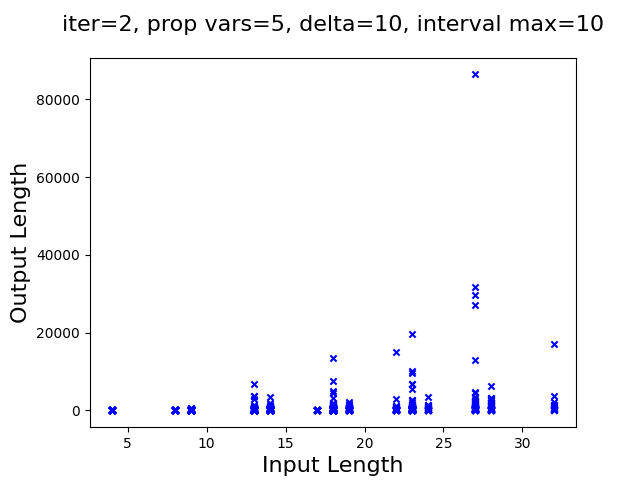
\includegraphics[scale=0.38]{images/Sim1Length_large.png}
    \captionof{figure}{Input length vs output length.\vspace{3mm}}
    \label{InputLengthVsOutputLength}
    \end{figure}
\end{minipage}
\begin{minipage}{0.5 \textwidth}
    \begin{figure}[H]
    \centering
    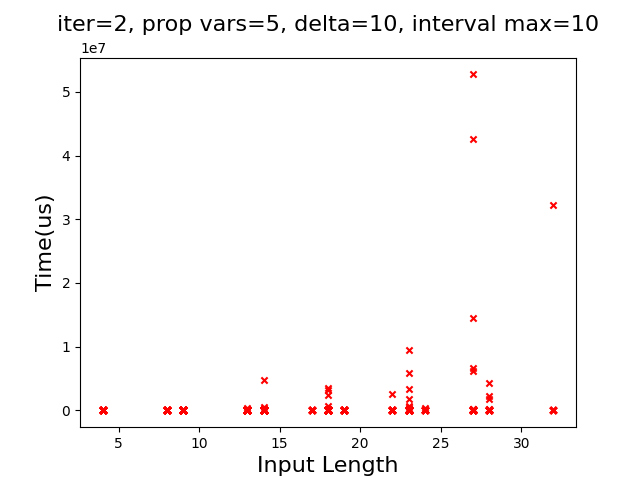
\includegraphics[scale=0.38]{images/Sim1Time_large.png}
    \captionof{figure}{Input length vs run time.\vspace{3mm}}
    \label{InputLengthVsRuntime}
    \end{figure}
\end{minipage}\\
\noindent The formula $(p_0 = p_1) \mathcal{U}_{[2,9]} (p_1 \mathcal{U}_{[7,9]} p_3)$ was an outlier for both figures, and the formulas $(p_4 \rightarrow p_2) \mathcal{R}_{[1,8]} (p_3 \mathcal{U}_{[3,4]} p_0)$ and $(p_3 \mathcal{R}_{[2,7]} p_4) \mathcal{R}_{[1,9]} (p_4 \mathcal{R}_{[4,9]} p_3)$ were outliers for Figure \ref{InputLengthVsRuntime}. \\
\noindent\textbf{Simulation 2}
For the second simulation, we consider 1 iteration, 10 propositional variables, 20 for DELTA, and 20 for INTERVAL\_MAX. Here are some examples of generated formulas:
$\mathcal{F}_{[10,17]} p_4$, $\neg p_6$, $p_6 \mathcal{U}_{[6,14]} p_8$. We obtain the following plots:\\
\begin{minipage}{0.5 \textwidth}
    \begin{figure}[H]
    \centering
    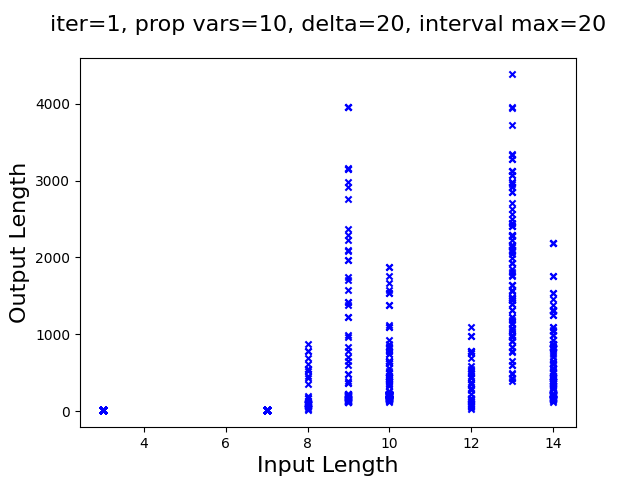
\includegraphics[scale=0.38]{images/Sim2Length_large.png}
    \captionof{figure}{Input length vs output length\vspace{3mm}}
    \label{fig:InVsOutLen}
    \end{figure}
\end{minipage}
\begin{minipage}{0.5 \textwidth}
    \begin{figure}[H]
    \centering
    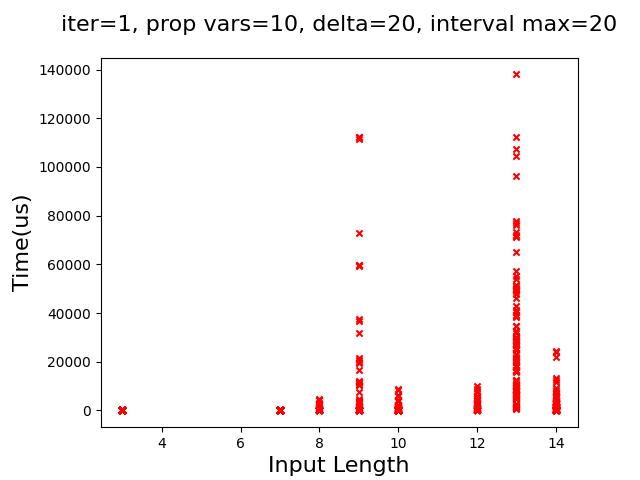
\includegraphics[scale=0.38]{images/Sim2Time_large.png}
    \captionof{figure}{Input length vs run time.\vspace{3mm}}
    \label{fig:InLenVsRunTime}
    \end{figure}
\end{minipage}\\
\noindent\textbf{Simulation 3}
For the third simulation, we consider 2 iterations, 10 propositional variables, 5 for DELTA, and 10 for INTERVAL\_MAX. We obtain the following plots:\\
\begin{minipage}{0.5 \textwidth}
    \begin{figure}[H]
    \centering
    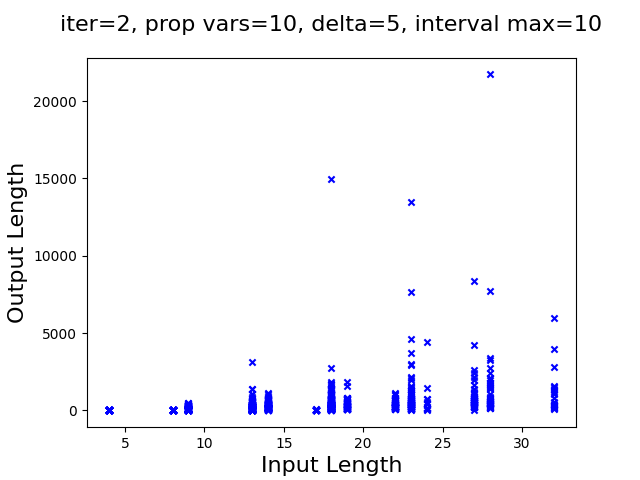
\includegraphics[scale=0.38]{images/Sim3Length_large.png}
    \captionof{figure}{Input length vs output length\vspace{3mm}}
    \label{fig:InLenVsOutLen3}
    \end{figure}
\end{minipage}
\begin{minipage}{0.5 \textwidth}
    \begin{figure}[H]
    \centering
    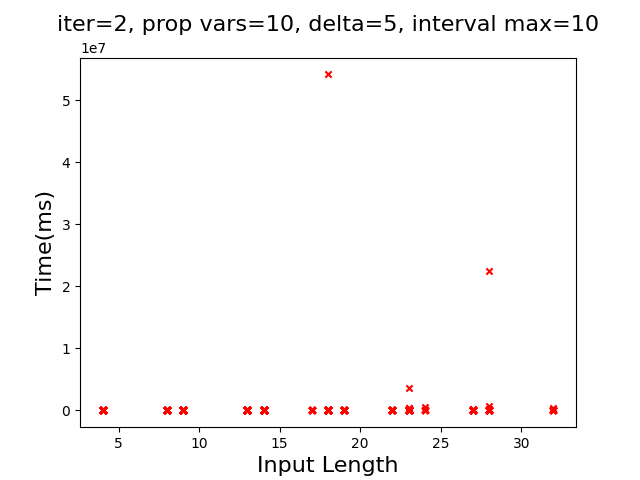
\includegraphics[scale=0.38]{images/Sim3Time_large.png}
    \captionof{figure}{Input length vs run time.\vspace{3mm}}
    \label{fig:InLenVsRunTime3}
    \end{figure}
\end{minipage}\\
The formulas $(p_7 \mathcal{U}_{[5,7]} p_9) \mathcal{U}_{[3,7]} (\mathcal{F}_{[1,4]} p_4)$ and $\mathcal{G}_{[3,7]} (p_9 \mathcal{U}_{[0,4]} p_0)$ were outliers in both figures, and Figure 5 had one more outlier from the formula $(\neg p_9) \mathcal{R}_{[5,9]} (p_5 \mathcal{U}_{[2,4]} p_3)$.
\\
\noindent\textbf{Simulation 4}
For the fourth simulation, we consider 1 iteration, 5 propositional variables, 10 for DELTA, and 10 for INTERVAL\_MAX. Some examples of generated formulas are: $\neg p_1$, $p_1 \mathcal{R}_{[6,7]} p_3$, $\mathcal{F}_{[5,5]} p_3$. We obtain the following plots:\\
\begin{minipage}{0.5 \textwidth}
    \begin{figure}[H]
    \centering
    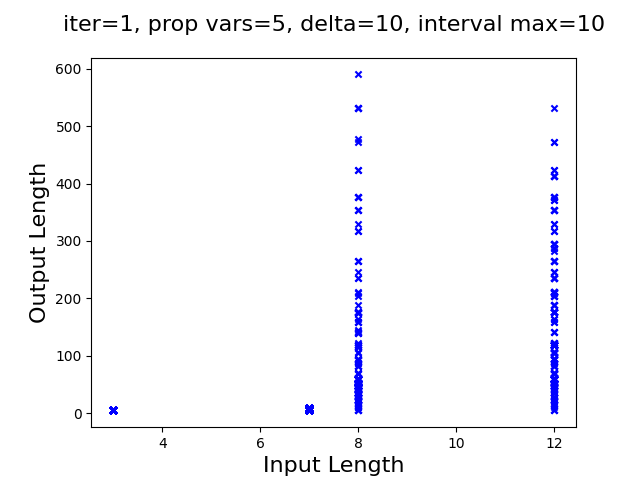
\includegraphics[scale=0.38]{images/Sim4Length_large.png}
    \captionof{figure}{Input length vs output length\vspace{3mm}}
    \label{InLenVsOutLen4}
    \end{figure}
\end{minipage}%
\begin{minipage}{0.5 \textwidth}
    \begin{figure}[H]
    \centering
    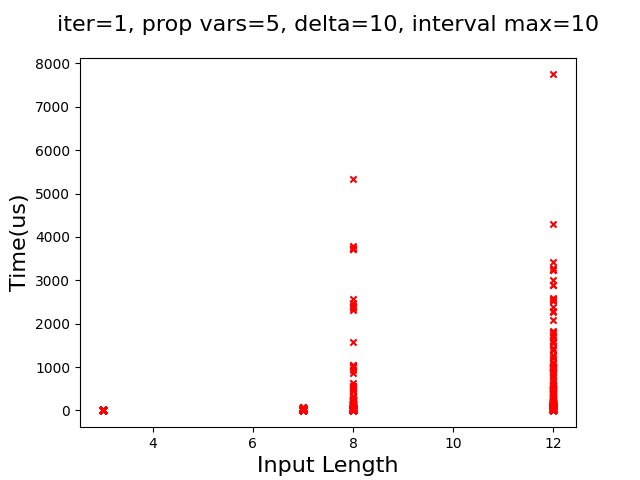
\includegraphics[scale=0.38]{images/Sim4Time_large.png}
    \captionof{figure}{Input length vs run time.\vspace{3mm}}
    \label{InLenVsRunTime4}
    \end{figure}
\end{minipage}
\noindent What we observe from the simulations is that the worst case complexity, both for space and time, is relatively rare. We also observe that these worst cases are extreme outliers and that in nearly every case, are examples of nested binary temporal operators. As seen in \cite{HLR21}, \cite{KZJZR20}, \cite{AJR22}, and \cite{HCHJR21}, nested binary temporal operators do not appear in any specifications, and thus are likely rare in practical applications.
%%%%%%%%%%%%%%%%%%%%%%%%%%%%%%%%%%%%%%%%%%%%%%%%%%
%%%%%%%%%%%%%%%%%%%%%%%%%%%%%%%%%%%%%%%%%%%%%%%%%%
\section{Correctness of WEST Tool Implementation} \label{test}
We accompany our proof of algorithmic correctness with a rigourous evaluation of implementation correctness: that our WEST tool correctly implements our WEST algorithm. % The correctness of an abstract algorithm one can describe on pencil and paper differs from the correctness of an actual implementation of the algorithm (the program). 
%On one hand, correctness of an algorithm is assured by mathematical analysis of the algorithm on all possible inputs and showing that it behaves as desired. 
%However, assuring correctness of the program is a difficult task.
Since our proof of algorithmic correctness is manual and our focus is on usability for validation by humans, we utilize more traditional techniques for robust software engineering with testing-based evaluation. An attractive alternative for future work involves encoding our proofs in an interactive theorem prover and utilizing a verified code generator like PVS2C\cite{Sha17} or the Isabelle/HOL code generator \cite{HB21}. 
Since the primary purpose of the WEST tool is valiation of formulas for humans, we focused on writing a tool with an intutiive human-facing interface then verifying that implementation rather than wrestling with verified code generated by a tool made to optimize for different objectives. 

One naive approach involves testing every possible input up to a certain size to verify the output or behaviors of the program.
For WEST, this strategy would generate a very large test suite with signficant redundancy. 
For instance, there is little sense in testing all MLTL formulas of the form $p_0 \mathcal{U}_{[0,t]} p_1$ for all $t$ such that $0 \leq t \leq 99$; verification of a few should give sufficient confidence of correctness of the program. 
We approach this problem more intelligently: we test our implementation with a test suite that explores all control paths (up to a certain depth) of the algorithm. A control path is a sequence of lines of code that are executed in one calculation of an input formula. Differing structures of formulas will lead to different sequences of lines of code to be executed, and a test suite to explore all such paths provides high confidence in the correctness of the WEST tool.

\subsection{Intelligent Fuzzing}
Negative testing is the process of checking that a program is able to handle unexpected inputs without crashing; we employ fuzz testing (also know as fuzzing), a form of negative testing.
%The earliest use of fuzzing by Miller \cite{Miller} was to discover bugs in Unix utilities by randomly generating command line inputs, and monitoring for unexpected crashes or security. This style of black box testing assumes no prior knowledge of the target program, and is centered on generating a large quantity of inputs. Miller describes his approach in \cite{Miller} as follows: \\
We deviate from traditional black-box fuzzing defined by \cite{Miller} as follows: \\
\textit{``If we consider a program to
be a complex finite state machine, then our testing strategy can be thought of as a random walk through the state space, searching for undefined states.''} \\
Instead we utilize intelligent fuzzing (sometimes referred to as whitebox fuzzing), which is an alternate approach to fuzz testing that leverages knowledge about program structure to generate valid inputs and increase coverage. 
Borrowing the words of Miller, our approach to testing the WEST program can be thought of as walking all possible paths up to a certain depth of the state space of our algorithm. 
We first outline our overall approach to intelligent fuzzing: 
\begin{enumerate}
    \item Construct a state diagram of our algorithm, represented as a directed graph. 
    The edges of the graph capture control flow of our algorithm, and vertices represent the remaining blocks of the code without branching statements.  
    \item Construct a test suite that explores all possible paths in the digraph up to a certain depth. Run the WEST program on the test suite to produce a set of output files.
    \item Run a naive brute force generator of satisfying computations on the test suite and verify that both outputs match for all test cases.
\end{enumerate}
\subsubsection{State Diagram Construction}
 We choose to represent the states space of algorithm as a directed graph with the edges representing the control flow and vertices representing blocks of contiguous code without branching statements. 
 The core of the WEST program lies in the recursive routine, \textit{reg}, which calls the $8$ different subroutines %discussed earlier,
 as shown in \ref{fig:abstracted graph}.
\begin{figure}[t]
    \centering
    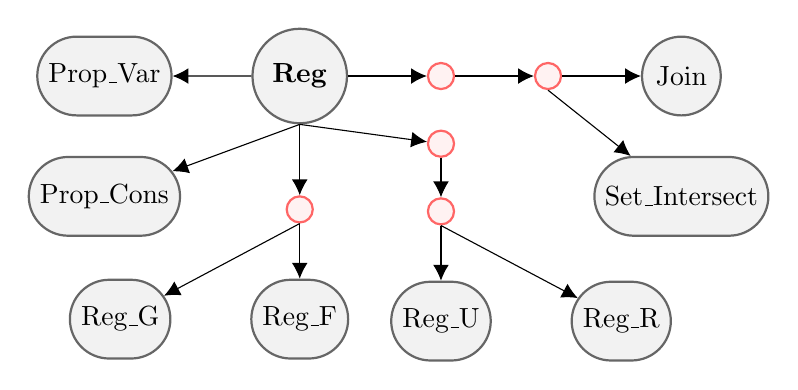
\begin{tikzpicture}[ node/.style={rounded rectangle, draw=black!60, fill=black!5, thick, minimum size=10mm},
    bignode/.style={rounded rectangle, draw=black!60, fill=black!5, thick, minimum size=12mm},
    star/.style={circle, draw=red!60, fill=red!5, thick, minimum size=1mm} ]

    %Nodes
    \node[bignode] (reg) {\textbf{Reg}};
    \node[star](prop_binary_star1)[right= of reg]{};
    \node[star](prop_binary_star2)[right= of prop_binary_star1]{};
    \node[node](join)[right=of prop_binary_star2]{Join};
    \node[node](set_intersect)[below=0.5 cm of join]{Set\_Intersect};
    \node[node] (prop_var) [left=of reg] {Prop\_Var};
    \node[node] (prop_cons) [below=0.5 cm of prop_var] {Prop\_Cons};
    \node[star](unary_star)[below=0.9 cm of reg]{};
    \node[node](reg_f)[below=0.7 cm of unary_star]{Reg\_F};
    \node[node](reg_g)[left= of reg_f]{Reg\_G};
    \node[star](temp_binary_star1)[below=0.5 cm of prop_binary_star1]{};
    \node[star](temp_binary_star2)[below=0.5 cm of temp_binary_star1]{};
    \node[node](reg_u)[below=0.7 cm of temp_binary_star2]{Reg\_U};
    \node[node](reg_r)[right=of reg_u]{Reg\_R};

    %Lines
    \draw[->] (reg.west) -- (prop_var);
    \draw[->] (reg.south) -- (prop_cons);
    \draw[->] (reg.south) -- (unary_star);
    \draw[->] (unary_star.south) -- (reg_f.north);
    \draw[->] (unary_star.south) -- (reg_g);
    \draw[->] (reg.south) -- (temp_binary_star1);
    \draw[->] (reg.east) -- (prop_binary_star1.west);
    \draw[->] (temp_binary_star1.south) -- (temp_binary_star2.north);
    \draw[->] (temp_binary_star2.south) -- (reg_r);
    \draw[->] (temp_binary_star2.south) -- (reg_u.north);
    \draw[->] (prop_binary_star1.east) -- (prop_binary_star2.west);
    \draw[->] (prop_binary_star2.east) -- (join.west);
    \draw[->] (prop_binary_star2.south) -- (set_intersect);
    \end{tikzpicture}
    
    
    
    \caption{Abstracted graph of the \textit{reg} main routine. Red nodes signal recursive calls to \textit{reg} on sub formulas of the input formula.}
    \label{fig:abstracted graph}
\end{figure}
In order to construct the intelligent fuzzing test suite, we make the design choice to abstract away the eight subroutines in the overall state space diagram, despite the fact that they may have different possible execution paths within them. Without this abstraction, attempting to explore all execution paths in this finer graph is infeasible due to the explosion in the number of paths \cite{Pham_2016}, some of which are provably impossible to construct a test input to explore.
\subsubsection{Creating the Test Suite}
 We now give the procedure of how the intelligent fuzzing test suite is generated. 
Firstly, we count the number of formulas $\phi(d)$ to be generated as a function of the exact depth $d$ of recursion desired. 
For $d = 0$, only the paths leading to \textit{prop\_var} and \textit{prop\_cons} can be explored, so $\phi(0) = 2$. For $d \geq 1$, we recursively calculate $\phi(d + 1) = 2\phi(d) + 4\phi(d)^2$; paths to \textit{reg\_G} and \textit{reg\_F} is counted in the linear term, and paths to \textit{reg\_U}, \textit{reg\_R}, \textit{set\_intersect}, and \textit{join} is counted by the quadratic term. 
This gives $\phi(1) = 20$, $\phi(2) = 1640$, and $\phi(3) = 10761680$. 
$d = 3$ is computationally infeasible, and $d = 1$ doesn't give us assurance about operators interacting with each other through nesting. Thus $d = 2$ is a happy medium. 
The full test suite is generated in a similar recursive manner. 
Firstly, the $d = 0$ test suite comprises of two formulas: a propositional variable or its negation, and a propositional constant. 
Then for any $d \geq 1$, the test suite is constructed by iterating through all formulas in the depth $d-1$ test suite for \textit{reg\_G} and \textit{reg\_F}, and all pairs of formulas from the $d-1$ test suite for the remaining four recursive paths. 
To ensure wider coverage, each of the propositional variables or their negation and propositional constants are randomly generated.
\subsubsection{Verifying against Naive Brute Force}
 A relatively straight forward approach to generating the set of all satisfying computations of a MLTL formula $\phi$ over $n$ variables, such that $m = \text{cplen}(\phi)$, is to iterate over all $2^{m \cdot n}$ possible computations, which counts all possible length $m \cdot n$ bit strings. 
The main work is done by an interpreter function that takes arguments of computation $\pi$ and MLTL formula $\phi$ and determines if $\pi \vDash \phi$ purely based on semantics that define MLTL.
Every first-order quantifier is easily translated to loops, and checking for satisfying conditions of the suffix of a computation naturally lends itself to recursion.
The full implementation details can be found on the %\href{https://github.com/zwang271/2022-Iowa-State-REU-Temporal-Logic-.git} %KYR: blind review
{GitHub} repository. 
As expected for a brute force implementation, extensive run time poses a major limitation; the previously mentioned infeasibility of not abstracting away subroutines and running test suites for deeper depths is primarily caused by this stage of verification. 
On an Intel(R) Core(TM) i7-4770S CPU at 3.10GHz with 32gb RAM, the brute force program took nearly nine hours to execute the depth two test suite of $1640$ formulas. 
For this test suite, the number of propositional variables was fixed at $n = 4$ and the largest computation length was $m = 5$, from formulas with doubly-nested temporal operators. 
In comparison, the WEST program executed the same test suite in under thirty minutes on the same machine. One thing to note is that the brute force program outputs only computations of zeros and ones, and thus comparing the outputs of the WEST program requires expanding out the `$S$' characters in the regular expressions. For instance, the regular expression ``$1SS0SS1$" yields $2^{\text{\# of `$S$'s}} = 2^4 = 16$ computations after expansion.
It's important to state that although the full test suite matches between both implementations, absolute correctness on all inputs is not guaranteed for either program. However, the successful execution of the test suite gives us a much higher confidence in correctness of both the WEST program and the brute force program. 
%%%%%%%%%%%%%%%%%%%%%%%%%%%%%%%%%%%%%%%%%%%%%%%%%%
%%%%%%%%%%%%%%%%%%%%%%%%%%%%%%%%%%%%%%%%%%%%%%%%%%
\section{Regular Expression Simplification Theorem} \label{simpsection}
 As a final result of our paper, we provide a regular expression simplification theorem. This theorem describes a form of a set of computations that are guaranteed to simplify down to a string of all `$S$'s. Although not implemented in the WEST program, this theorem may help users identify tautologies, as the WEST program does not always output a single string of `$S$'s when a formula holds true for every computation. We first define some vocabulary.\\
 We say a regular expression composed entirely of `$S$'s and commas is an \emph{arbitrary computation}. For the purposes of the following theorem, we remove all commas from computations. We say `0' or a `1' in a regular expression is a \emph{fixed truth value}. We overload the definition of a matrix and say that a \emph{matrix} is a representation of a union of regular expressions, where each row is a regular expression. This aids significantly in the description and proof of the theorem; note, however, that matrix algebra does not apply in this definition. 
\begin{theorem}[\emph{Regular Expression Simplification Theorem}] \label{simp}
Let M be a $n+1$ by $n$ matrix, where each of the $n+1$ rows represents a regular expression of length n with commas stripped. If each column has one `$1$', one `$0$', and $n-1$ `$S$'s, then the union of this set of regular expressions can be simplified to $S^n$, the arbitrary computation of length $n$.
\end{theorem}
Note that this theorem gives us a sufficient but not a necessary condition for simplification to the arbitrary computation. One such example is the regular expression $101|S1S|1S0|0SS$, which fails the hypothesis of the  simplification theorem but is still equivalent to $SSS$.
\subsection{Implementation Challenges of the Regular Expression Simplification Theorem}
First, the proof of our algorithm relies on a set of $n+1$ regular expressions, yet it is obvious that the inclusion of redundant regular expressions of the same computation length in the union wouldn't alter this equivalence. A program implementation of this theorem would require an algorithm to parse through and identify which of these regular expressions are redundant and don't match the format of those described in our proof.

\begin{figure}[h!]
\begin{minipage}{.62\textwidth}
\begin{example} \label{example1}
Consider the MLTL formula:
$T \ \mathcal{U_{[\text{0,3}]}} p_0 = \mathcal{F_{[\text{0,3}]}}p_0$.
The WEST program outputs a union of regular expressions represented by the matrix in \eqref{matrix_ex3}. Instances like this demonstrate the utility of the regular expression simplification theorem; a recursive function implementation of this theorem would simplify output to the arbitrary computation. However, we foresee some challenges to the implementation of this algorithm.
\end{example}
\end{minipage}
\begin{minipage}{.38\textwidth}
%     \noindent \textbf{Example:}
    % \vspace{-0.05\textwidth}
\begin{equation} \label{matrix_ex3}
    \begin{pmatrix}
    1 & S & S & S\\
    S & 1 & S & S\\
    S & S & 1 & S\\
    S & S & S & 1\\
    0 & 0 & 0 & 0
    \end{pmatrix}
\end{equation}
\end{minipage}
\end{figure}

For example, adding the row ``$1,1,1,1$" to the matrix generated by example \ref{example1} would change the matrix to not match the specifications of the theorem, but the union would still simplify to the arbitrary computation. Next, it is possible that a regular expression could be appended with a substring of `$S$'s at the beginning or end.

\begin{figure}[h!]
\begin{minipage}{.62\textwidth}
\begin{example} \label{example2}
Consider the following MLTL formula: $T \ \mathcal{U_{[\text{2,3}]}} p_0 \equiv \mathcal{F_{[\text{2,3}]}}p_0$. The WEST program generates a union of regular expressions corresponding to the matrix shown in \eqref{matrix_ex4}. It can clearly be seen that this is equivalent to the arbitrary computation, as one can remove the first two columns and apply the simplification theorem to the remaining columns.
\end{example}
\end{minipage}
\begin{minipage}{.38\textwidth}
\begin{equation} \label{matrix_ex4}
    \begin{pmatrix}
      S & S & 1 & S \\
      S & S & S & 1 \\
      S & S & 0 & 0
    \end{pmatrix}
\end{equation}
\end{minipage}
\end{figure}

Furthermore, identical substrings may be interspersed throughout the set of regular expressions. Then, the union of them won't simplify to the arbitrary computation, but rather, the arbitrary computation ``broken up" by common substrings. Consider the following modification to the matrix generated by example \ref{example1}:\\
\begin{minipage}{.5\textwidth}
The substrings ``$0$", ``$1S0$", and ``$1$" are inserted at the beginning, middle, and end, respectively. In general, a vector of length $m$ strings seeking to apply the theorem to $n$ of its columns has $m \choose n$ combinations of columns to check for. Implementation of this algorithm can drastically increase run-time while proving its utility in only a small number of circumstances.
\end{minipage}
\begin{minipage}{.5\textwidth}
\begin{center}
$
\begin{pmatrix}
  0 & \mathbf{1} & \mathbf{S} & 1 & S & 0 & \mathbf{S} & \mathbf{S} & 1\\
  0 & \mathbf{S} & \mathbf{1} & 1 & S & 0 & \mathbf{S} & \mathbf{S} & 1\\
  0 & \mathbf{S} & \mathbf{S} & 1 & S & 0 & \mathbf{1} & \mathbf{S} & 1\\
  0 & \mathbf{S} & \mathbf{S} & 1 & S & 0 & \mathbf{S} & \mathbf{1} & 1\\
  0 & \mathbf{0} & \mathbf{0} & 1 & S & 0 & \mathbf{0} & \mathbf{0} & 1\\
    \end{pmatrix} 
    \vspace{2mm}
    \equiv  0\mathbf{S}\mathbf{S}1S0  \mathbf{S}\mathbf{S}1
$
\end{center}
\end{minipage}
%%%%%%%%%%%%%%%%%%%%%%%%%%%%%%%%%%%%%%%%%%%%%%%%%%
%%%%%%%%%%%%%%%%%%%%%%%%%%%%%%%%%%%%%%%%%%%%%%%%%%
\section{Closing Remarks}
\label{Conclusion}
 One goal of this research project is to visually represent MLTL formulas as truth tables, similar to classical truth tables in propositional logic. 
The goal is motivated by the fact that MLTL is widely used in industry by engineers and scientists to write specifications for safe critical systems, and the WEST program can aide in the debugging of such specifications. 
The WEST program accomplishes this: given MLTL formula $\phi$, we compute a way to capture all satisfying formulas $\pi$ in a relatively readable format that additionally captures structural patterns in such regular expressions. 
The tool itself has demonstratively reasonable run time. 
Although worst case theoretical complexity is doubly exponential, our benchmarking shows that the most severe case is very sparse in practice. 
We have also applied techniques in intelligent fuzzing to explore the state space of the algorithm in a structured way. 
For a reasonably complex program, a complete walk of the input space is infeasible. 
However, basing testing on a (manually constructed) graph of the algorithm provides a middle ground where some level of coverage is guaranteed. 
Although this isn't a magic box that generates test cases for arbitrary algorithms, the methods used in algorithmic analysis and test suite construction are easily adaptable to similar recursive algorithms.
\subsection{Additional Research Directions}
\textbf{Describe all satisfying computations to LTL formulas using $\omega$-regular expressions.}
$\omega$-regular expression are defined to match only infinite words, and can be used to describe satisfying computations to LTL formulas (which has infinite time steps). 
Our original efforts were spent reasoning about the general LTL case before restricting to MLTL. Particular difficulties revolves around the need for the Kleene star operation, which leads to messy arithmetic of infinite unions and intersections of regular expressions. \\
\noindent \textbf{Simplifying unions of regular expressions to a minimal representation.}
Theorem \ref{simp} addresses a non-trivial situation in which a vector of regular expressions may be simplified. A natural question to ask is what is the minimum number of strings of regular expressions needed to represent a language of computations. However, such a minimal representation is not unique. For instance, $\mathscr{L}(S1|1S) = \mathscr{L}(S1|10) = \{01, 10, 11\}$. There may be other schemes needed to simplify any arbitrary union of regular expressions to their minimal representation.\\
\noindent \textbf{A more general application of intelligent fuzzing to recursive algorithms.}
A tool to systematically convert a recursive algorithm (perhaps written in some strictly defined pseudocode syntax) into a directed graph representation of the state space would be a helpful aid for generating test suites. 
Significant efforts were made to construct the graph of the WEST algorithm by hand, and an automated process would invaluable. 
Additional care should be put into allowing for varying levels of abstractions of execution due to concerns of the path explosion problem. 
% FUTURE WORK:
% potentially recursive function implementation of Regular Expression Simplification Theorem
%% \subsubsection{Acknowledgements}
%% \hspace{\parindent} This work was done as part of Iowa State University's Research Experience for Undergraduates funded by NSF grant DMS-1950583. We would like to thank Iowa State University and the NSF for this research opportunity.
%% The assistance of our mentors Dr. Kristin Yvonne Rozier and Laura Gamboa Guzmán was invaluable and greatly appreciated. In addition, we thank Dr. Steve Butler and Dr. Bernard Lidický for their management of this program and organization of its funding.
%% Finally, we want to thank Brian Kempa for his guidance and suggestions on the intelligent fuzzing portion of our research, and Dr. Steve Butler for his intuition on the Regular Expression Simplification Theorem.
%
% ---- Bibliography ----
%
% BibTeX users should specify bibliography style 'splncs04'.
% References will then be sorted and formatted in the correct style.
%
\bibliographystyle{splncs04}
\bibliography{Citations}
\newpage
%%%%%%%%%%%%%%%%%%%%%%%%%%%%%%%%%%%%%%%%%%%%%%%%%%
%%%%%%%%%%%%%%%%%%%%%%%%%%%%%%%%%%%%%%%%%%%%%%%%%%
\appendix
\section*{Appendix} \label{Appendix}
\renewcommand{\thesection}{\Roman{section}}
Content in the appendices will appear online, on the paper's website, but appears here for now due to blind review.

 \section{Soundness and Completeness} \label{Appendix-SoundComplete}
%  \vspace{-0.1in}
 We write $\mathscr{L}(\text{reg}(\phi))$ to denote the language of reg($\phi$). That is, the set of computations represented by the regular expression $\text{reg}(\phi)$.

 %KYR: TODO: label this theorem 2!!!!!!!!!!!!!!!!!!!!!!
 \begin{theorem}[\emph{Soundness and Completeness}]
 For any well formed MLTL formula $\phi$ in negation normal form, a computation $\pi$ with $|\pi| = \text{cplen}(\phi)$ satisfies $\phi$ and  if and only if $\pi \in \mathscr{L}(\emph{reg}(\phi))$.
 \end{theorem}
 \begin{proof}
 We proceed by induction on the length of the formula.\\
 
 \noindent \textbf{Base Cases.}\\
 \noindent\textbf{reg($\top$)}\\
 Any computation $\pi$ satisfies $\top$, and $\mathscr{L}(\text{reg}(\top))$ is the set of all computations of one time step. Padding conventions extends this to the set of all computations of any positive number of time steps, so we are done.\\
 
 \noindent\textbf{reg($\bot$)}\\
 There are no computations that satisfy $\bot$ and $\mathscr{L}(\text{reg}(\bot))$ is the empty string, so we are done.\\
 
 \noindent\textbf{reg($p_k$)}\\
 For $0\leq k \leq n-1$, consider the propositional variable $p_k$. If $\pi$ satisfies $p_k$, then $p_k$ evaluates to true at $\pi[0]$. This is equivalent to writing that $\pi[0]$ is of the form 
 $$S^{k} 1 S^{n-k-1}$$
 which is precisely reg($p_k$).\\
 
 \noindent\textbf{reg($\neg p_k$)}\\
 If $\pi$ satisfies $\neg p_k$, then $\neg p_k$ evaluates to true at $\pi[0]$. This is equivalent to writing that $\pi[0]$ is of the form 
 $$S^{k} 0 S^{n-k-1}$$
 which is precisely reg($\neg p_k$).\\
 
 \noindent\textbf{Inductive Step.}\\
 Suppose the theorem holds for MLTL formulas $\varphi$ and $\psi$. We now show that it holds for $\varphi \land \psi$, $\varphi \lor \psi$, $\mathcal{F}_{[a,b]} \varphi$, $\mathcal{G}_{[a,b]} \varphi$, $\varphi \ \mathcal{U}_{[a,b]} \psi$, and $\varphi \mathcal{R}_{[a,b]} \psi$.\\
 
 \noindent \textbf{reg($\varphi \land \psi$)}\\
 We know that $\pi \vDash \varphi \land \psi \text{ iff } \pi \vDash \varphi \text{ and } \pi \vDash \psi$.\\
 By the inductive hypothesis, $\pi \vDash \varphi$ iff $\pi \in \mathscr{L}(\text{reg}(\varphi))$ and 
 \\$\pi \vDash \psi$ iff $\pi \in \mathscr{L}(\text{reg}(\psi))$, so
 $$\pi \vDash \varphi \land \psi \text{ iff } \pi \in (\mathscr{L}(\text{reg}(\varphi)) \land \mathscr{L}(\text{reg}(\psi))) = \mathscr{L}(\text{reg}(\varphi \land \psi)).$$
 
 \noindent \textbf{reg($\varphi \lor \psi$)}\\
 We know that $\pi \vDash \varphi \lor \psi \text{ iff } \pi \vDash \varphi \text{ or } \pi \vDash \psi$.\\
 By the inductive hypothesis, $\pi \vDash \varphi$ iff $\pi \in \mathscr{L}(\text{reg}(\varphi))$ and 
 \\$\pi \vDash \psi$ iff $\pi \in \mathscr{L}(\text{reg}(\psi))$, so
 $$\pi \vDash \varphi \lor \psi \text{ iff } \pi \in (\mathscr{L}(\text{reg}(\varphi)) \lor \mathscr{L}(\text{reg}(\psi))) = \mathscr{L}(\text{reg}(\varphi \lor \psi)).$$
 
 \noindent \textbf{reg($\mathcal{F}_{[a,b]} \varphi$)}\\
 We know that $\pi \vDash \mathcal{F}_{[a,b]} \varphi \text{ iff } |\pi| > a \text{ and } \exists i \in [a,b] \text{ such that } \pi_i \vDash \varphi$.\\
 If $|\pi| = \text{cplen}(\mathcal{F}_{[a,b]} \varphi)$, $|\pi| > a$. Likewise, $\pi \in \mathscr{L}\left(\text{reg}\left(\mathcal{F}_{[a,b]} \varphi \right)\right)$ implies $|\pi| = \text{cplen}(\mathcal{F}_{[a,b]} \varphi)$, so the length condition is satisfied.\\
 By the inductive hypothesis, $\pi_i \vDash \varphi$ iff $\pi_i \in \mathscr{L}(\text{reg}(\varphi))$, so $\pi \in \mathscr{L}((S^n,)^i \text{reg}(\varphi))$ for some $i \in [a,b]$. Equivalently, 
 $$\pi \in \mathscr{L}\left(\bigvee_{i=a}^{b} (S^n,)^i \text{reg}(\phi)(,S^n)^{b-i}\right) = \mathscr{L}(\text{reg}(\mathcal{F}_{[a,b]}\varphi)).$$

 \noindent \textbf{reg($\mathcal{G}_{[a,b]} \varphi$)}\\
 We know that $\pi \vDash \mathcal{G}_{[a,b]}\varphi \text{ iff } |\pi| \leq a \text{ or } \forall i \in [a,b] \ \pi_i \vDash \varphi$.\\
 Since $|\pi| = \text{cplen}(\mathcal{G}_{[a,b]} \varphi)$ and $\text{cplen}(\mathcal{G}_{[a,b]} \varphi) > a$, the first option for satisfying the formula never occurs.\\
 By the inductive hypothesis, $\pi_i \vDash \varphi$ iff $\pi_i \in \mathscr{L}(\text{reg}(\varphi))$, so $\pi \in \mathscr{L}((S^n,)^i \text{reg}(\varphi))$ for all $i \in [a,b]$. Equivalently, 
 $$\pi \in \mathscr{L}\left(\bigwedge_{i=a}^{b} (S^n,)^i \text{reg}(\phi)(,S^n)^{b-i}\right) = \mathscr{L}(\text{reg}(\mathcal{F}_{[a,b]}\varphi)).$$
 
 \noindent \textbf{reg($\varphi \ \mathcal{U}_{[a,b]} \psi$)}\\
  We have that 
  $$\pi \vDash \varphi \ \mathcal{U}_{[a,b]} \psi \text{ iff } |\pi| > a \text{ and } \exists i \in [a,b] \text{ such that } (\pi_i \vDash \psi \text{ and } \forall a \leq j < i, \pi_j \vDash \varphi).$$
  As argued in the Finally case, the length condition is satisfied.\\
  By the inductive hypothesis, $\pi_i \vDash \psi$ iff $\pi_i \in \mathscr{L}(\text{reg}(\psi))$, or equivalently, \\
  $\pi \in \mathscr{L}(\text{reg}(\mathcal{G}_{[i,i]} \psi))$. Also, $\pi_j \vDash \varphi$ if and only if $\pi_j \in \mathscr{L}(\text{reg}(\varphi))$.\\
  By the argument used in the Global case, we see that $\forall a \leq j < i, \ \pi_j \vDash \varphi$ is equivalent to $\pi \in \mathscr{L}(\text{reg}(\mathcal{G}_{[a, i-1]} \varphi))$.\\
  Thus $\pi \vDash \varphi \ \mathcal{U}_{[a,b]} \psi$ iff $\pi \in \mathscr{L}((\text{reg}(\mathcal{G}_{[i,i]} \psi) \land \text{reg}( \mathcal{G}_{[a, i-1]} \varphi)))$ for some $i \in [a,b]$, or equivalently, 
  $$\pi \in \mathscr{L}\left(\bigvee_{i=a}^{b} \text{reg}\left(\mathcal{G}_{[a,i-1]}\phi \land \mathcal{G}_{[i, i]} \psi\right)\right) = \mathscr{L}\left(\text{reg}(\varphi \ \mathcal{U}_{[a,b]} \psi)\right).$$
  
  \noindent \textbf{reg($\varphi \mathcal{R}_{[a,b]} \psi$)}\\
  We have that
  \begin{align*}
    &\pi \vDash \varphi \mathcal{R}_{[a,b]} \psi \text{ iff } |\pi| \leq a \text{ or } \forall i \in [a,b] \ \pi_i \vDash \psi \text{ or } \\ 
    &\exists j\in[a,b] \text{ such that }
    (\pi_j \vDash \varphi \text{ and } \forall a\leq k \leq j, \pi_k \vDash \psi).
  \end{align*}
  As argued in the Global case, the first option for satisfying the formula never occurs.\\
  By the Global case, the statement $\forall i\in[a,b] \ \pi_i \vDash \psi$ is equivalent to $\pi \in \mathscr{L}(\text{reg}(\mathcal{G}_{[a,b]} \psi))$ and, by the Finally case. the statement $\exists j\in[a,b]$ such that ($\pi_j \vDash \varphi$ and $\forall a\leq k \leq j$, $\pi_k \vDash \psi$) is equivalent to $\pi \in \mathscr{L}\left(\bigvee_{i=a}^{b} \text{reg}\left(\mathcal{G}_{[a,i]}\psi \land \mathcal{G}_{[i, i]} \phi\right)\right)$. Hence 
  
  \begin{align*}
    \pi \vDash \varphi \mathcal{R}_{[a,b]} \psi \text{ iff } \pi &\in \mathscr{L}\left(\text{reg}(\mathcal{G}_{[a,b]} \psi) \lor \bigvee_{i=a}^{b} \text{reg}\left(\mathcal{G}_{[a,i]}\psi \land \mathcal{G}_{[i, i]} \phi\right)\right) \\
    &= \mathscr{L}\left(\text{reg}(\mathcal{G}_{[a,b]} \psi) \lor \bigvee_{i=a}^{b-1} \text{reg}\left(\mathcal{G}_{[a,i]}\psi \land \mathcal{G}_{[i, i]} \phi\right)\right)\\
    &= \mathscr{L}\left(\text{reg}(\varphi \mathcal{R}_{[a,b]} \psi)\right).
  \end{align*}
  
 \noindent This completes the inductive step, and thus the proof. Since this proof addresses all possible MLTL formulas in negation normal form, it shows completeness along with soundness.
 \end{proof}
% \newpage


 %%%%%%%%%%%%%%%%%%%%%%%%%%%%%%%%%%%%%%%%%%%%%%%%%%%%%%%%%%%%%%%%%%%%%
 %%%%%%%%%%%%%%%%%%%%%%%%%%%%%%%%%%%%%%%%%%%%%%%%%%%%%%%%%%%%%%%%%%%%%
\section{Nested Until and Release Rewriting Theorem} \label{Appendix-NestedUR}

 \begin{theorem}[\emph{Nested Until and Release Rewriting Theorem}] \label{NestedUR}
   Any MLTL formula using the Until or Release operator can be rewritten with right-nested subformulas. Let $\mathcal{B} = \mathcal{R} \text{ or } \mathcal{U}$. Let $a,b,c \in \mathbb{Z}_{\geq 0} , a \leq b,$ \text{and} $ \phi,   \psi$ \text{be well-formed MLTL formulas in NNF. Then,} $ \phi \ \mathcal{B}_{[a,b+c]} \psi = \phi \ \mathcal{B}_{[a,b]}(\phi \ \mathcal{B}_{[0,c]} \psi)$. That is, $ \phi \ \mathcal{U}_{[a,b+c]} \psi \equiv \phi \ \mathcal{U}_{[a,b]}(\phi \ \mathcal{U}_{[0,c]} \psi)$ and $ \phi \ \mathcal{R}_{[a,b+c]} \psi \equiv \phi \ \mathcal{R}_{[a,b]}(\phi \ \mathcal{R}_{[0,c]} \psi)$.
\end{theorem}
The proof of Theorem \ref{NestedUR} appears below.


%KYR: this totally goes here in the journal version but in an appendix/on a website for the conference version

\begin{proof}

\textbf{Case 1: $\mathbf{\mathcal{B} = \mathcal{U}}$}\\

\noindent Let $\gamma = \phi \ \mathcal{U}_{[0,c]} \psi$. Then, $\phi \ \mathcal{U}_{[a,b]}(\phi \ \mathcal{U}_{[0,c]} \psi) = \phi \ \mathcal{U}_{[a,b]}\gamma$ and $\text{reg}\left(\gamma\right) = \bigvee_{j=0}^{c} \text{reg}\left(\mathcal{G}_{[0,j-1]}\phi \land \mathcal{G}_{[j, j]}\psi\right).$ Thus

\begin{align*}
\text{reg}\left(\phi \ \mathcal{U}_{[a,b]}\gamma\right) &= \bigvee_{i=a}^{b} \text{reg}\left(\mathcal{G}_{[a,i-1]}\phi \land \mathcal{G}_{[i, i]}\text{reg}\left(\gamma\right)\right)\\
&= \bigvee_{i=a}^{b} \text{reg}\left(\mathcal{G}_{[a,i-1]}\phi \land  \mathcal{G}_{[i, i]}\left( \bigvee_{j=0}^{c} \text{reg}\left(\mathcal{G}_{[0,j-1]}\phi\right) \land \text{reg}\left(\mathcal{G}_{[j, j]}\psi\right) \right) \right).
\end{align*}
$\mathcal{G}_{[i, i]}$ distributes over $\land$ and $\lor$, so
\begin{align*}
\text{reg}\left(\phi \ \mathcal{U}_{[a,b]}\gamma\right) &= \bigvee_{i=a}^{b} \text{reg}\left(\mathcal{G}_{[a,i-1]}\phi \land  \bigvee_{j=0}^{c} \mathcal{G}_{[i, i]}\left( \text{reg}\left(\mathcal{G}_{[0,j-1]}\phi\right) \land \text{reg}\left(\mathcal{G}_{[j, j]}\psi\right) \right) \right) \\
&= \bigvee_{i=a}^{b} \text{reg}\left(\mathcal{G}_{[a,i-1]}\phi \land \left( \bigvee_{j=0}^{c} \mathcal{G}_{[i, i]}\text{reg}\left(\mathcal{G}_{[0,j-1]}\phi\right) \land \mathcal{G}_{[i, i]}\text{reg}\left(
\mathcal{G}_{[j, j]}\psi \right) \right) \right).
\end{align*}
Since $\mathcal{G}_{[t_1,t_1]} \mathcal{G}_{[t_2,t_3]} \phi \equiv \mathcal{G}_{[t_1+t_2,t_1+t_3]} \phi$, we have
\begin{align*}
\text{reg}\left(\phi \ \mathcal{U}_{[a,b]}\gamma\right) &= \bigvee_{i=a}^{b} \text{reg}\left(\mathcal{G}_{[a,i-1]}\phi \land \left( \bigvee_{j=0}^{c} \text{reg}\left(\mathcal{G}_{[i,i+j-1]}\phi\right) \land \text{reg}\left(\mathcal{G}_{[i+j, i+j]}\psi \right) \right) \right) \\
&= \bigvee_{i=a}^{b}  \bigvee_{j=0}^{c} \text{reg}\left(\mathcal{G}_{[a,i-1]}\phi\right) \land  \text{reg}\left(\mathcal{G}_{[i,i+j-1]}\phi\right) \land \text{reg}\left(\mathcal{G}_{[i+j, i+j]}\psi \right).
\end{align*}
Since $\mathcal{G}_{[t_1,t_2-1]}\phi \land \mathcal{G}_{[t_2,t_3]} \phi \equiv \mathcal{G}_{[t_1,t_3]} \phi$, we have
\begin{align*}
\text{reg}\left(\phi \ \mathcal{U}_{[a,b]}\gamma\right) &= \bigvee_{i=a}^{b}  \bigvee_{j=0}^{c} \text{reg}\left(\mathcal{G}_{[a,i+j-1]}\phi\right) \land \text{reg}\left(\mathcal{G}_{[i+j, i+j]}\psi  \right)\\
&= \bigvee_{i+j=a}^{b+c} \text{reg}\left(\mathcal{G}_{[a,i+j-1]}\phi\right) \land \text{reg}\left(\mathcal{G}_{[i+j, i+j]}\psi  \right).
\end{align*}
Finally, let $k = i + j$. Thus
\begin{align*}
\text{reg}\left(\phi \ \mathcal{U}_{[a,b]}\gamma\right) &= \bigvee_{k=a}^{b+c} \text{reg}\left(\mathcal{G}_{[a,k-1]}\phi\right) \land \text{reg}\left(\mathcal{G}_{[k, k]}\psi  \right) \\
&= \text{reg}\left(\phi \ \mathcal{U}_{[a,b+c]} \psi\right).
\end{align*}
This shows that $\phi \ \mathcal{U}_{[a,b]}(\phi \ \mathcal{U}_{[0,c]} \psi) \equiv \phi \ \mathcal{U}_{[a,b+c]} \psi$.\\

\noindent \textbf{Case 2: $\mathbf{\mathcal{B} = \mathcal{R}}$} \\
We begin by rewriting the regex for Release in an equivalent form to better mirror the structure of the Until case. The Release operator is the dual of the Until operator. Thus,  \\
\begin{align*}
\text{reg}\left(\phi \ \mathcal{R}_{[a,b]}\psi\right) &= \text{reg}\left(\neg\left(\neg\phi \ \mathcal{U}_{[a,b]}\neg\psi\right)\right) \\
&= \neg\left(\bigvee_{i=a}^{b} \text{reg}\left(\mathcal{G}_{[a,i-1]}\neg\phi \land \mathcal{G}_{[i, i]}\neg\psi\right)\right).
\end{align*}
Global is the dual of Finally, so
\begin{align*}
\text{reg}\left(\phi \ \mathcal{R}_{[a,b]}\psi\right) &= \neg\left(\bigvee_{i=a}^{b} \text{reg}\left(\neg\mathcal{F}_{[a,i-1]}\phi \land \neg\mathcal{F}_{[i, i]}\psi\right)\right)\\
&= \neg\left(\bigvee_{i=a}^{b} \text{reg}\left(\neg\left(\mathcal{F}_{[a,i-1]}\phi \lor \mathcal{F}_{[i, i]}\psi\right)\right)\right)\\
&= \neg\neg\left(\bigwedge_{i=a}^{b} \text{reg}\left(\mathcal{F}_{[a,i-1]}\phi \lor \mathcal{F}_{[i, i]}\psi\right)\right)\\
&= \bigwedge_{i=a}^{b} \text{reg}\left(\mathcal{F}_{[a,i-1]}\phi \lor \mathcal{F}_{[i, i]}\psi\right).
\end{align*}
This completes the rewriting of the regex for Release. Now let $\gamma = \phi \ \mathcal{R}_{[0,c]} \psi$. Then $\phi \ \mathcal{R}_{[a,b]}(\phi \ \mathcal{R}_{[0,c]} \psi) = \phi \ \mathcal{R}_{[a,b]}\gamma$ and
$\text{reg}\left(\gamma\right) = \bigwedge_{j=0}^{c} \text{reg}\left(\mathcal{F}_{[0,j-1]}\phi \lor \mathcal{F}_{[j, j]}\psi\right)$. Thus
\begin{align*}
\text{reg}\left(\phi \ \mathcal{R}_{[a,b]}\gamma\right) &= \bigwedge_{i=a}^{b} \text{reg}\left(\mathcal{F}_{[a,i-1]}\phi \lor \mathcal{F}_{[i, i]}\text{reg}\left(\gamma\right)\right)\\
&= \bigwedge_{i=a}^{b} \text{reg}\left(\mathcal{F}_{[a,i-1]}\phi \lor  \mathcal{F}_{[i, i]}\left( \bigwedge_{j=0}^{c} \text{reg}\left(\mathcal{F}_{[0,j-1]}\phi\right) \lor \text{reg}\left(\mathcal{F}_{[j, j]}\psi\right) \right) \right).
\end{align*}
$\mathcal{F}_{[i, i]} \equiv \mathcal{G}_{[i, i]}$, so this operation distributes over $\land$ and $\lor$. Thus
\begin{align*}
\text{reg}\left(\phi \ \mathcal{R}_{[a,b]}\gamma\right) &= \bigwedge_{i=a}^{b} \text{reg}\left(\mathcal{F}_{[a,i-1]}\phi \lor  \bigwedge_{j=0}^{c} \mathcal{F}_{[i, i]}\left( \text{reg}\left(\mathcal{F}_{[0,j-1]}\phi\right) \lor \text{reg}\left(\mathcal{F}_{[j, j]}\psi\right) \right) \right) \\
&= \bigwedge_{i=a}^{b} \text{reg}\left(\mathcal{F}_{[a,i-1]}\phi \lor \left( \bigwedge_{j=0}^{c} \mathcal{F}_{[i, i]}\text{reg}\left(\mathcal{F}_{[0,j-1]}\phi\right) \lor \mathcal{F}_{[i, i]}\text{reg}\left(\mathcal{F}_{[j, j]}\psi \right) \right) \right).
\end{align*}
Since $\mathcal{F}_{[t_1,t_1]}\mathcal{F}_{[t_2,t_3]} \phi \equiv \mathcal{F}_{[t_1+t_2,t_1+t_3]} \phi$, we have
\begin{align*}
\text{reg}\left(\phi \ \mathcal{R}_{[a,b]}\gamma\right) &= \bigwedge_{i=a}^{b} \text{reg}\left(\mathcal{F}_{[a,i-1]}\phi \lor \left( \bigwedge_{j=0}^{c} \text{reg}\left(\mathcal{F}_{[i,i+j-1]}\phi\right) \lor \text{reg}\left(\mathcal{F}_{[i+j, i+j]}\psi \right) \right) \right) \\
&= \bigwedge_{i=a}^{b}  \bigwedge_{j=0}^{c} \text{reg}\left(\mathcal{F}_{[a,i-1]}\phi\right) \lor  \text{reg}\left(\mathcal{F}_{[i,i+j-1]}\phi\right) \lor \text{reg}\left(\mathcal{F}_{[i+j, i+j]}\psi \right).
\end{align*}
Since $\mathcal{F}_{[t_1,t_2-1]} \phi \land \mathcal{F}_{[t_2,t_3]} \phi \equiv \mathcal{F}_{[t_1, t_3]} \phi$, we have
\begin{align*}
\text{reg}\left(\phi \ \mathcal{R}_{[a,b]}\gamma\right) &= \bigwedge_{i=a}^{b}  \bigwedge_{j=0}^{c} \text{reg}\left(\mathcal{F}_{[a,i+j-1]}\phi\right) \lor \text{reg}\left(\mathcal{F}_{[i+j, i+j]}\psi  \right) \\
&= \bigwedge_{i+j=a}^{b+c} \text{reg}\left(\mathcal{F}_{[a,i+j-1]}\phi\right) \lor \text{reg}\left(\mathcal{F}_{[i+j, i+j]}\psi  \right).
\end{align*}
Let $k = i + j$. Thus
\begin{align*}
\text{reg}\left(\phi \ \mathcal{R}_{[a,b]}\gamma\right) &= \bigwedge_{k=a}^{b+c} \text{reg}\left(\mathcal{F}_{[a,k-1]}\phi\right) \lor \text{reg}\left(\mathcal{F}_{[k, k]}\psi  \right) \\
&= \text{reg}\left(\phi \ \mathcal{R}_{[a,b+c]} \psi\right).
\end{align*}
Thus  $\phi \ \mathcal{R}_{[a,b]}(\phi \ \mathcal{R}_{[0,c]} \psi) \equiv \phi \ \mathcal{R}_{[a,b+c]} \psi$, so $\phi \ \mathcal{B}_{[a,b+c]} \psi \equiv \phi \ \mathcal{B}_{[a,b]}(\phi \ \mathcal{B}_{[0,c]} \psi)$. This completes the proof.
\end{proof}


 
%%%%%%%%%%%%%%%%%%%%%%%%%%%%%%%%%%%%%%%%%%%%%%%%%%
%%%%%%%%%%%%%%%%%%%%%%%%%%%%%%%%%%%%%%%%%%%%%%%%%%

 \section{Until and Release Duality Lemma} \label{duality appendix}
 \begin{lemma}[\emph{Until and Release Duality}]\label{dual_proof}
 The definition of Release is equivalent to the dual of Until: 
 $\phi \mathcal{R} \psi \equiv \neg (\neg \phi \mathcal{U} \neg \psi)$. That is to say,
$\phi \mathcal{R}_{[a,b]} \psi$ if and only if $|\pi| \le a \text{ or } \forall s \in [a,b] ,(\pi_s \vDash \psi \text{ or } \exists t \in [a, s-1] , \pi_t \vDash \phi)$.
 \end{lemma}
 
\begin{proof} $ $\newline
($\Rightarrow$):\\
\indent Suppose $\pi \vDash \phi \mathcal{R}_{[a,b]} \psi$, so:
\[ |\pi| \leq a \text{ or } \forall i \in [a,b] \text{, (} \pi_i \vDash \psi \text{) or } \exists j \in [a,b-1] \text{, (} \pi_j \vDash \phi \text{ and } \forall k \in [a, j] \pi_k \vDash \psi \text{)} \]
We proceed by cases to show that:
\[
|\pi| \le a \text{ or } \forall s \in [a,b] \text{, (} \pi_s \vDash \psi \text{ or } \exists t \in [a, s-1] \text{, } \pi_t \vDash \phi \text{)} \tag{A1}
\]
\indent Case 0: If $|\pi| \leq a$, then we are immediately done.
\indent Case 1: Suppose $\forall i \in [a,b] \text{, } \pi_i \vDash \psi$.\\
\indent Through re-labeling, we have $\forall s \in [a,b] \text{, } \pi_s \vDash \psi$. Then we clearly have:
\[
|\pi| \le a \text{ or } \forall s \in [a,b] \text{, (} \pi_s \vDash \psi \text{ or } \exists t \in [a, s-1] \text{, } \pi_t \vDash \phi \text{)} \tag{A1}
\]
\indent Case 2: Suppose $\exists i \in [a,b] \text{, } \pi_i \cancel{\vDash} \psi$.\\
\indent \indent Then we must have that:
\[ \exists j \in [a,b-1] \text{, (} \pi_j \vDash \phi \text{ and } \forall k \in [a, j] \ \pi_k \vDash \psi \text{)} \tag{1} \]
\indent \indent We want to show that $ \forall s \in [a,b] \text{, (} \exists t \in [a, s-1] \text{, } \pi_t \vDash \phi \text{)}$.\\
\\
\indent \indent Suppose by contradiction that: 
\[ \exists s \in [a,b] \text{, (} \forall t \in [a, s-1] \text{, } \pi_t \cancel{\vDash} \phi \text{)} \tag{2} \]
\indent \indent Since $s \in [a,b] \text{ and }  t \in [a, s-1]$, we have that $t \in [a,b-1]$.\\
\indent \indent Since $j \in [a,b-1]$ (from Line 1), we have that $\pi_j \cancel{\vDash} \phi$ from Line 2.\\
\indent \indent However from Line 1 we have that $\pi_j \vDash \phi$ and have thus derived a contradiction.\\
\indent \indent Thus, we now have that $ \forall s \in [a,b] \text{, (} \exists t \in [a, s-1] \text{, } \pi_t \vDash \phi \text{)}$.\\ \indent \indent From this, we clearly have that:
\[
|\pi| \le a \text{ or } \forall s \in [a,b] \text{, (} \pi_s \vDash \psi \text{ or } \exists t \in [a, s-1] \text{, } \pi_t \vDash \phi \text{)} \tag{A1}
\]
$ $ \newline
\indent Since these $3$ cases exhaustively capture all cases fo the assumption, the ($\Rightarrow$) direction is proved.
$ $ \newline
\noindent ($\Leftarrow$):\\
\indent Suppose that $\pi \vDash \neg (\neg \phi \mathcal{U} \neg \psi)$:
\[
|\pi| \le a \text{ or } \forall s \in [a,b] \text{, (} \pi_s \vDash \psi \text{ or } \exists t \in [a, s-1] \text{, } \pi_t \vDash \phi \text{) \tag{1}}
\]
$ $ \newline
\indent We want to show $\pi \vDash \phi R_{[a,b]} \psi$, that is:
\[ |\pi| \leq a \text{ or } \forall i \in [a,b] \text{, (} \pi_i \vDash \psi \text{) or } \exists j \in [a,b-1] \text{, (} \pi_j \vDash \phi \text{ and } \forall k \in [a, j] \ \pi_k \vDash \psi \text{)} \tag{B1} \]
\indent Case 0: If $|\pi| \leq a$, again we are immediately done. \\
\indent Case 1: Suppose $\forall s \in [a,b] \text{, (} \pi_s \vDash \psi \text{)}$.\\ 
\indent \indent Relabeling $s$ to $i$, we now have that $\forall i \in [a, b] \text{, (}\pi_s \vDash \psi \text{)}$, which implies line B1. \\
\indent Case 2: Suppose $\exists s \in [a,b], \pi_s \cancel{\vDash} \psi$.\\
\indent \indent By re-labeling $s$ to $i$, we have that $\exists i \in [a,b], \pi_i \cancel{\vDash} \psi$.\\
\indent \indent Since $[a,b]$ is a finite-discrete interval, there must exist a first $i_1$ s.t. $\pi_{i_1} \cancel{\vDash} \psi$, that is:
\[ 
\exists i_1 \in [a,b]\text{, (}  \pi_{i_1} \cancel{\vDash} \psi  \text{ and }  \forall k \in [a, i_1 - 1] \text{, } \pi_{k} \vDash \psi \text{)}
\tag{2}\]
\indent \indent Since (line 2) $\exists i_1 \in [a,b], \pi_{i_1} \cancel{\vDash} \psi$, by Line 1 we have that: $\pi_{i_1} \vDash \psi \text{ or } \exists t \in [a, i_1 - 1] \text{, } \pi_t \vDash \phi$.\\
\indent \indent Thus, we have that: 
\[
\exists t \in [a, i_1 - 1] \text{, } \pi_t \vDash \phi \tag{3}
\]
\indent \indent Since  $[a, t] \subseteq [a, i_1 - 1]$ and $\forall k \in [a, i_1 - 1] \text{, } \pi_{k} \vDash \psi$, we have that:
\[ 
\forall k \in [a, t]\text{, } \pi_{k} \vDash \psi \tag{4}
\]
\indent \indent Since $[a,t] \subseteq [a, i_1 - 1] \subseteq [a,b-1]$, we have that $t \in [a,b-1]$, so let $j := t$.
\indent \indent Then from lines 3 and 4, we have that:
\[
\exists j \in [a,b-1] \text{, (} \pi_j \vDash \phi \text{ and } \forall k \in [a, j] \ \pi_k \vDash \psi \text{)} \tag{5}
\]
\indent \indent From line 5, we now get:
\[ 
|\pi| \leq a \text{ or } \forall i \in [a,b] \text{, (} \pi_i \vDash \psi \text{) or } \exists j \in [a,b-1] \text{, (} \pi_j \vDash \phi \text{ and } \forall k \in [a, j] \ \pi_k \vDash \psi \text{)} \tag{B1}
\]
\indent Again the 3 cases are exhaustive of all cases in the assumption, this we have the ($\Leftarrow$) direction.\\
\\
This finishes the proof.
\end{proof}
%%%%%%%%%%%%%%%%%%%%%%%%%%%%%%%%%%%%%%%%%%%%%%%%%%
%%%%%%%%%%%%%%%%%%%%%%%%%%%%%%%%%%%%%%%%%%%%%%%%%%
\section{Regular Expression Simplification Theorem} \label{simp appendix}
\begin{proof}[Proof of \ref{simp}]
Assume no row is the arbitrary computation, because then the union of the set of regular expressions would trivially simplify to the arbitrary computation.\\
We begin by showing that there must be at least one row in the matrix $M$ that is composed of one fixed truth value and $n-1$ `$S$'s. This will be of use later in the proof. Because there are $n$ columns and $2$ fixed truth values in each column, there are $2n$ fixed truth values. There are $n+1$ rows, so the average number of fixed truth values per row is strictly less than $2$ since $\frac{2n}{n+1} < \ 2$.
Thus, there must exist at least one row composed of one fixed truth value and $n-1$ `$S$'s. \\
\noindent We now proceed by induction on the length of computations, $n$. \\
\textbf{Base Cases:} $n=1$ and $n=2$. \\
The $n=1$ case holds by definition:
    $$\begin{bmatrix}
    1\\
    0
    \end{bmatrix}  \equiv S.$$
For $n=2$, we can manually verify that each possible matrix indeed satisfies the theorem. Note that because the union of regular expressions is commutative, any permutation of rows is equivalent:
        $$\begin{bmatrix}
    1 & S\\
    S & 1\\
    0 & 0
    \end{bmatrix}  \equiv \begin{bmatrix}
    0 & S\\
    S & 0\\
    1 & 1
    \end{bmatrix} \equiv \begin{bmatrix}
    1 & S\\
    S & 0\\
    0 & 1
    \end{bmatrix} \equiv \begin{bmatrix}
    0 & S\\
    S & 1\\
    1 & 0
    \end{bmatrix} \equiv SS.
        $$
\noindent \textbf{Inductive Hypothesis:}\\
Let $n\geq 2$. Assume that a matrix of regular expressions, $H$, with the following characteristics is equivalent to the arbitrary computation of length $n-1$: $n$ rows, $n-1$ columns, one `$1$' per column, one `$0$' per column, and $n-2$ `$S$'s per column.\\
\noindent \textbf{Inductive Step:}\\
Consider a matrix of regular expressions, $J$, with the following characteristics: $n+1$ rows, $n$ columns, one `$1$' per column, one `$0$' per column, and $n-1$ `$S$'s per column. We show $J$ is equivalent to the arbitrary computation of length $n$.\\
As aforementioned, there must exist at least one row composed of one fixed truth value and $n-1$ `$S$'s, and the union of regular expressions is commutative. Thus, WLOG, let the first row of $J$, $r_1$, be a row with one known truth value.
Suppose this known truth value is in column $k$, $c_k$, where $1 \leq k \leq n$.. Assume WLOG that this value is a 0. Matrix $J$ can be represented as follows:
\[
J = \begin{blockarray}{cccccccc}
\mathbf{c_1} & & \mathbf{c_{k-1}} & \mathbf{c_k} & \mathbf{c_{k+1}} & & \mathbf{c_n} \\
\begin{block}{(ccccccc)c}
    S & \hdots & S & 0 & S & \hdots & S & \mathbf{r_1}\\
     &  &  & S &  &  &  & \mathbf{r_2}\\
    &  &  & \vdots &  &  &  & \\
    &  & & S &  &  &  & \\
    & \vdots &  & 1 &  & \vdots &  & \\
    & &  & S &  & &  & \\
    &  &  & \vdots & &  &  & \\
    &  & & S & &  & & \mathbf{r_{n+1}}\\
\end{block}
\end{blockarray}
 \]
The first row of $J$ represents half of the regular expressions contained in the arbitrary computation. The other half would be represented by a regular expression of all `S's, except for a `1' at the $k^{th}$ position. Thus, if the rest of $J$, rows $r_2$ through $r_{n+1}$, represents the other half of the arbitrary computation, then the matrix - the union of the set of the regular expressions - represents the arbitrary computation of length $n$. We show that this is indeed the case:
Because the first row represents all the computations with `0' at the $k^{th}$ position, every `$S$' in $c_k$ can be replaced with a `1', to avoid redundancy; the case for which each `$S_k$' is `0' is a subset of $r_1$. Thus, matrix $J$ can be represented as follows:
\[
J = \begin{blockarray}{cccccccc}
\mathbf{c_1} & & \mathbf{c_{k-1}} & \mathbf{c_k} & \mathbf{c_{k+1}} & & \mathbf{c_n} \\
\begin{block}{(ccccccc)c}
    S & \hdots & S & 0 & S & \hdots & S & \mathbf{r_1}\\
     &  &  & 1 &  &  &  & \mathbf{r_2}\\
    &  \vdots &  & \vdots &  &  \vdots &  & \\
    &  &  &  &  & &  & \\
    & & & 1 & &  & & \mathbf{r_{n+1}}\\
\end{block}
\end{blockarray}
 \]
The problem reduces to showing that $J - r_1$, that is, $J$ with the row $r_1$ removed, represents the other half of the arbitrary computation. Thus, let $J' = J - r_1$:
\[
J' = \begin{blockarray}{cccccc}
\mathbf{c_1} &  & \mathbf{c_k} & & \mathbf{c_n} \\
\begin{block}{(ccccc)c}
     &   & 1 &   &  & \mathbf{r_2}\\
     \vdots & &  \vdots & & \vdots  & \\
    &   &   & &  & \\
    & & 1 &  & & \mathbf{r_{n+1}}\\
\end{block}
\end{blockarray}
 \]
Again, we want to show that $J'$ represents the other half of the arbitrary computation. Recall that we specify this to be the union of regular expressions of all $`S'$s except for a $`1'$ at the $k^{th}$ position. Because each row indeed contains a $`1'$ at the $k^{th}$ position, the problem reduces to showing that $r_2 - c_k$ through $r_{n+1} - c_k$ represents the arbitrary computation, where $r_j - c_k$ is the row $r_j$ with the $k^{th}$ entry removed. Thus, we remove $c_k$ from $J'$ and call this new matrix $J''$:
\[
 J'' = \begin{pmatrix}
    r_2 - c_k \\
    . \\
    . \\
    . \\
    r_{n+1} - c_k \\
    
  \end{pmatrix}
\]
Because $J''$ is the result removing one row and one column from $J$, $J''$ has $n$ rows and $n-1$ columns. In each column of $J''$, there remains one `$1$' and one `$0$'. Also, there are now $n-2$ `$S$'s in each column, because $r_1$ was removed. Thus, $J''$ is equivalent to $H$, and is therefore equivalent to the arbitrary computation by the inductive hypothesis.
Because $r_1$ is equivalent to half of the arbitrary computation and $J'$ is equivalent to the other half of the arbitrary computation, $J$ is equivalent to the arbitrary computation, as the union of $r_1$ and $J'$ is equivalent to $J$.
Therefore, by induction, the theorem holds.
\end{proof}
%%%%%%%%%%%%%%%%%%%%%%%%%%%%%%%%%%%%%%%%%%%%%%%%%%
%%%%%%%%%%%%%%%%%%%%%%%%%%%%%%%%%%%%%%%%%%%%%%%%%%
\section{Pseudocode for the WEST Algorithm Functions} \label{pseudocode appendix}
 
To compute the satisfying computations of an MLTL formula, many of the functions in the WEST program require the regular expressions of the satisfying computations of the subformulas as inputs. We denote these regexes by $R$ and $T$, where $R = R_1 | R_2 | ... | R_k$ is represented as a vector of strings $R = {R_1, R_2, ..., R_k}$, and $T = T_1 | T_2 | ... | T_\ell$ is represented as a vector of strings $T = {T_1, T_2, ..., T_\ell}$. Additionally, $n$ will always refer to the number of propositional variables, and nnf refers to an input formula in negation normal form.
\begin{algorithm}[H]
\caption{Pad a vector to elements of all equal length}
%Input: Vector of strings that represents a regex, number of propositional variables \\
%Output: Vector of strings padded to equal length
\begin{algorithmic}
\Procedure{Pad}{vector $R$, int $n$} 
    \State max\_Length $\leftarrow$ $\max_{\{r \in R\}}$($r$.length())
    \For{($r \in R$)}
        \State diff $\leftarrow$ (max\_length$- r$.length()) / $(n+1)$ 
        \State  $r \leftarrow r + (,S^n)^{\text{diff}}$
    \EndFor
    \State return $R$
    
\EndProcedure
\end{algorithmic}
\end{algorithm}
\begin{algorithm}[H]
\caption{Computes regex for propositional constant}
%Input: String that is either ``T" or ``!", number of propositional variables\\
%Output: Vector of strings that represents the appropriate satisfying computations
\begin{algorithmic}
\Procedure{reg\_prop\_cons}{string nnf, int $n$}
    \If {(nnf $=$ ``T" and $n \neq 0$)} return $\{S^n\}$
    \Else \hspace{1mm} return $\{\}$ 
    \EndIf
\EndProcedure
\end{algorithmic}
\end{algorithm}
\begin{algorithm}[H]
\caption{Output the vector of computation satisfying a propositional variable.}
%Input: String that represents a propositional variable or the negation of one, number of propositional variables \\
%Output: Vector of strings that represents the appropriate satisfying computations
\begin{algorithmic}
\Procedure{reg\_prop\_var}{string nnf, int $n$}
    \If {(nnf $=$ ``p$k$", where $k$ is a nonnegative integer)} return $\{S^k1S^{n-k-1}\}$
    \EndIf 
    \If {(nnf $=$ ``$\scriptstyle{\sim}$p$k$", where $k$ is a nonnegative integer)} return $\{S^k0S^{n-k-1}\}$
    \EndIf
\EndProcedure
\end{algorithmic}
\end{algorithm}
\begin{algorithm}[H]
\caption{Combines two strings that differ only by one character into one}
%Input: Two strings that represent regexes\\
%Output: Single string that represents computations represented by both input strings or FAIL
\begin{algorithmic}
\Procedure{simplify\_string}{string $r$, string $t$}   
    \If{($r$.length() $\neq$ $t$.length())} exit
        \EndIf
    \For{($0 \leq i < r$.length())}
        \State pre\_r $\leftarrow r[0, i-1]$ 
        \State char\_r $\leftarrow r[i]$ 
        \State post\_r $\leftarrow r[i+1, r\text{.length()}-1]$ 
        \State pre\_t $\leftarrow t[0, i-1]$ 
        \State char\_t $\leftarrow t[i]$ 
        \State post\_t $\leftarrow t[i+1, t\text{.length()}-1]$
        \If{(pre\_r $=$ pre\_t and post\_r $=$ post\_t)}
            \If{(char\_r $\neq$ char\_t)}
                \State return pre\_r +``$S$" + post\_r 
            \Else
                \State return $r$
            \EndIf
        \EndIf
    \EndFor
    \State return FAIL 
\EndProcedure
\end{algorithmic}
\end{algorithm}
 
\begin{algorithm}[H]
\caption{Simplifies a vector of strings using simplify\_string}
%Input: Vector of strings representing a regex\\
%Output: Vector of strings representing a regex simplified using simplify\_string
\begin{algorithmic}
\Procedure{simplify}{vector $R$}    
    \State Pad all strings in $R$ to the same length
    \If{($R$.length() $\leq 1$)} return $R$
        \EndIf
    \State $i = R\text{.length} - 1$
    \State $j = i - 1$
    
    \State START
    \While{($i \geq 1$)}
        \While{($j \geq 0$)}
            \State simplified = simplify\_string($R[i]$, $R[j]$) 
            \If{(simplified $\neq$ FAIL)}
                \State replace string at index $j$ with simplified
                \State remove string at index $i$ from $R$
                \State $i = R\text{.length()} - 1$
                \State $j = i - 1$
                \State goto START
                \EndIf
            \State -{}-$j$
            \EndWhile
        \State -{}-$i$
        \State $j = i - 1$
        \EndWhile
        
    \State return $R$
\EndProcedure
\end{algorithmic}
\end{algorithm}
\begin{algorithm}[H]
\caption{Takes the intersection of two computations}
%Input: Two strings representing regexes\\
%Output: Bitwise AND of the inputted strings
\begin{algorithmic}
\Procedure{bit\_wise\_and}{string $r$, string $t$}
    \State ret $\leftarrow$ ``" 
    \For {(i $\in [0, \ r\text{.length()}]$)}
        \If{($r[i] \land$ $t[i] = ``"$)} return ``"
        \Else \hspace{1mm} ret $\leftarrow$ ret $+$ $r[i] \land t[i]$
        \EndIf
    \EndFor
    \State return ret
\EndProcedure
\end{algorithmic}
\end{algorithm}

\begin{algorithm}[H]
\caption{Takes union of two regexes (combines two vectors into one)}
%Input: Vectors of strings that represent regexes, simplify boolean\\
%Output: Vector of strings that represents union of inputted regexes
\begin{algorithmic}
\Procedure{join}{vector $R$, vector $T$, bool simp}
    \State ret $\leftarrow \{\}$
    \For{($r \in R$)} add $r$ to ret
    \EndFor
    \For{($t \in T$)} add $t$ to ret
    \EndFor
    \If{(simp is true)} return simplify(ret)
    \Else \hspace{1mm}return ret
    \EndIf
\EndProcedure
\end{algorithmic}
\end{algorithm}
\begin{algorithm}[H]
\caption{Computes the regex for a MLTL formula F[a:b]$\phi$}
% Inputs: Vector of strings representing the regex for $\phi$, interval bounds, number of propositional variables, simplify boolean\\
% Output: Vector of strings that represents the appropriate satisfying computations 
\begin{algorithmic}
\Procedure{reg\_F}{vector reg\_phi, int $a$, int $b$, int $n$, bool simp} 
    \State pre $\leftarrow$ ((`$S$')$^{n}$ + `,')$^{a}$
    \State comp $\leftarrow$ reg\_phi
    \If{$a > b$} return $\{\}$
    \EndIf
    \For{($1 \leq i \leq b-a$) }
        \State temp\_phi $\leftarrow$ ((`$S$')$^{n}$ + `,')$^{i}$ + reg\_phi
        \State comp $\leftarrow$ join(comp, temp\_phi, simp)
    \EndFor
    \State return pre + comp
\EndProcedure
\end{algorithmic}
\end{algorithm}
\begin{algorithm}[H]
\caption{Computes the regex for a MLTL formula G[a:b]$\phi$}
%Inputs: Vector of strings representing the regex for $\phi$, interval bounds, number of propositional variables, simplify boolean\\
%Output: Vector of strings that represents the appropriate satisfying computations
\begin{algorithmic}
\Procedure{reg\_G}{vector reg\_phi, int $a$, int $b$, int $n$, bool simp} 
    \State pre $\leftarrow$ ((`$S$')$^{n}$ + `,')$^{a}$
    \State comp $\leftarrow$ reg\_phi 
    \If{$a > b$} return $\{S^n\}$
    \EndIf
    \For{($1 \leq i \leq b-a$)}
        \State temp\_phi $\leftarrow$ ((`$S$')$^{n}$ + `,')$^{i}$ + reg\_phi
        \State comp $\leftarrow$ set\_intersect(comp, temp\_phi, simp)
    \EndFor
    \State return pre + comp
\EndProcedure
\end{algorithmic}
\end{algorithm}
\begin{algorithm}[H]
\caption{Computes the regex for a MLTL formula $\phi$R[a:b]$\psi$}
%Inputs: Vectors of strings representing the regexes for $\phi$ and $\psi$, interval bounds, number of propositional variables, simplify boolean\\
%Output: Vector of strings that represents the appropriate satisfying computations 
\begin{algorithmic}
\Procedure{reg\_R}{vector reg\_phi, vector reg\_psi, int $a$, int $b$, int $n$, bool simp} 
    \State comp $\leftarrow$ reg\_G(reg\_psi, $a$, $b$, $n$, simp)
    \If{$a > b$} return $\{S^n\}$
    \EndIf
    \For{($a \leq i \leq b-1$) }
        \State temp\_comp $\leftarrow$ set\_intersect(reg\_G(reg\_psi, $a$, $i$, $n$), reg\_G(reg\_phi, $i$, $i$, $n$), $n$, simp)
        \State comp $\leftarrow$ join(comp, temp\_comp, simp)
    \EndFor
    \State return comp
\EndProcedure
\end{algorithmic}
\end{algorithm}
\begin{algorithm}[H]
    \caption{Generates test suite template without propositional constants, propositional variables, or negations of propositional variables filled in}
    %Inputs: Depth of desired test suite template to generate, interval bounds\\
    %Output: Vector of MLTL formulas (without propositional constants, propositional variables, or negations of propositional variables)
    \begin{algorithmic}
        \Procedure{generate\_test\_template}{int depth, int $a$, int $b$}
        \If{(depth = 0)} return $\{p, q\}$
        \EndIf
        \State template $\leftarrow \{\}$
        \State $V \leftarrow$ generate\_test\_template(depth$- 1$, $a$, $b$)
        \For{(string $\phi \in V$)}
            \State add ``G[a:b]" + $\phi$ to template
            \State add ``F[a:b]" + $\phi$ to template
            \For{string $\psi \in V$}
                \State add $\phi$ + ``U[a:b]" + $\psi$ to template
                \State add  $\phi$ + ``R[a:b]" + $\psi$ to template
                \State add $\phi$ + ``$\lor$" + $\psi$ to template
                \State add $\phi$ + ``\&" + $\psi$ to template
            \EndFor
        \EndFor
        \State return template
    \EndProcedure
    \end{algorithmic}
    
\end{algorithm}
\begin{algorithm}[H]
    \caption{Generates a complete test suite of MLTL formulas in negation normal form up to a certain depth}
    %Inputs: Depth of desired test suite template to generate, interval bounds, number of propositional variables\\
    %Output: Vector of MLTL formulas
    \begin{algorithmic}
        \Procedure{generate\_test}{int depth, int $a$, int $b$, int $n$}
        \State tests $\leftarrow$ generate\_test\_template(depth, $a$, $b$) 
        \For{string $t \in $ tests}
            \For{char ch $\in t$}
                \If{ch $ = p$}
                    \State $k \leftarrow \text{rand()} \% n$ 
                    \If{rand() $\% 2 = 0$} replace ch with p$k$
                    \Else \hspace{1mm}replace ch with $\scriptstyle{\sim}$p$k$
                    \EndIf
                \ElsIf{ch $= q$}
                    \If{rand() $\% 2 = 0$} replace ch with T
                    \Else \hspace{1mm}replace ch with $!$
                    \EndIf
                \EndIf
            \EndFor
        \EndFor
    \State return tests
    \EndProcedure
    \end{algorithmic}
\end{algorithm}
%%%%%%%%%%%%%%%%%%%%%%%%%%%%%%%%%%%%%%%%%%%%%%%%%%
%%%%%%%%%%%%%%%%%%%%%%%%%%%%%%%%%%%%%%%%%%%%%%%%%%
\section{State Diagram Graphs} \label{graphs appendix}
\vspace{-1.5cm}
Below we provide the state diagram graphs of the functions examined in our intelligent fuzzing. Nodes in the graph represent portions of the code without control flow statements, so a single node can represent large chunks of code. Directed edges represent branching of control flow, such as IF statements and loops. Each graph directly corresponds with the pseudocode of their corresponding function, with nodes and edges being labeled accordingly. Note that the option to run \textit{simplify} has been omitted for clarity.\\

\begin{minipage}{0.4\textwidth}
\begin{figure}[H]
    \centering
    \resizebox{7cm}{!}{
    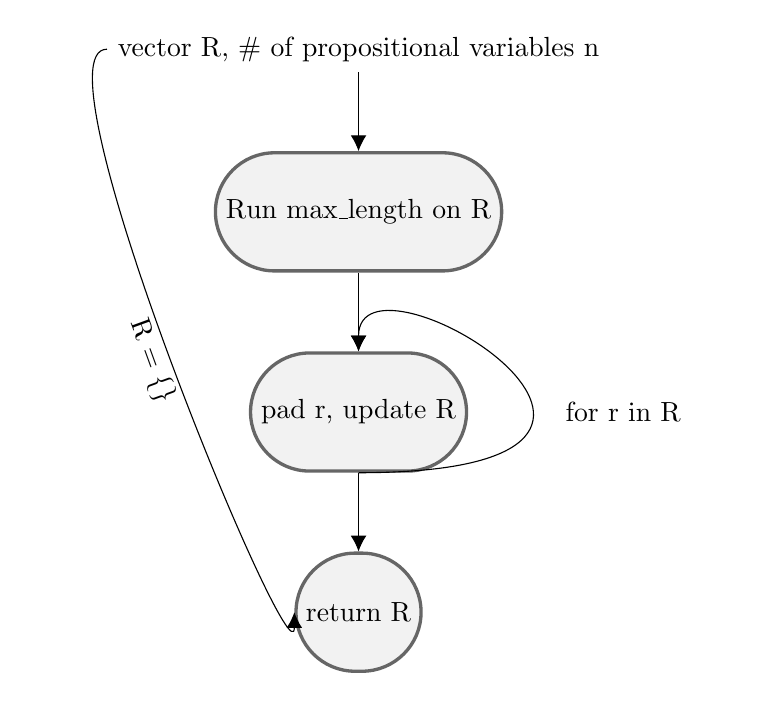
\begin{tikzpicture}[node/.style={rounded rectangle, draw=black!60, fill=black!5, very thick, minimum size=15mm}, bignode/.style={rounded rectangle, draw=black!60, fill=black!5, very thick, minimum size=20mm}, emptynode/.style={draw=none, fill=none, very thick, minimum size=1mm}]
    
    %Nodes
    \node[emptynode](inputs){vector R, \# of propositional variables n};
    \node[node](length)[below=of inputs]{Run max\_length on R};
    \node[node](body)[below=of length]{pad r, update R};
    \node[emptynode](empty_vector)[rotate=-70, left=1cm of body]{R $=\{\}$};
    \node[emptynode](for_loop)[right=1.1cm of body]{for r in R};
    \node[node](return)[below=of body]{return R};
    
    %Lines
    \draw[->] (inputs.south) -- (length.north);
    \draw[->] (length.south) -- (body.north);
    \draw[->] (body.south) -- (return.north);
    \draw[->] (inputs.west) .. controls +(left:1 cm) and +(down:1 cm) .. (return.west);
    \draw[->] (body.south) .. controls +(right:5 cm) and +(up:1.5 cm) .. (body.north);
    
    \end{tikzpicture}
    }
    \caption{Pad Function}
    \label{fig:pad graph}
\end{figure}
\end{minipage}
\begin{minipage}{0.5\textwidth}
\begin{figure}[H]
    \centering
    \resizebox{8.5cm}{!}{
    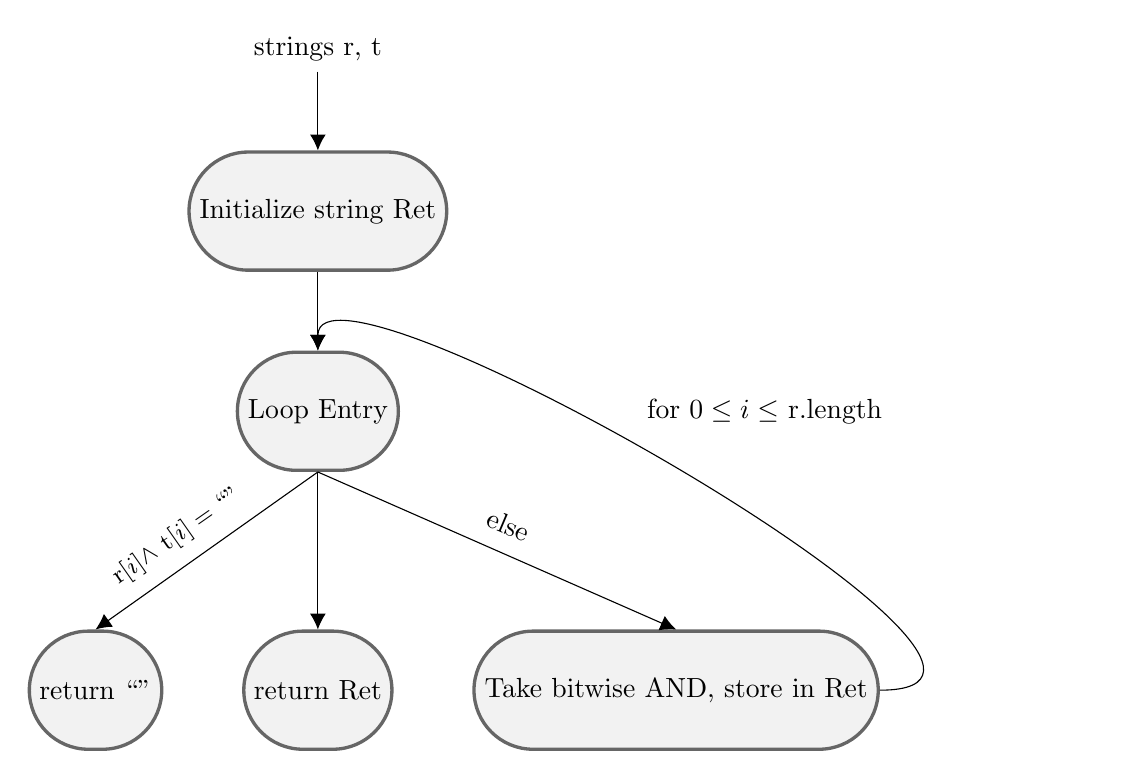
\begin{tikzpicture}[node/.style={rounded rectangle, draw=black!60, fill=black!5, very thick, minimum size=15mm}, bignode/.style={rounded rectangle, draw=black!60, fill=black!5, very thick, minimum size=20mm}, emptynode/.style={draw=none, fill=none, very thick, minimum size=1mm}]
    
    %Nodes
    \node[emptynode](inputs){strings r, t};
    \node[node](initialize)[below=of inputs]{Initialize string Ret};
    \node[node](loop_entry)[below=of initialize]{Loop Entry};
    \node[node](return)[below=2cm of loop_entry]{return Ret};
    \node[node](empty)[left=of return]{return ``"};
    \node[node](update)[right=of return]{Take bitwise AND, store in Ret};
    \node[emptynode](placeholder)[below=0.05cm of loop_entry]{};
    \node[emptynode](emptytext)[rotate=35, left=.75cm of placeholder]{\small{r$[i] \land$ t$[i] = ``"$}};
    \node[emptynode](placeholder2)[below=0.05cm of placeholder]{};
    \node[emptynode](else)[rotate=-23, right=1.9cm of placeholder2]{else};
    \node[emptynode](updatetext)[right=3cm of loop_entry]{for $0 \leq i \leq$ r.length};
    
    %Lines
    \draw[->] (inputs.south) -- (initialize.north);
    \draw[->] (initialize.south) -- (loop_entry.north);
    \draw[->] (loop_entry.south) -- (return.north);
    \draw[->] (loop_entry.south) -- (empty.north);
    \draw[->] (loop_entry.south) -- (update.north);
    \draw[->] (update.east) .. controls +(right:3 cm) and +(up:1.5 cm) .. (loop_entry.north);
    
    \end{tikzpicture}
    }
    \caption{Bitwise\_And Function}
    \label{fig:bitwise_and graph}
\end{figure}
\end{minipage}

\begin{minipage}{0.5\textwidth}
\begin{figure}[H]
    \centering
    \resizebox{8cm}{!}{
    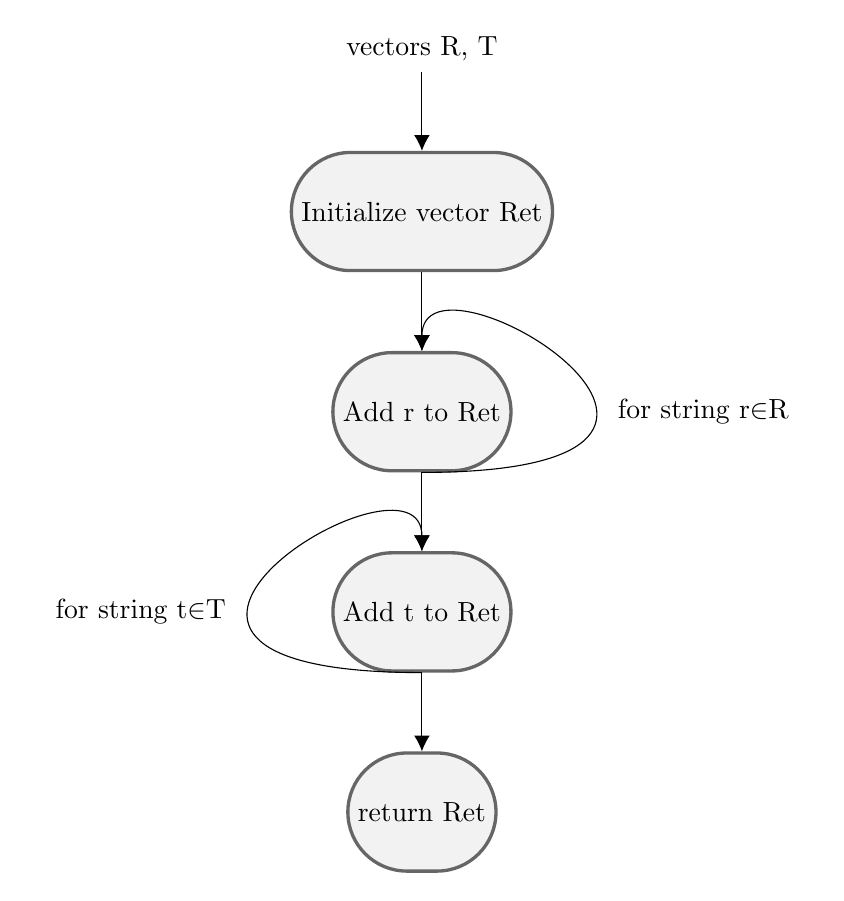
\begin{tikzpicture}[node/.style={rounded rectangle, draw=black!60, fill=black!5, very thick, minimum size=15mm}, bignode/.style={rounded rectangle, draw=black!60, fill=black!5, very thick, minimum size=20mm}, emptynode/.style={draw=none, fill=none, very thick, minimum size=1mm}]
    
    %Nodes
    \node[emptynode](inputs){vectors R, T};
    \node[node](initialize)[below=of inputs]{Initialize vector Ret};
    \node[node](add_r)[below=of initialize]{Add r to Ret};
    \node[node](add_t)[below=of add_r]{Add t to Ret};
    \node[node](return)[below=of add_t]{return Ret};
    \node[emptynode](rtext)[right=1.2cm of add_r]{for string r$\in$R};
    \node[emptynode](ttext)[left=1.2cm of add_t]{for string t$\in$T};
    
    %Lines
    \draw[->] (inputs.south) -- (initialize.north);
    \draw[->] (initialize.south) -- (add_r.north);
    \draw[->] (add_r.south) -- (add_t.north);
    \draw[->] (add_t.south) -- (return.north);
    \draw[->] (add_r.south) .. controls +(right:5 cm) and +(up:1.5 cm) .. (add_r.north);
    \draw[->] (add_t.south) .. controls +(left:5 cm) and +(up:1.5 cm) .. (add_t.north);
    
    \end{tikzpicture}
    }
    \caption{Join Function}
    \label{fig:join graph}
\end{figure}
\end{minipage}
\hfill
\begin{minipage}{0.5\textwidth}
\begin{figure}[H]
    \centering
    \resizebox{8cm}{!}{
    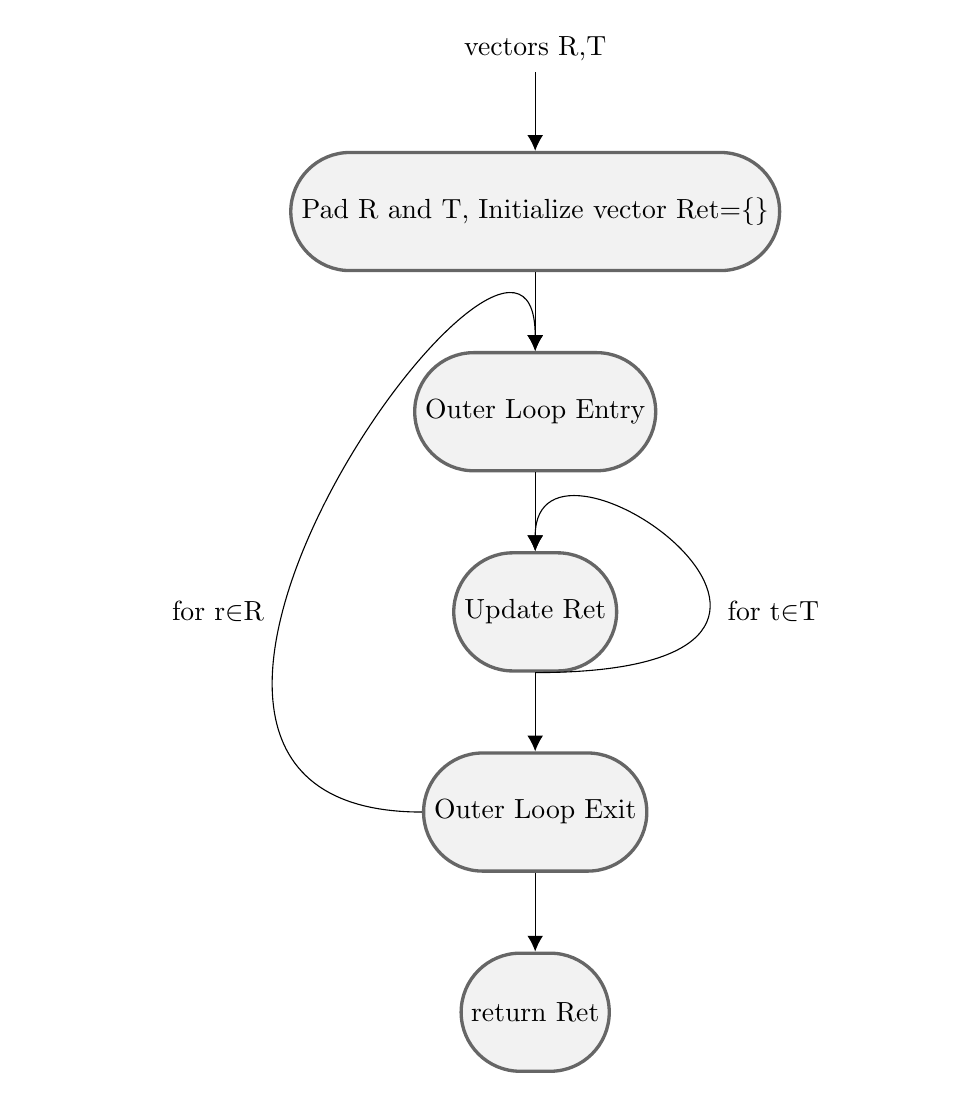
\begin{tikzpicture}[node/.style={rounded rectangle, draw=black!60, fill=black!5, very thick, minimum size=15mm}, bignode/.style={rounded rectangle, draw=black!60, fill=black!5, very thick, minimum size=20mm}, emptynode/.style={draw=none, fill=none, very thick, minimum size=1mm}]
    
    %Nodes
    \node[emptynode](inputs){vectors R,T};
    \node[node](initialize)[below=of inputs]{Pad R and T, Initialize vector Ret=\{\}};
    \node[node](outer_loop)[below=of initialize]{Outer Loop Entry};
    \node[node](inner_loop)[below=of outer_loop]{Update Ret};
    \node[node](outer_exit)[below=of inner_loop]{Outer Loop Exit};
    \node[node](return)[below=of outer_exit]{return Ret};
    \node[emptynode](inner_text)[right=1.25cm of inner_loop]{for t$\in$T};
    \node[emptynode](outer_text)[left=2.25 cm of inner_loop]{for r$\in$R};
    
    %Lines
    \draw[->] (inputs.south) -- (initialize.north);
    \draw[->] (initialize.south) -- (outer_loop.north);
    \draw[->] (outer_loop.south) -- (inner_loop.north);
    \draw[->] (inner_loop.south) -- (outer_exit.north);
    \draw[->] (outer_exit.south) -- (return.north);
    \draw[->] (inner_loop.south) .. controls +(right:5 cm) and +(up:2cm) .. (inner_loop.north);
    \draw[->] (outer_exit.west) .. controls +(left:5 cm) and +(up:3 cm) .. (outer_loop.north);
    
    \end{tikzpicture}
    }
    \caption{Set\_Intersect Function}
    \label{fig:set_intersect graph}
\end{figure}
\end{minipage}

\begin{minipage}{0.4\textwidth}
\begin{figure}[H]
    \centering
    \resizebox{7.25cm}{!}{
    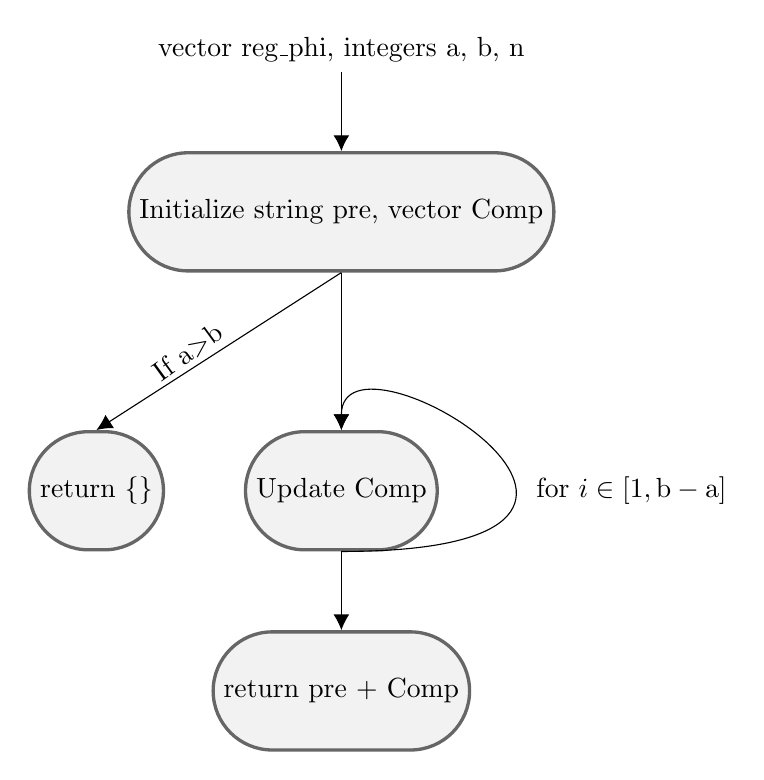
\begin{tikzpicture}[node/.style={rounded rectangle, draw=black!60, fill=black!5, very thick, minimum size=15mm}, bignode/.style={rounded rectangle, draw=black!60, fill=black!5, very thick, minimum size=20mm}, emptynode/.style={draw=none, fill=none, very thick, minimum size=1mm}]
    
    %Nodes
    \node[emptynode](inputs){vector reg\_phi, integers a, b, n};
    \node[node](initialize)[below=of inputs]{Initialize string pre, vector Comp};
    \node[node](loop)[below=2cm of initialize]{Update Comp};
    \node[node](empty)[left=of loop]{return \{\}};
    \node[node](return)[below=of loop]{return pre + Comp};
    \node[emptynode](loop_text)[right=1.1cm of loop]{for $i \in [1, \text{b}-\text{a}]$};
    \node[emptynode](placeholder)[below=0.5cm of initialize]{};
    \node[emptynode](empty_text)[rotate=36, left=1.3cm of placeholder]{If a$>$b};
    
    %Lines
    \draw[->] (inputs.south) -- (initialize.north);
    \draw[->] (initialize.south) -- (empty.north);
    \draw[->] (initialize.south) -- (loop.north);
    \draw[->] (loop.south) -- (return.north);
    \draw[->] (loop.south) .. controls +(right:5 cm) and +(up:1.5 cm) .. (loop.north);
    
    \end{tikzpicture}
    }
    \caption{Reg\_F Function}
    \label{fig:reg_f graph}
\end{figure}
\end{minipage}
\hfill
\begin{minipage}{0.4\textwidth}
\begin{figure}[H]
    \centering
    \resizebox{7.25cm}{!}{
    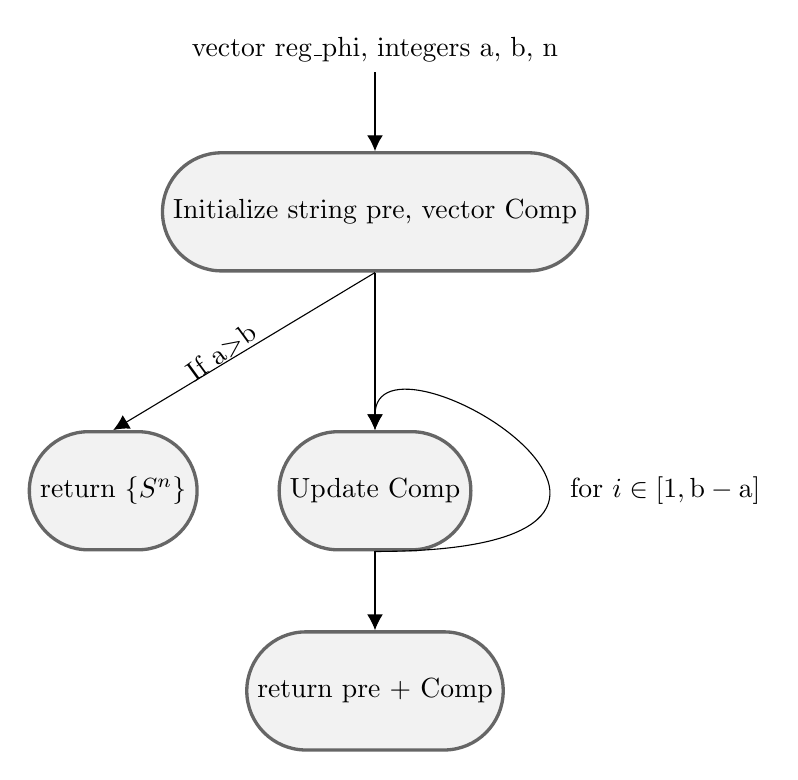
\begin{tikzpicture}[node/.style={rounded rectangle, draw=black!60, fill=black!5, very thick, minimum size=15mm}, bignode/.style={rounded rectangle, draw=black!60, fill=black!5, very thick, minimum size=20mm}, emptynode/.style={draw=none, fill=none, very thick, minimum size=1mm}]
    
    %Nodes
    \node[emptynode](inputs){vector reg\_phi, integers a, b, n};
    \node[node](initialize)[below=of inputs]{Initialize string pre, vector Comp};
    \node[node](loop)[below=2cm of initialize]{Update Comp};
    \node[node](empty)[left=of loop]{return \{$S^n$\}};
    \node[node](return)[below=of loop]{return pre + Comp};
    \node[emptynode](loop_text)[right=1.1cm of loop]{for $i \in [1, \text{b}-\text{a}]$};
    \node[emptynode](placeholder)[below=0.5cm of initialize]{};
    \node[emptynode](empty_text)[rotate=36, left=1.3cm of placeholder]{If a$>$b};
    
    %Lines
    \draw[->] (inputs.south) -- (initialize.north);
    \draw[->] (initialize.south) -- (empty.north);
    \draw[->] (initialize.south) -- (loop.north);
    \draw[->] (loop.south) -- (return.north);
    \draw[->] (loop.south) .. controls +(right:5 cm) and +(up:1.5 cm) .. (loop.north);
    
    \end{tikzpicture}
    }
    \caption{Reg\_G Function}
    \label{fig:reg_g graph}
\end{figure}
\end{minipage}
\vfill
\begin{minipage}{0.4\textwidth}
\begin{figure}[H]
    \centering
    \resizebox{7.25cm}{!}{
    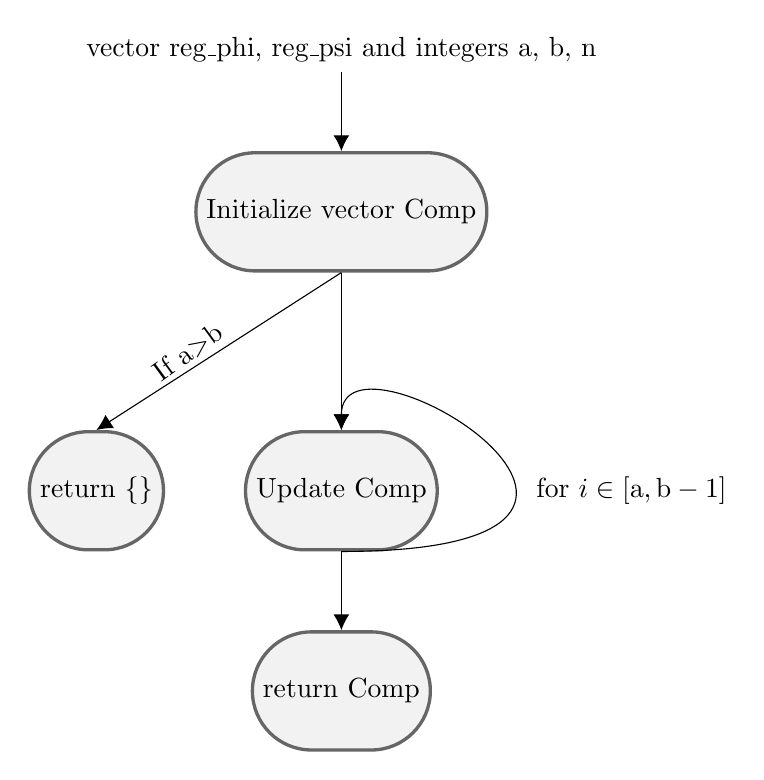
\begin{tikzpicture}[node/.style={rounded rectangle, draw=black!60, fill=black!5, very thick, minimum size=15mm}, bignode/.style={rounded rectangle, draw=black!60, fill=black!5, very thick, minimum size=20mm}, emptynode/.style={draw=none, fill=none, very thick, minimum size=1mm}]
    
    %Nodes
    \node[emptynode](inputs){vector reg\_phi, reg\_psi and integers a, b, n};
    \node[node](initialize)[below=of inputs]{Initialize vector Comp};
    \node[node](loop)[below=2cm of initialize]{Update Comp};
    \node[node](empty)[left=of loop]{return \{\}};
    \node[node](return)[below=of loop]{return Comp};
    \node[emptynode](loop_text)[right=1.1cm of loop]{for $i \in [\text{a}, \text{b}-1]$};
    \node[emptynode](placeholder)[below=0.5cm of initialize]{};
    \node[emptynode](empty_text)[rotate=36, left=1.3cm of placeholder]{If a$>$b};
    
    %Lines
    \draw[->] (inputs.south) -- (initialize.north);
    \draw[->] (initialize.south) -- (empty.north);
    \draw[->] (initialize.south) -- (loop.north);
    \draw[->] (loop.south) -- (return.north);
    \draw[->] (loop.south) .. controls +(right:5 cm) and +(up:1.5 cm) .. (loop.north);
    
    \end{tikzpicture}
    }
    \caption{Reg\_U Function}
    \label{fig:reg_u graph}
\end{figure}
\end{minipage}
\hfill
\begin{minipage}{0.4\textwidth}
\begin{figure}[H]
    \centering
    \resizebox{7.25cm}{!}{
    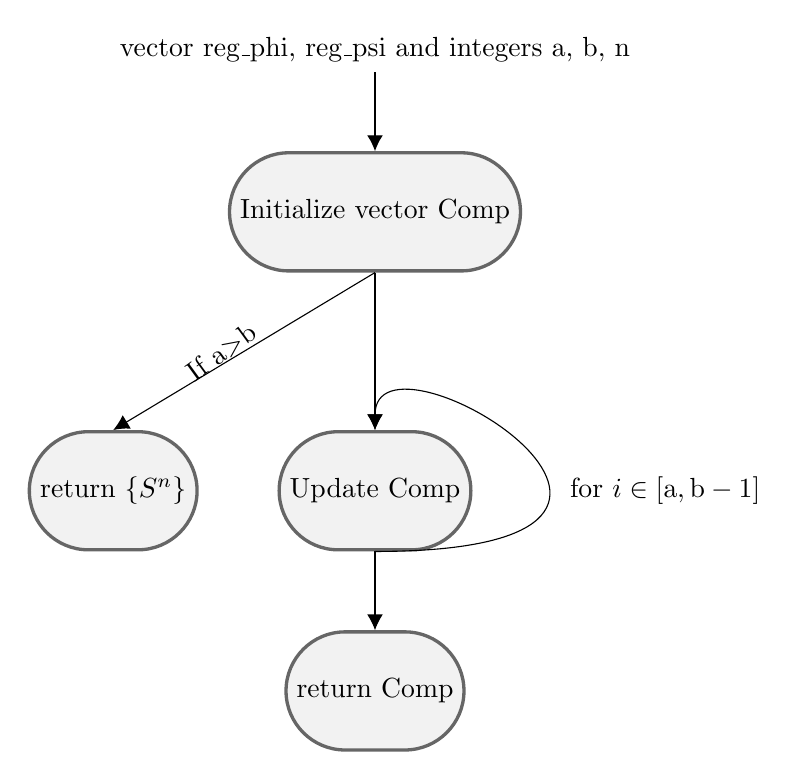
\begin{tikzpicture}[node/.style={rounded rectangle, draw=black!60, fill=black!5, very thick, minimum size=15mm}, bignode/.style={rounded rectangle, draw=black!60, fill=black!5, very thick, minimum size=20mm}, emptynode/.style={draw=none, fill=none, very thick, minimum size=1mm}]
    
    %Nodes
    \node[emptynode](inputs){vector reg\_phi, reg\_psi and integers a, b, n};
    \node[node](initialize)[below=of inputs]{Initialize vector Comp};
    \node[node](loop)[below=2cm of initialize]{Update Comp};
    \node[node](empty)[left=of loop]{return \{$S^n$\}};
    \node[node](return)[below=of loop]{return Comp};
    \node[emptynode](loop_text)[right=1.1cm of loop]{for $i \in [\text{a}, \text{b}-1]$};
    \node[emptynode](placeholder)[below=0.5cm of initialize]{};
    \node[emptynode](empty_text)[rotate=36, left=1.3cm of placeholder]{If a$>$b};
    
    %Lines
    \draw[->] (inputs.south) -- (initialize.north);
    \draw[->] (initialize.south) -- (empty.north);
    \draw[->] (initialize.south) -- (loop.north);
    \draw[->] (loop.south) -- (return.north);
    \draw[->] (loop.south) .. controls +(right:5 cm) and +(up:1.5 cm) .. (loop.north);
    
    \end{tikzpicture}
    }
    \caption{Reg\_R Function}
    \label{fig:reg_r graph}
\end{figure}
\end{minipage}

\begin{landscape}

\begin{figure}[htbp]
    \centering
    \resizebox{20cm}{!}{
    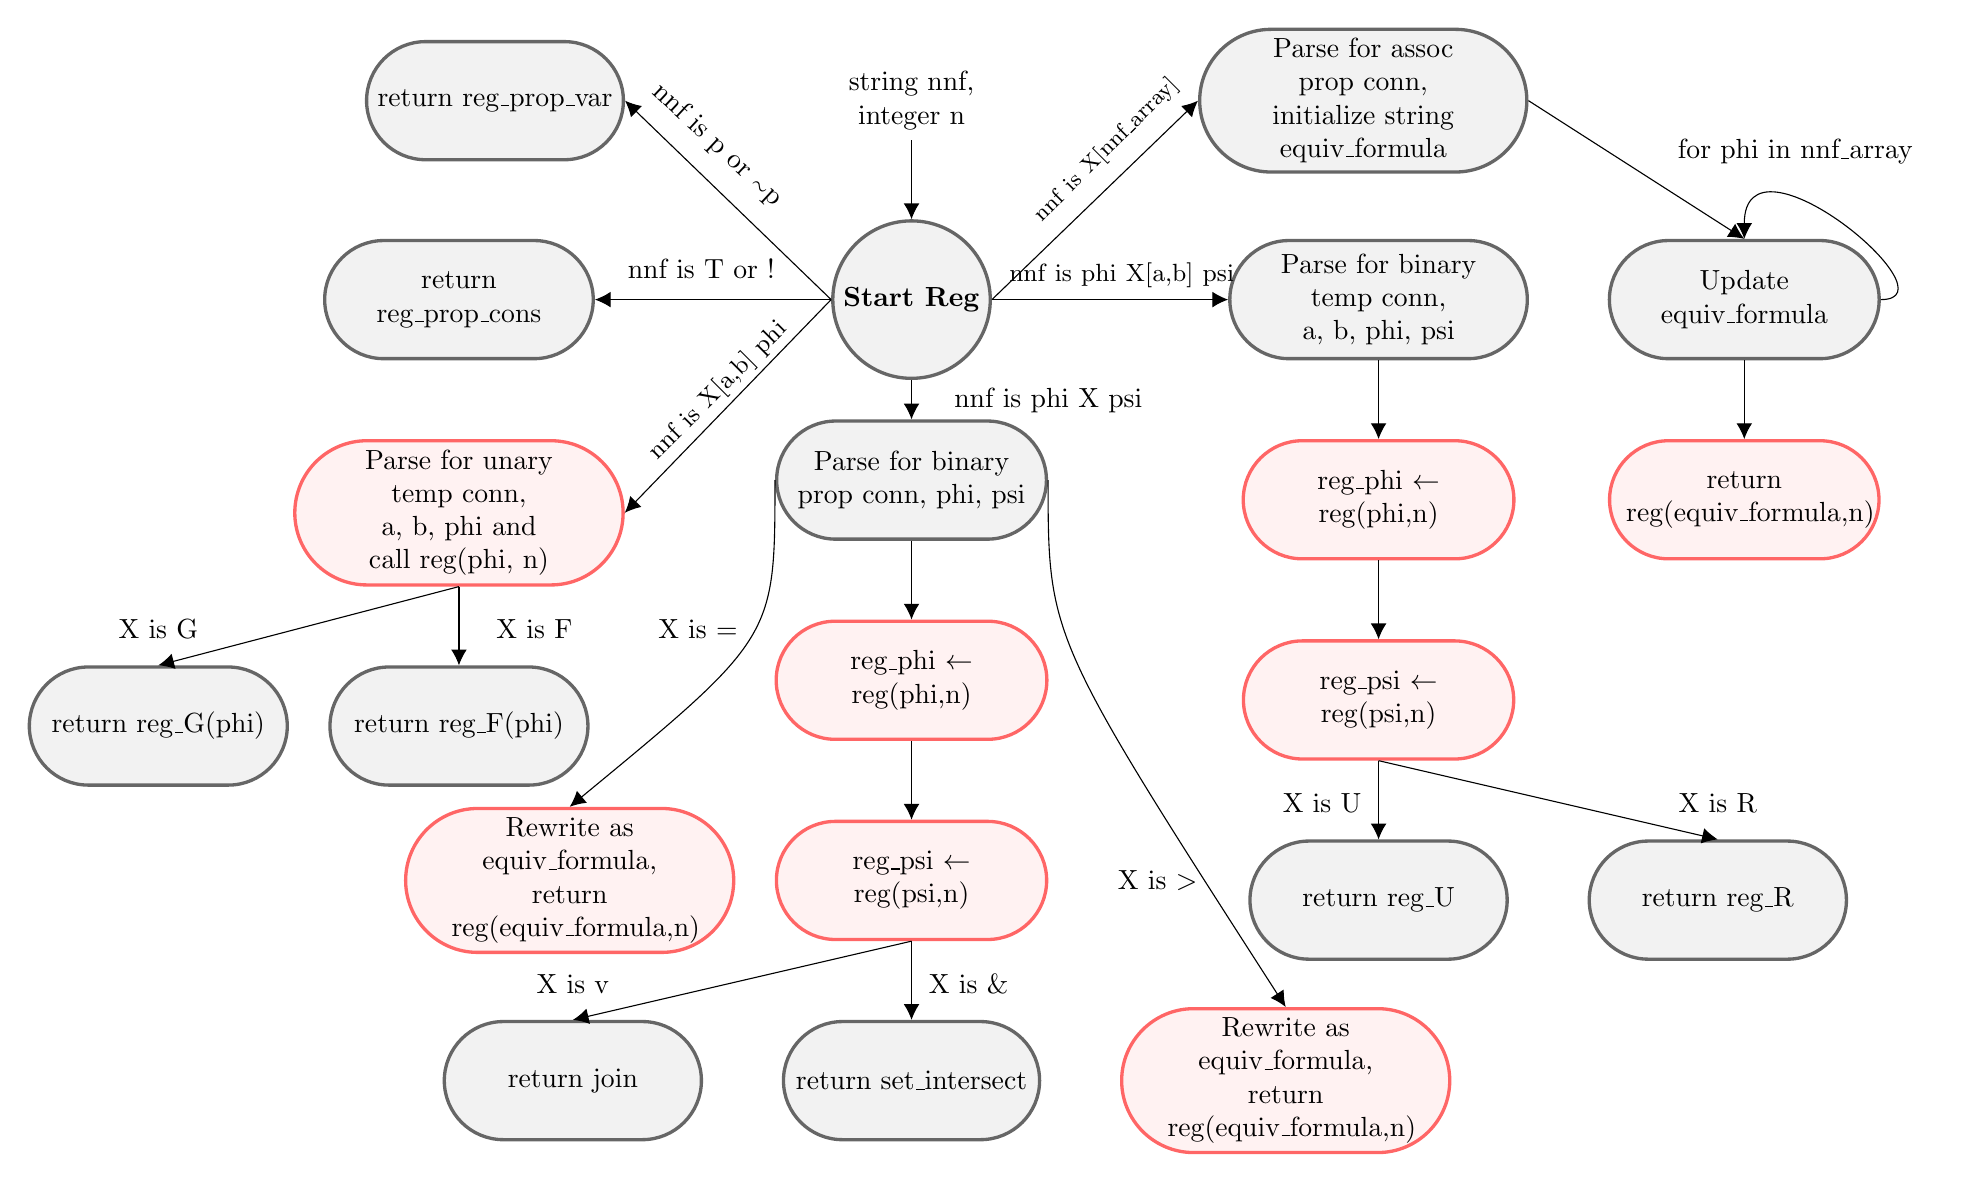
\begin{tikzpicture}[node/.style={rounded rectangle, draw=black!60, fill=black!5, text width=3cm,text centered, very thick, minimum size=15mm}, bignode/.style={rounded rectangle, draw=black!60, fill=black!5, very thick, minimum size=20mm}, emptynode/.style={draw=none, fill=none,text width=3cm,text centered, very thick, minimum size=1mm}, rednode/.style={rounded rectangle, draw=red!60, fill=red!5, text width=3cm,text centered, very thick, minimum size=15mm}]
    
    %Nodes
    \node[emptynode](inputs){string nnf, integer n};
    \node[bignode](start)[below=of inputs]{\textbf{Start Reg}};
    
    \node[node](prop_var)[left=2cm of inputs]{return reg\_prop\_var};
    
    \node[node](prop_cons)[left=3cm of start]{return reg\_prop\_cons};
    
    \node[rednode](parse_unary)[below=1cm of prop_cons]{Parse for unary temp conn, a, b, phi and call reg(phi, n)};
    \node[node](reg_f)[below=1cm of parse_unary]{return reg\_F(phi)};
    \node[node](reg_g)[left=0.5cm of reg_f]{return reg\_G(phi)};
    
    \node[node](parse_binary_prop)[below=0.5cm of start]{Parse for binary prop conn, phi, psi};
    \node[rednode](prop_phi)[below=of parse_binary_prop]{reg\_phi $\leftarrow$ reg(phi,n)};
    \node[rednode](prop_psi)[below=of prop_phi]{reg\_psi $\leftarrow$ reg(psi,n)};
    \node[rednode](equals)[left=0.5cm of prop_psi]{Rewrite as equiv\_formula, return reg(equiv\_formula,n)};
    \node[node](set_intersect)[below=of prop_psi]{return set\_intersect};
    \node[node](join)[left=of set_intersect]{return join};
    \node[rednode](implies)[right=of set_intersect]{Rewrite as equiv\_formula, return reg(equiv\_formula,n)};
    
    \node[node](parse_binary_temp)[right=3cm of start]{Parse for binary temp conn, a, b, phi, psi};
    \node[rednode](temp_phi)[below=of parse_binary_temp]{reg\_phi $\leftarrow$ reg(phi,n)};
    \node[rednode](temp_psi)[below=of temp_phi]{reg\_psi $\leftarrow$ reg(psi,n)};
    \node[node](until)[below=of temp_psi]{return reg\_U};
    \node[node](release)[right=of until]{return reg\_R};
    
    \node[node](parse_assoc)[right=2cm of inputs]{Parse for assoc prop conn, initialize string equiv\_formula};
    \node[node](rewrite_assoc)[right=of parse_binary_temp]{Update equiv\_formula};
    \node[rednode](assoc_return)[below=of rewrite_assoc]{return reg(equiv\_formula,n)};
    
    \node[emptynode](prop_cons_text)[left=0.01cm of start]{nnf is T or !$$~$$};
    \node[emptynode](prop_var_text)[rotate=-43, above=1.1cm of prop_cons_text]{nnf is p or $\scriptstyle{\sim}\textstyle$p};
    
    \node[emptynode](unary_text)[rotate=45, below=0.3cm of prop_cons_text]{\small{nnf is X[a,b] phi}};
    \node[emptynode](reg_g_text)[above=0.2cm of reg_g]{X is G};
    \node[emptynode](reg_f_text)[right=1.5cm of reg_g_text]{X is F};
    
    \node[emptynode](binary_temp_text)[right=0.01cm of start]{\small{nnf is phi X[a,b] psi}$$~$$};
    \node[emptynode](release_text)[above=0.2cm of release]{X is R};
    \node[emptynode](until_text)[left=1.75cm of release_text]{X is U};
    
    \node[emptynode](assoc_text)[rotate=45, above=1.1cm of binary_temp_text]{\footnotesize{nnf is X[nnf\_array]}};
    \node[emptynode](loop_text)[right=1.75cm of parse_assoc]{$$~$$for phi in nnf\_array};
    
    \node[emptynode](binary_prop_text)[right=1.4cm of unary_text]{$$~$$$$~$$$$~$$nnf is phi X psi};
    \node[emptynode](join_text)[above=0.2cm of join]{X is v};
    \node[emptynode](intersect_text)[right=1.75cm of join_text]{X is \&};
    \node[emptynode](implies_text)[right=-0.25cm of prop_psi]{X is $>$};
    \node[emptynode](equals_text)[right=-1.2cm of reg_f_text]{X is =};
    
    %Lines
    \draw[->] (inputs.south) -- (start.north);
    \draw[->] (start.west) -- (prop_var.east);
    \draw[->] (start.west) -- (prop_cons.east);
    \draw[->] (start.west) -- (parse_unary.east);
    \draw[->] (parse_unary.south) -- (reg_g.north);
    \draw[->] (parse_unary.south) -- (reg_f.north);
    \draw[->] (start.south) -- (parse_binary_prop.north);
    \draw[->] (parse_binary_prop.south) -- (prop_phi.north);
    \draw[->] (prop_phi.south) -- (prop_psi.north);
    \draw[->] (prop_psi.south) -- (set_intersect.north);
    \draw[->] (prop_psi.south) -- (join.north);
    \draw[->] (parse_binary_prop.east) .. controls +(down:2cm) .. (implies.north);
    \draw[->] (parse_binary_prop.west) .. controls +(down:2cm) .. (equals.north);
    \draw[->] (start.east) -- (parse_binary_temp.west);
    \draw[->] (parse_binary_temp.south) -- (temp_phi.north);
    \draw[->] (temp_phi.south) -- (temp_psi.north);
    \draw[->] (temp_psi.south) -- (until.north);
    \draw[->] (temp_psi.south) -- (release.north);
    \draw[->] (start.east) -- (parse_assoc.west);
    \draw[->] (parse_assoc.east) -- (rewrite_assoc.north);
    \draw[->] (rewrite_assoc.south) -- (assoc_return.north);
    \draw[->] (rewrite_assoc.east) .. controls +(right:1 cm) and +(up:1.5 cm) .. (rewrite_assoc.north);
    
    \end{tikzpicture}
    }
    $$~$$
    \caption{Control Flow of Reg. Red nodes indicate a recursive call to Reg.}
    \label{fig:big boy}
\end{figure}
\end{landscape}
\end{document}
